% Options for packages loaded elsewhere
\PassOptionsToPackage{unicode}{hyperref}
\PassOptionsToPackage{hyphens}{url}
\PassOptionsToPackage{dvipsnames,svgnames,x11names}{xcolor}
%
\documentclass[
  10pt,
]{krantz}
\usepackage{amsmath,amssymb}
\usepackage{lmodern}
\usepackage{setspace}
\usepackage{iftex}
\ifPDFTeX
  \usepackage[T1]{fontenc}
  \usepackage[utf8]{inputenc}
  \usepackage{textcomp} % provide euro and other symbols
\else % if luatex or xetex
  \usepackage{unicode-math}
  \defaultfontfeatures{Scale=MatchLowercase}
  \defaultfontfeatures[\rmfamily]{Ligatures=TeX,Scale=1}
\fi
% Use upquote if available, for straight quotes in verbatim environments
\IfFileExists{upquote.sty}{\usepackage{upquote}}{}
\IfFileExists{microtype.sty}{% use microtype if available
  \usepackage[]{microtype}
  \UseMicrotypeSet[protrusion]{basicmath} % disable protrusion for tt fonts
}{}
\makeatletter
\@ifundefined{KOMAClassName}{% if non-KOMA class
  \IfFileExists{parskip.sty}{%
    \usepackage{parskip}
  }{% else
    \setlength{\parindent}{0pt}
    \setlength{\parskip}{6pt plus 2pt minus 1pt}}
}{% if KOMA class
  \KOMAoptions{parskip=half}}
\makeatother
\usepackage{xcolor}
\IfFileExists{xurl.sty}{\usepackage{xurl}}{} % add URL line breaks if available
\IfFileExists{bookmark.sty}{\usepackage{bookmark}}{\usepackage{hyperref}}
\hypersetup{
  pdftitle={Arts escèniques},
  pdfauthor={Ramiro Palau Gregori},
  colorlinks=true,
  linkcolor={Maroon},
  filecolor={Maroon},
  citecolor={Blue},
  urlcolor={Blue},
  pdfcreator={LaTeX via pandoc}}
\urlstyle{same} % disable monospaced font for URLs
\usepackage[left=3cm,right=3cm,top=0.85cm,bottom=3cm]{geometry}
\usepackage{color}
\usepackage{fancyvrb}
\newcommand{\VerbBar}{|}
\newcommand{\VERB}{\Verb[commandchars=\\\{\}]}
\DefineVerbatimEnvironment{Highlighting}{Verbatim}{commandchars=\\\{\}}
% Add ',fontsize=\small' for more characters per line
\usepackage{framed}
\definecolor{shadecolor}{RGB}{248,248,248}
\newenvironment{Shaded}{\begin{snugshade}}{\end{snugshade}}
\newcommand{\AlertTok}[1]{\textcolor[rgb]{0.94,0.16,0.16}{#1}}
\newcommand{\AnnotationTok}[1]{\textcolor[rgb]{0.56,0.35,0.01}{\textbf{\textit{#1}}}}
\newcommand{\AttributeTok}[1]{\textcolor[rgb]{0.77,0.63,0.00}{#1}}
\newcommand{\BaseNTok}[1]{\textcolor[rgb]{0.00,0.00,0.81}{#1}}
\newcommand{\BuiltInTok}[1]{#1}
\newcommand{\CharTok}[1]{\textcolor[rgb]{0.31,0.60,0.02}{#1}}
\newcommand{\CommentTok}[1]{\textcolor[rgb]{0.56,0.35,0.01}{\textit{#1}}}
\newcommand{\CommentVarTok}[1]{\textcolor[rgb]{0.56,0.35,0.01}{\textbf{\textit{#1}}}}
\newcommand{\ConstantTok}[1]{\textcolor[rgb]{0.00,0.00,0.00}{#1}}
\newcommand{\ControlFlowTok}[1]{\textcolor[rgb]{0.13,0.29,0.53}{\textbf{#1}}}
\newcommand{\DataTypeTok}[1]{\textcolor[rgb]{0.13,0.29,0.53}{#1}}
\newcommand{\DecValTok}[1]{\textcolor[rgb]{0.00,0.00,0.81}{#1}}
\newcommand{\DocumentationTok}[1]{\textcolor[rgb]{0.56,0.35,0.01}{\textbf{\textit{#1}}}}
\newcommand{\ErrorTok}[1]{\textcolor[rgb]{0.64,0.00,0.00}{\textbf{#1}}}
\newcommand{\ExtensionTok}[1]{#1}
\newcommand{\FloatTok}[1]{\textcolor[rgb]{0.00,0.00,0.81}{#1}}
\newcommand{\FunctionTok}[1]{\textcolor[rgb]{0.00,0.00,0.00}{#1}}
\newcommand{\ImportTok}[1]{#1}
\newcommand{\InformationTok}[1]{\textcolor[rgb]{0.56,0.35,0.01}{\textbf{\textit{#1}}}}
\newcommand{\KeywordTok}[1]{\textcolor[rgb]{0.13,0.29,0.53}{\textbf{#1}}}
\newcommand{\NormalTok}[1]{#1}
\newcommand{\OperatorTok}[1]{\textcolor[rgb]{0.81,0.36,0.00}{\textbf{#1}}}
\newcommand{\OtherTok}[1]{\textcolor[rgb]{0.56,0.35,0.01}{#1}}
\newcommand{\PreprocessorTok}[1]{\textcolor[rgb]{0.56,0.35,0.01}{\textit{#1}}}
\newcommand{\RegionMarkerTok}[1]{#1}
\newcommand{\SpecialCharTok}[1]{\textcolor[rgb]{0.00,0.00,0.00}{#1}}
\newcommand{\SpecialStringTok}[1]{\textcolor[rgb]{0.31,0.60,0.02}{#1}}
\newcommand{\StringTok}[1]{\textcolor[rgb]{0.31,0.60,0.02}{#1}}
\newcommand{\VariableTok}[1]{\textcolor[rgb]{0.00,0.00,0.00}{#1}}
\newcommand{\VerbatimStringTok}[1]{\textcolor[rgb]{0.31,0.60,0.02}{#1}}
\newcommand{\WarningTok}[1]{\textcolor[rgb]{0.56,0.35,0.01}{\textbf{\textit{#1}}}}
\usepackage{longtable,booktabs,array}
\usepackage{calc} % for calculating minipage widths
% Correct order of tables after \paragraph or \subparagraph
\usepackage{etoolbox}
\makeatletter
\patchcmd\longtable{\par}{\if@noskipsec\mbox{}\fi\par}{}{}
\makeatother
% Allow footnotes in longtable head/foot
\IfFileExists{footnotehyper.sty}{\usepackage{footnotehyper}}{\usepackage{footnote}}
\makesavenoteenv{longtable}
\usepackage{graphicx}
\makeatletter
\def\maxwidth{\ifdim\Gin@nat@width>\linewidth\linewidth\else\Gin@nat@width\fi}
\def\maxheight{\ifdim\Gin@nat@height>\textheight\textheight\else\Gin@nat@height\fi}
\makeatother
% Scale images if necessary, so that they will not overflow the page
% margins by default, and it is still possible to overwrite the defaults
% using explicit options in \includegraphics[width, height, ...]{}
\setkeys{Gin}{width=\maxwidth,height=\maxheight,keepaspectratio}
% Set default figure placement to htbp
\makeatletter
\def\fps@figure{htbp}
\makeatother
% Make links footnotes instead of hotlinks:
\DeclareRobustCommand{\href}[2]{#2\footnote{\url{#1}}}
\setlength{\emergencystretch}{3em} % prevent overfull lines
\providecommand{\tightlist}{%
  \setlength{\itemsep}{0pt}\setlength{\parskip}{0pt}}
\setcounter{secnumdepth}{5}
\usepackage{booktabs}
\usepackage[catalan]{babel}
\usepackage{longtable}

%no se  ue fan
%\usepackage[bf,singlelinecheck=off]{caption}
%\usepackage{Alegreya}
%\usepackage[scale=.7]{sourcecodepro}
%\usepackage{framed,color}

\usepackage[skins]{tcolorbox}

\definecolor{colortip}{RGB}{81,183,73}
\definecolor{colornote}{RGB}{119,136,153}
\definecolor{colorwarn}{RGB}{255,83,59}
\definecolor{colorinfo}{RGB}{92, 122, 234}
\definecolor{colorcuidao}{RGB}{251,188,5}

\tcbset{
  colbacktitle=white,
  enhanced,
  boxrule=9pt,
  sharp corners,
  attach boxed title to top left={yshift=-1.5mm, xshift=5mm},
  colback=white, 
  coltext=black, 
  leftrule=.3mm,
  rightrule=.3mm,
  bottomrule=.3mm,
  toprule=.3mm,
  boxsep=1pt, 
  arc=4pt 
}
\newtcolorbox{rmdcuidao}[1]{
  title=#1,
  drop small lifted shadow,
  coltitle=colorcuidao,
  colframe=colorcuidao, 
  colback=colorcuidao!5!
}
\newtcolorbox{rmdtip}[1]{
  title=#1,
  drop small lifted shadow,
  coltitle=colortip,
  colframe=colortip, 
  colback=colortip!5!
}

\newtcolorbox{rmdnote}[1]{
  title=#1,
  drop small lifted shadow,
  coltitle=colornote,
  colframe=colornote,
  colback=colornote!5!
}

\newtcolorbox{rmdwarn}[1]{
  title=#1,
  drop small lifted shadow,
  coltitle=colorwarn,
  colframe=colorwarn,
  colback=colorwarn!5!
}

\newtcolorbox{rmdinfo}{
  drop small lifted shadow,
  coltitle=colorinfo,
  colframe=colorinfo,
  colback=colorinfo!5!,
  %capture=hbox
}

%\makeatother
% marca d'aigua
% https://github.com/callegar/LaTeX-draftwatermark
% https://github.com/callegar/LaTeX-everypage
% https://ctan.org/pkg/draftwatermark
% draftwatermark espacio inestable everypage
%\usepackage[angle=270,text=Espacio\ inestable,color=gray,pos={0.5in,3.5in},scale=0.25]{draftwatermark}
% draftwatermark 和 everypage 由同一个人维护,后者将停止维护
% https://github.com/CTeX-org/ctex-kit/issues/331
%\RecustomVerbatimEnvironment{Highlighting}{Verbatim}{commandchars=\\\{\}}
\ifLuaTeX
  \usepackage{selnolig}  % disable illegal ligatures
\fi
\usepackage[]{natbib}
\bibliographystyle{apalike}

\title{Arts escèniques}
\usepackage{etoolbox}
\makeatletter
\providecommand{\subtitle}[1]{% add subtitle to \maketitle
  \apptocmd{\@title}{\par {\large #1 \par}}{}{}
}
\makeatother
\subtitle{Projecte de pràctiques d'empresa del grau\\
F.P. ASISX\\
I.E. Maria Enriquez\\
\emph{Gandia 2022} Versio web i altres formats en \url{https://incitato.github.io}}
\author{Ramiro Palau Gregori}
\date{2022-06-12}

\begin{document}
\maketitle

{
\hypersetup{linkcolor=}
\setcounter{tocdepth}{2}
\tableofcontents
}
\setstretch{1}
\hypertarget{a-proposit-del-treball}{%
\chapter*{A proposit del treball}\label{a-proposit-del-treball}}


Documentació dels projectes proposats a realitzar en el desenvolupament de les pràctiques realitzades en \textbf{Espacio Inestable}. Aquest manual servira de base per desenvolupar posteriorment un mes detallat per deixar-lo per als propers administradors de la sala..

El llibre encara està en fase de proves, igual que part de la documentació. Mes be, es una recopilació de procediments per implementar serveis, i apunts per resoldre problemes. El projecte està en fase de proves d'aprenentatge dels recursos a implantar, a punt de passar a una verdadera simulació.

Es va fer una primera fase en Virtual Box, per provar els serveis i elegir els que millor s'adaptaven al propòsit del projecte. Una vegada triats, vam buscar un hypervisor de tipus 1, passant a estudiar com fer-los funcionar en el nou entorn. Les alternatives van ser Xen i Proxmox, de codi lliure, elegint finalment Proxmox. La GUI per configurar-lo no ten limitacions com les que vaig trobar per a Xen, la majoria trial 30 dies, o versions incompletes community.

Vam visualitzar en KVM, ja que la base de la host és una ubuntu, i encara que Proxmox està basat en Debian, i existeix un paquet .deb per instal·lar en aquesta distribució, no és compatible en Ubuntu directament.

En la tercera fase, s'instal·lara directament en Debian, i tindrem accés directe a les targetes de xarxa, no fent ponts linux a KVM i d'aci a les VM, i als discs o particions, no havent de fer volums virtuals per simular els verdaders.

\hypertarget{propuxf2sit}{%
\section*{Propòsit}\label{propuxf2sit}}


L'empresa vol desenvolupar els seguents serveis.

\begin{enumerate}
\def\labelenumi{\arabic{enumi}.}
\tightlist
\item
  Implantar un sistema d'accés a internet wifi per al públic que entre en les instal·lacions.
\item
  Implantar un sistema de gravació de les obres que es representen per reproducció en continu o tindre una còpia per després editar-les.
\item
  Un entorn col·laboratiu per als empleats.
\end{enumerate}

Es proposa la següent solució

\begin{enumerate}
\def\labelenumi{\arabic{enumi}.}
\tightlist
\item
  Instala.lacio de dos punts d'accés wifi d'alta capacitat UniFi.
\item
  Una xarxa i sistema cctv de gravació de video amb càmeres IP
\item
  Un entorn de treball col·laboratiu tipus Nextcloud, que inclou serveis de missatgeria, entorn ofimàtic\ldots{}
\item
  Un servidor per allotjar les VM dels serveis i el NAS d'emmagatzemament dels recursos centralitzat.
\item
  Instal·lacio d'una xarxa per donar accés als recursos.
\end{enumerate}

En els propers capitols s'anirà detallant la forma de portar-ho a terme.

\hypertarget{plan-b}{%
\subsection*{Plan B}\label{plan-b}}


En els capitols següents s'estudia la forma d'implementar-ho perquè siga en un futur més fàcilment escalable. El projecte ha d'estar acabat en september, i s'està a l'espera que siguen concedides les subvencions. Si correra presa per posar-lo en funcionament, directament es faria en Truenas, com a base del sistema, ja que té la capacitat de visualitzar, disposa d'alguns dels serveis com Nextcloud com a connector. Instal·lem en un Jail, i ja ho tenim configurat. La política de grups i usuaris, es pot fer des del mateix Truenas, ames del firewall, i OpneVPN. Seria una xarxa molt més simple, inclòs, no fent VPN i directament traure fora, port forwarding, els ports de Nextcloud i Zonemindre. Un RAID 1 per a les dades, per tindre redundància.

Com pensava que tenia temps, craso error, m'he entretingut complicar-me la vida.

\hypertarget{agrauxefments}{%
\section*{Agraïments}\label{agrauxefments}}


Agraïments als tutors:

Pablo Navarro Mon

Jacobo Pallares Burriel

Ulisses Alonso

Pels \href{https://www.levante-emv.com/cultura/2022/06/06/aceleremonos-66978856.html}{ànims}, la paciència i llibertat que m'han deixat per desenvolupar el projecte.

\begin{verbatim}
Sin noticias de Gurb (Eduardo Mendoza)

- ¿qué alternativa le ves?
- Bueno, pues quedarnos en éste.
- ¿Y hacer qué?
- Uf, mogollón de cosas.
- Como por ejemplo qué.
- Montamos un bar tú y yo.
- Mira qué bien:
\end{verbatim}

\hypertarget{infraestructura}{%
\chapter{Infraestructura}\label{infraestructura}}

Definiren la distribució dels espais en el local de l'empresa i la configuració de la xarxa a muntar, per donar els serveis requerits.

\hypertarget{xarxa-per-a-la-sala}{%
\section{Xarxa per a la sala}\label{xarxa-per-a-la-sala}}

Es proposa la següent configuració de xarxa per a la sala.

\begin{itemize}
\tightlist
\item
  Xarxa de Video per al \emph{registrament / reproducció en línia} de les obres de teatre.
\item
  Xarxa de wifi, pública i privada.
\item
  Xarxa Privada per als treballadors, amb connexió externa per VPN.
\item
  Xarxa d'administració
\end{itemize}

\hypertarget{descripciuxf3-de-les-installacions}{%
\section{Descripció de les instal·lacions}\label{descripciuxf3-de-les-installacions}}

Pla de la sala

\begin{figure}
\centering
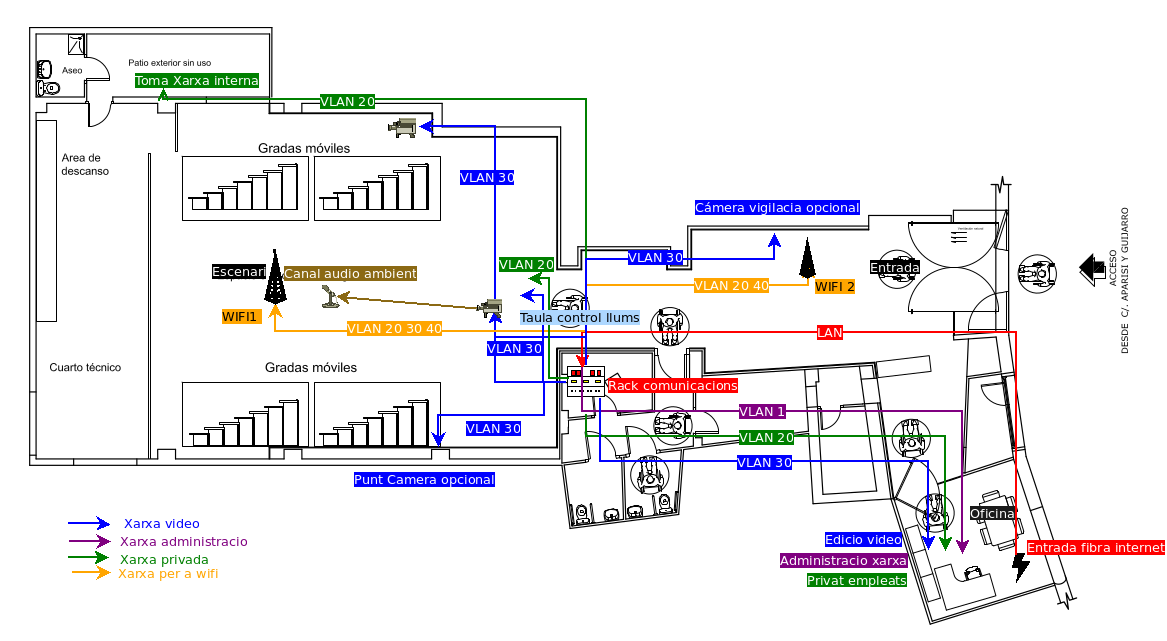
\includegraphics{imatges/teatre.png}
\caption{Pla de la sala}
\end{figure}

La sala la podem dividir en 4 espais

\begin{itemize}
\tightlist
\item
  Oficina
\item
  Escenari
\item
  Entrada
\item
  Rebosts, en un d'ells posarem el Rack de comunicació i servidor.
\end{itemize}

\hypertarget{oficina}{%
\subsection{Oficina}\label{oficina}}

En l'oficina tenim l'entrada de la connexió de fibra a internet. Des d'aci portem la connexió de xarxa al rack de comunicacions on tenim la infraestructura de la xarxa, el commutador i el servidor.

Des del rack de comunicacions, tornarem connexions de xarxa cap a l'oficina per donar accés als serveis interns VLAN 20, per poder fer l'edició de video i la reproducció en línia si es donara el cas VLAN 30, i una toma de xarxa per realitzar l'administració VLAN 1.

Per facilitar el seu ús, cadascuna d'aquestes per cables separats acabant en una roseta etiquetada segons VLAN.

\hypertarget{sala-despera}{%
\subsection{Sala d'espera}\label{sala-despera}}

En aquest espai, tenim l'ordinador de venda d'entrades al que li donarem connexió, siga directa al commutador, per la connexió de l'oficina o el canal wifi privant.

En el centre de la sala aniria l'antena wifi 2 tipus PoE connectada al nucli de comunicacions per on tindrem VLAN 20 30 separades en dos SSID Privat i Pública.

També posarem una connexió VLAN 30 per si en un futur, es vol reciclar alguna camera per fer de videovigilància. Font a aquesta connexió hi ha un projector al qual li podem posar una roseta amb la VLAN 20 per reproduir arxius de video editats o presentacions des de VLAN 20 (no està dibuixada per claredat de l'esquema).

\hypertarget{escenari}{%
\subsection{Escenari}\label{escenari}}

\begin{itemize}
\item
  En la sala d'espectacles es traurien 4 connexions de la xarxa video \emph{VLAN 30}.

  \begin{itemize}
  \tightlist
  \item
    \textbf{Central}, baix de la taula de llums, on es connectara un Camera ip PoE fixa.
  \item
    \textbf{Lateral}, una a cada banda de l'escenari, camera desmuntable que es pot traslladar lateralment segons les necessitats de l'obra representada. Es recomana que aquesta siga del tipus PTZ. Podent ser col·locada a la dreta o l'esquerra de l'escenari.
  \item
    Una toma en la taula de llums, per poder retransmetre el video en la mateixa representació.
  \item
    Una connexió per l'antena wifi, per poder ser sevir el movil com a camera web, amb app tipus \href{https://play.google.com/store/apps/details?id=com.pas.webcam\&gl=US}{IP webcam}, \href{https://iriun.com/}{Irun webcam}.
  \item
    \textbf{Micròfon ambient} que el connectarem a la camera central que es fixa.
  \end{itemize}
\item
  Una connexió per a la xarxa pública \emph{VLAN 40}, per l'antena wifi, al centre del sostre de l'escenari, per donar millor cobertura.
\item
  Un punt de connexió en el vestuari a la VLAN 20, per comunicació amb la xarxa interna, que pot donar cobertura per cable a l'escenari en cas de conferències, o altres actes que necessiten bona connexió de xarxa.
\item
  Un altre punt de connexió a aquesta VLAN 20 en la taula de llums, per tindre accés als recursos interns i poder fer comunicació pel TALK de Nextcloud amb els vestuaris i oficines.
\end{itemize}

\hypertarget{rebost}{%
\subsection{Rebost}\label{rebost}}

En un dels rebosts que hi ha en la sala, muntarem el Rack de comunicacions, aprofitarem en el que està instal·lada la infraestructura de luminació del escenari, que disposa de bones connexions elèctriques, bon aïllat acustica i tèrmicament.

\hypertarget{descripciuxf3-de-les-xarxes}{%
\section{Descripció de les xarxes}\label{descripciuxf3-de-les-xarxes}}

\emph{La configuració de les xarxes, la farem amb 4 VLAN.}

\hypertarget{vlan-1-administraciuxf3}{%
\subsection{VLAN 1 Administració}\label{vlan-1-administraciuxf3}}

És la xarxa per on s'executaran les tasques d'administració dels serveis amb ssh, i per on passara tot el tràfic intern entre les diferents VM, autenticació LDAP, recursos d'espai de les aplicacions.

Aquesta xarxa, interna del servidor per open v Switch, i soles tindrà una eixida física a lo'oficina. I una OpenVPN pròpia per gestionar des de l'exterior, amb accés soles per a l'administrador.

\hypertarget{vlan-20-privat}{%
\subsection{VLAN 20 Privat}\label{vlan-20-privat}}

Xarxa amb connexió a internet i als serveis oferits per la sala.

Es donaran els següents accessos.

\begin{enumerate}
\def\labelenumi{\arabic{enumi}.}
\item
  \emph{Taula de llums}, perquè puguen accedir a recursos guardats en el servidor, mantenir comunicació amb el vestuari.
\item
  \emph{Vestuaris}, comunicació o recursos de xarxa a l'escenari.
\item
  \emph{Oficines}, donar accés a recursos del servidor, donar xarxa a telèfon ip instal·lat.
\item
  \emph{Punts wifi}, crearem una segona xarxa amb enquesta Vlan en les antenes wifi de sol accés per als treballadors de la sala.
\end{enumerate}

\hypertarget{vlan-30-video}{%
\subsection{VLAN 30 Video}\label{vlan-30-video}}

Xarxa per la qual anirà el circuit intern de televisió, siga per la reproducció en línia o per fer gravació de les obres en el servidor. No disposara de connexió a internet.

Configurarem accés a aquesta Vlan des del punt wifi de l'escenari, per poder gastar el movil com a camera en les representacions.

\begin{rmdcuidao}{cap connexió a internet}
En la taula de llums, si volen fer servir aquest servei, no volen tindre cap connexió a internet en l'ordinador que gestionen les llums i el video, per no tindre sorpreses de notificacions, correus \ldots{} En meitat d'una representació.

\end{rmdcuidao}

Per poder guardar el tràfic de video d'aquesta xarxa, tenim diverses opcions

\begin{enumerate}
\def\labelenumi{\arabic{enumi}.}
\tightlist
\item
  Muntar en el servidor una LXC de \href{https://zoneminder.com/}{Zonaminder}, \href{https://shinobi.video/}{Shinobi}\ldots{} on gestionar les gravacions de video de les càmeres. Amb aquest tipus de programes NVR es facilita molt la gestió aquesta xarxa.
\end{enumerate}

\begin{rmdinfo}{}
La gravadora (NVR) En un sistema de càmeres de seguretat IP, el NVR (Network Video Recorder) és central que gestiona i emmagatzema les imatges de vídeo. Totes les càmeres IP enviaran les seues dades a les gravadores des de les quals podeu visualitzar en directe o fer còpies de seguretat de les gravacions.

\end{rmdinfo}

\begin{enumerate}
\def\labelenumi{\arabic{enumi}.}
\setcounter{enumi}{1}
\item
  Les càmeres IP es poden gestionar des del seu propi servidor web, on podem configurar l'espai d'emmagatzemament per FTP, SMB \ldots{} Depenent del protocol que utilitzen, es pot compartir l'espai de video de Truenas amb el mateix protocol i programar-ho des de qualsevol connexió VLAN 30.
\item
  Des de l'oficina utilitzant programes tipus OSB per fer la reproducció en línia o copia a l'espai de Truenas
\end{enumerate}

\begin{rmdcuidao}{afegir el servei Truenas}
Haguérem d'afegir el servei Truenas a aquesta xarxa VLAN 30 en el cas 2, i a la VLAN 20 en el cas 3, que en principi no està previst, es planteja fer tot el tràfic de dades per la VLAN 1.

\end{rmdcuidao}

\hypertarget{vlan-40-puxfablica}{%
\subsection{VLAN 40 pública}\label{vlan-40-puxfablica}}

Xarxa amb connexió a internet per al públic general a través dels punts wifi, i totalment aïllada de les altres VLAN.

La podem configurar amb un portal captiu, amb pfSense, amb permís de connectar a certes hores coincidint en les representacions, canviant el password en cada obra, que oferirem al públic per un codi QR. Posar un sistema de tiquets que per a les connexions \ldots{}

Es pot aprofitar aquesta connexió per a redirigir als espectadors en un primer moment a un servidor web propi on publicitar ressenyes de properes obres, donar més informació de l'obra que van a veure, o interactuant amb ells via web en el transcurs de la representació.

\hypertarget{xarxa-interna-dels-serveis}{%
\subsection{Xarxa interna dels serveis}\label{xarxa-interna-dels-serveis}}

El disseny per a la xarxa de cada VM el representem en el següent diagrama, seria afegir les targetes necessaries per a cada VM i connectar-les a les VLAN que necessitem.

\begin{figure}
\centering
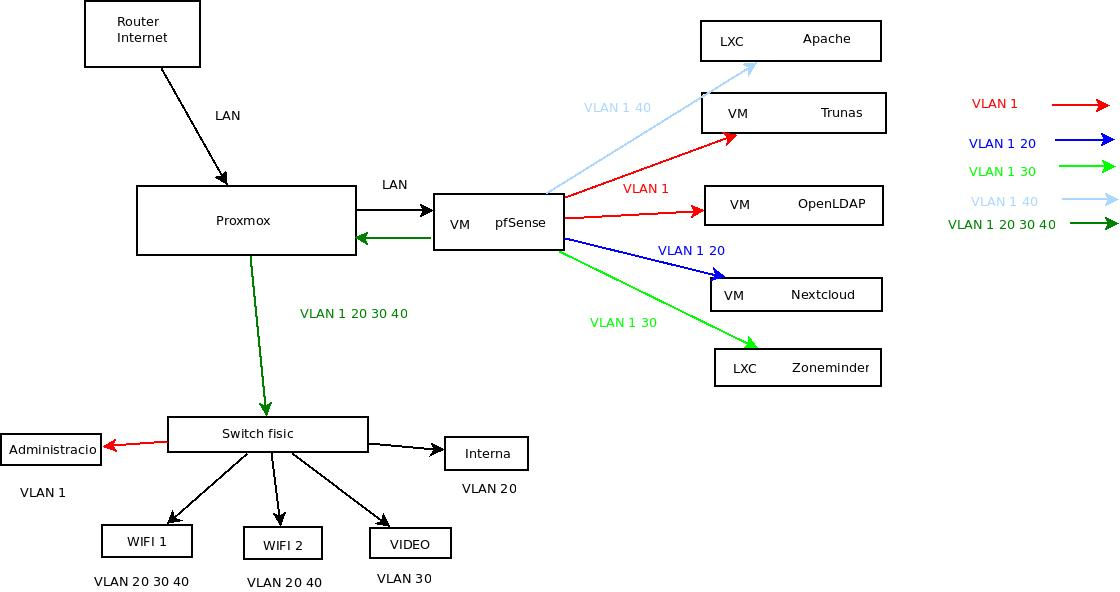
\includegraphics{imatges/proxmox/Xarxa_VLAN.jpeg}
\caption{Esquema de les xarxes}
\end{figure}

Tots els serveis administratius: Compartició d'espai d'emmagatzemament, autenticació LDAP, còpies de seguretat i administració dels serveis, aniran per la VLAN 1. Tots les VM tindran una connexió en aquesta VLAN.

Els serveis per al personal de l'empresa i convidats: Nextcloud i Zoneminder correran per la VLAN 20 que tindrà eixida a l'exterior per les antenes wifi i VPN. Aquesta xarxa sols oferira serveis per HTTPS 443, en un futur es podria plantejar oferir més serveis com correu, SMB, FTP. Pero amb l'entorn Nextcloud, els podem centralitzar amb aquesta aplicació.

La xarxa de video VLAN 30, principalment correra per cable, no disposa de connexió a internet. L'entrada per la xarxa wifi, sols es farà servir per connectar mòbils per fer de web cam en els espectacles, no sent tan fiable aquest tipus de connexió per a la retransmissió de video d'alta qualitat. En els punts de connexió d'aquesta VLAN , taula de llums i oficina, es podrà connectar directament a les càmeres, per poder editar les imatges per altres programes tipus OBS per fer streaming, o retransmetre al mateix espectacle.en directe.

Per acabar, la VLAN 40 estarà aïllada de la resta de xarxes pel firewall de pfSense, Soles sera servida pels punts wifi, La forma de gestionar aquests punts d'accés queda oberta a l'elecció del'empresa. Un password que es proporcionara per codi QR, un sistema de portal captiu, sistema de tiquets\ldots{} La millor opció seria el portal captiu i reencaminar després a un servidor web intern per aquesta xarxa amb promocions de les obres. Aquest servidor web s'implementaria amb un contenidor, ja siga Wordpress, apache amb Pico de fulles estàtiques, en la carpeta conectada, on deixem els fitxers en md per generar les pàgines, estarà compartit amb nextcloud recurs extern, per poder generar-les des d'alli.

\hypertarget{proposta-de-projecte}{%
\chapter{Proposta de projecte}\label{proposta-de-projecte}}

Requeriments de l'empresa

\begin{enumerate}
\def\labelenumi{\arabic{enumi}.}
\tightlist
\item
  Implantar un sistema d'accés a internet wifi per al públic que entre en les instal·lacions.
\item
  Implantar un sistema de gravació de les obres que es representen per reproducció en continu o tindre una còpia per després editar-les.
\item
  Un entorn col·laboratiu per als empleats.
\end{enumerate}

\hypertarget{serveis-proposats}{%
\section{Serveis proposats}\label{serveis-proposats}}

\begin{itemize}
\tightlist
\item
  Entorn de serveis d'allotjament de fitxers Nextcloud, és funcionalment similar a Dropbox, Office 365 o Google Drive quan s'utilitza amb les seues solucions d'oficina integrades Collabora Online o OnlyOffice.
\item
  Servei de comunicació entre membres, per Nextcloud Talk, video, audio o xat.
\item
  Servei de wifi per a la sala, separant tres xarxes.

  \begin{itemize}
  \tightlist
  \item
    Interna, membres de l'equip (internet i xarxa local de serveis) VLAN 20
  \item
    Públic (sols accessos a internet) VLAN 40
  \item
    video (sense accés a internet) VLAN 30
  \end{itemize}
\item
  serveis de video, tipus videovigilància, que ens permet gravar les obres, retransmetre a usuaris autenticats en directe (per veure assajos), veure còpies d'esdeveniments gravats. La forma més senzilla és fent servir solucions NVR tipus Zoneminder o shinobi.
\item
  Aprofitant la wifi pública, habilitar un servidor web intern en aquesta xarxa per promocions, documentació extra de les obres, o interactuar amb el públic.
\end{itemize}

Per portar-lo a terme es requeriria

\begin{enumerate}
\def\labelenumi{\arabic{enumi}.}
\tightlist
\item
  Muntar punts wifi d'alta capacitat.
\item
  Un servidor per allotjar les VM dels serveis, espai per guardar els documents i les gravacions de video.
\item
  Instal·lacio d'una xarxa informàtica, commutador, cablejat, Rack.
\end{enumerate}

\hypertarget{pressupost-del-maquinari}{%
\section{Pressupost del maquinari}\label{pressupost-del-maquinari}}

Es proposa el següent maquinari

\begin{enumerate}
\def\labelenumi{\arabic{enumi}.}
\item
  \href{https://www.ebay.es/itm/125269454776?hash=item1d2aa42fb8:g:aTIAAOSw3ExiXvm5}{Servidor}

  \textbf{Cost 250 euros + iva -\textgreater{} 300 euros}

  \begin{figure}
  \centering
  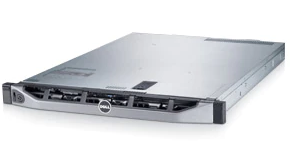
\includegraphics{imatges/serverR320.png}
  \caption{server}
  \end{figure}

  No porta Discs durs.\{width=25\%\}
\item
  Discs durs per al servidor, minim 3 per fer un sistema de seguretat a fallades, i un SSD per al sistema base i les VM. Disposa d'espai per a 4 de connexió en calent dins la seua caixa, si fera falta més, en un futur es posaran, pero ja fora del xassís.

  \textbf{Cost de 4TB, al voltant de 90 euros cada un}

  Referències orientatives \href{https://www.pcbox.com/st4000dm004-seagate-barracuda--st4000dm004-4000gb-3-5--serial-ata-iii/p}{SEAGATE Barracuda ST4000DM004 4000GB 3.5 Serial ATA III} \href{https://www.amazon.es/Seagate-Barracuda-Disco-Interno-cach\%C3\%A9/dp/B0713R3Y6F/ref=sr_1_5?__mk_es_ES=\%C3\%85M\%C3\%85\%C5\%BD\%C3\%95\%C3\%91\&crid=JR7AGWGKGDES\&keywords=hd\%2Bsata\%2B4tb\&qid=1651315567\&sprefix=hd\%2Bsata\%2B4tb\%2Caps\%2C93\&sr=8-5\&th=1}{amazon Barracuda 4TB}
\item
  Switch, \href{https://www.pccomponentes.com/buscar/?query=switch\%2024\%20poe\&or-relevance}{referencies orientatives}
\end{enumerate}

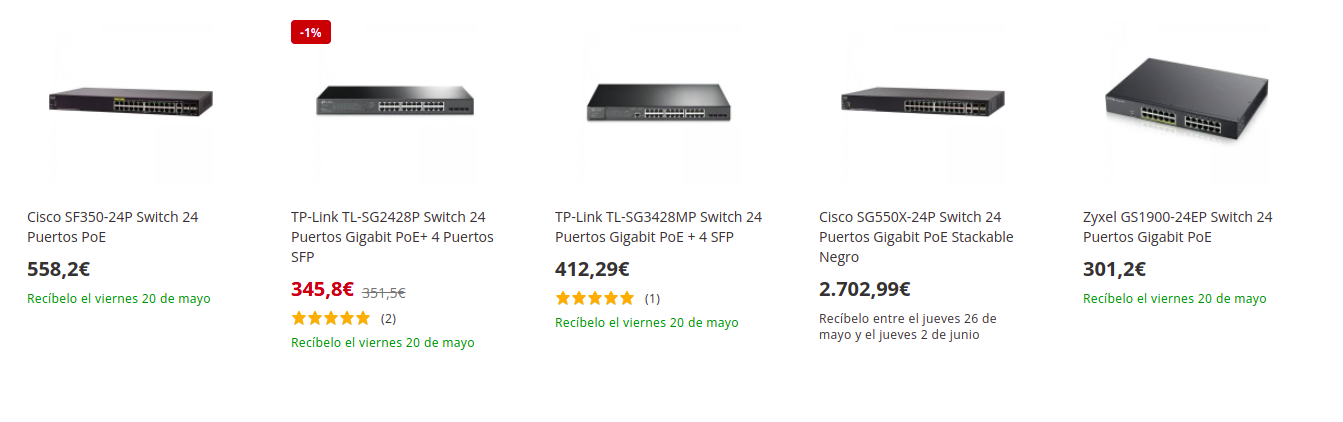
\includegraphics[width=0.8\textwidth,height=\textheight]{imatges/switch.png} Es requereix que siga PoE+ (alimentació elèctrica del dispositiu pel cable LAN) per a les càmeres IP i les dues antenes wifi. De 24 ports. El model s'elegira segons presupost final. \textbf{cost entre 300 i 600}

\begin{enumerate}
\def\labelenumi{\arabic{enumi}.}
\item
  Armari \href{https://www.pccomponentes.com/microconnect-armario-rack-19-6u-600x600mm-negro}{Rack} per al servidor i el switch.\\
  \textbf{Cost Microconnect Armario Rack 19'' 6U 600X600mm Negro 130,56€}
\item
  \href{https://www.pccomponentes.com/buscar/?query=patch\%20panel\&or-relevance}{Patch panel}\\
  \textbf{Cost depen dels ports del switch, al voltant de 30 euros}
\item
  Cablejat i rosetes, Eas contractara una empresa externa especialitzada.
\item
  Antena \href{https://ui.com/wi-fi\#compare}{wifi Unifi}

  \begin{itemize}
  \tightlist
  \item
    U6 Professional \$ 149.00
  \item
    U6 Lite \$ 99.00
  \end{itemize}
\item
  Càmeres ip.
\end{enumerate}

En la sala coneixen una persona que treballa en el món d'imatge i so, esperant recomanacions.

\begin{itemize}
\item
  \textbf{Professional} Sony, pero de 2500 euros no baixen.
\item
  Barates

  \textbf{càmeres amb nightcolor}

  \href{https://www.amazon.es/Exteriores-Seguridad-vigilancia-detecci\%C3\%B3n-humanoide/dp/B09CMRTXCH/ref=sr_1_5?__mk_es_ES=\%C3\%85M\%C3\%85\%C5\%BD\%C3\%95\%C3\%91\&crid=1HGWT0B8AQ04L\&keywords=ptz+Visi\%C3\%B3n+Nocturna+a+Color+poe\&qid=1652043379\&s=tools\&sprefix=ptz+visi\%C3\%B3n+nocturna+a+color+poe\%2Cdiy\%2C95\&sr=1-5}{barata} 67.99 euros

  \href{https://www.amazon.es/Reolink-Seguridad-Seguimiento-Autom\%C3\%A1tico-Outdoor-V3/dp/B099F2LGSB/ref=sr_1_9?__mk_es_ES=\%C3\%85M\%C3\%85\%C5\%BD\%C3\%95\%C3\%91\&crid=1HGWT0B8AQ04L\&keywords=ptz+Visi\%C3\%B3n+Nocturna+a+Color+poe\&qid=1652043379\&s=tools\&sprefix=ptz+visi\%C3\%B3n+nocturna+a+color+poe\%2Cdiy\%2C95\&sr=1-9}{Reolink 5MP PTZ Cámara} 139,99€

  \href{https://www.amazon.es/Reolink-Vigilancia-Bidireccional-Impermeable-RLC-812A/dp/B096K1P2RK/ref=sr_1_10?__mk_es_ES=\%C3\%85M\%C3\%85\%C5\%BD\%C3\%95\%C3\%91\&crid=1HGWT0B8AQ04L\&keywords=ptz+Visi\%C3\%B3n+Nocturna+a+Color+poe\&qid=1652043379\&s=tools\&sprefix=ptz+visi\%C3\%B3n+nocturna+a+color+poe\%2Cdiy\%2C95\&sr=1-10}{fixa reolink 4K} 94,99€
\end{itemize}

\begin{rmdinfo}{Segons fabricant}
Segons fabricant La tecnologia d'avantguarda NightColor us permet obtenir una imatge nítida fins i tot quan és fosc. Aquesta càmera té 2 LED blancs que transmeten els seus raigs infrarojos en una freqüència imperceptible a l'ull humà. Les llums blanques emeten brillants que ofereixen una increïble gamma de NightColor de 66 peus. Amb aquesta potent funció, podeu aconseguir una consciència total sobre allò que no s'havia vist anteriorment i fer-ho d'una manera indetectable.

Pero no se jo. Es pot provar en una a veure com va, si no dona bon resultat es pot posar de camera de vigilància de l'entrada de la sala.

\end{rmdinfo}

\begin{itemize}
\item
  Un poc millor \href{https://www.amazon.es/Amcrest-NightVision-resistente-intemperie-IP8M-2496EW-28MM/dp/B08SMPGF2L/ref=sr_1_1_sspa?__mk_es_ES=\%C3\%85M\%C3\%85\%C5\%BD\%C3\%95\%C3\%91\&crid=B563YL5W8NZG\&keywords=Amcrest\&qid=1652041726\&sprefix=amcrest\%2Caps\%2C93\&sr=8-1-spons\&psc=1\&spLa=ZW5jcnlwdGVkUXVhbGlmaWVyPUEzNU04RVpYSEg2MTNDJmVuY3J5cHRlZElkPUEwODgxOTQwRDUzMkNEVUg0QUVIJmVuY3J5cHRlZEFkSWQ9QTEwMTQxOTBBNzRSODlYRllZNk4md2lkZ2V0TmFtZT1zcF9hdGYmYWN0aW9uPWNsaWNrUmVkaXJlY3QmZG9Ob3RMb2dDbGljaz10cnVl}{Amcrest UltraHD 4K (8 MP) POE IP, càmera exterior, 3840 x 2160, 131 pies NightVision} 129,99€ \href{https://amcrest.com/downloadable/download/attachment/id/22371/}{especificacions}
\item
  Gamma Mitjana \href{https://www.amazon.es/Zowietek-PTZ-Pro-transmisi\%F3n-videoconferencia/dp/B086X637W2/ref=sr_1_2_sspa?keywords=Zowietek\%2BPro\%2BCamera\%2B20X\%2BLive\&qid=1652728314\&sr=8-2-spons\&th=1}{Zowietek PTZ Pro Cámara PTZ} \textbf{Al voltant de 700 euros}
\end{itemize}

D'aquesta gamma hi ha moltes.

\hypertarget{servidor}{%
\chapter{Servidor}\label{servidor}}

\begin{enumerate}
\def\labelenumi{\arabic{enumi}.}
\tightlist
\item
  \href{https://www1.la.dell.com/content/products/productdetails.aspx/poweredge-r320?c=ve\&l=es\&s=corp\&cs=vecorp1}{Servidor}. En \href{https://www.ebay.es/itm/125269454776?hash=item1d2aa42fb8:g:aTIAAOSw3ExiXvm5}{ebai} el podem trobar per uns 250 euros + IVA, amb 64G de ram.
\end{enumerate}

\begin{figure}
\centering
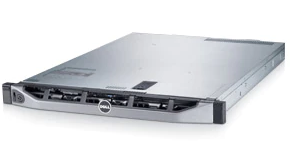
\includegraphics[width=0.3\textwidth,height=\textheight]{imatges/serverR320.png}
\caption{serverR320}
\end{figure}

\textbf{Especificacions}

\begin{figure}
\centering
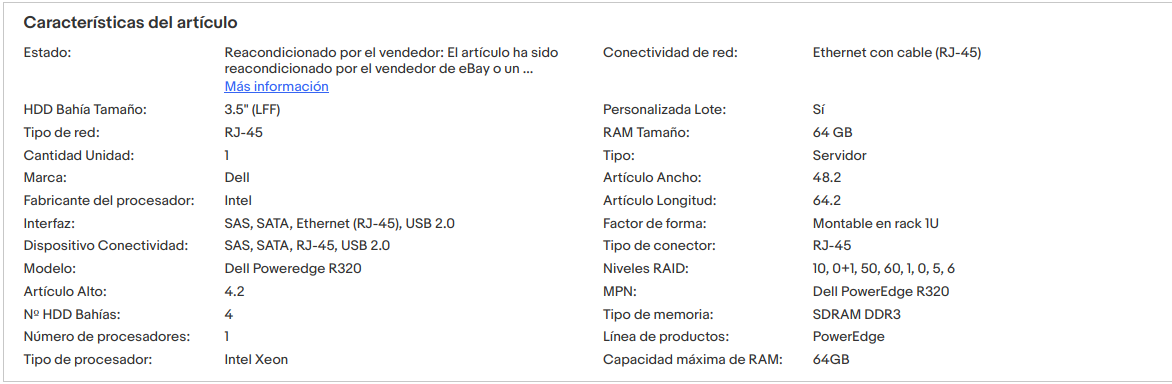
\includegraphics[width=0.8\textwidth,height=\textheight]{imatges/server_hp.png}
\caption{server}
\end{figure}

\begin{rmdnote}{}
\href{https://i.dell.com/sites/csdocuments/Shared-Content_data-Sheets_Documents/ja/jp/Dell-PowerEdge-R320Technical-Guide.pdf}{Documentació del model}, i \href{https://www.dell.com/support/home/en-us/product-support/product/poweredge-r320/docs}{manuals}, \href{https://dl.dell.com/topicspdf/poweredge-r320_owners-manual_en-us.pdf}{owner manual} Compatibilitat amb \href{https://ubuntu.com/certified?category=Server\&vendor=Dell+EMC\&offset=20}{ubuntu server}, és compatible amb la versió 14 i posteriors. En la fulla de \href{https://www.dell.com/support/contents/en-us/article/Product-Support/Self-support-Knowledgebase/enterprise-resource-center/server-operating-system-support}{Dell}

\end{rmdnote}

\begin{rmdinfo}{}
És compatible amb la \href{https://linux.dell.com/files/supportmatrix/Ubuntu_Support_Matrix.pdf}{versió 14.04 LTS}, no apareix en la llista, manté la compatibilitat hardware amb les més recents. És un servidor del 2014, pero per als requisits que requerim, pocs usuaris, tràfic limitat, és suficient. A una mala Posem \href{https://www.centos.org/}{CentOS}

\end{rmdinfo}

\emph{Dimensions servidor}

\begin{figure}
\centering
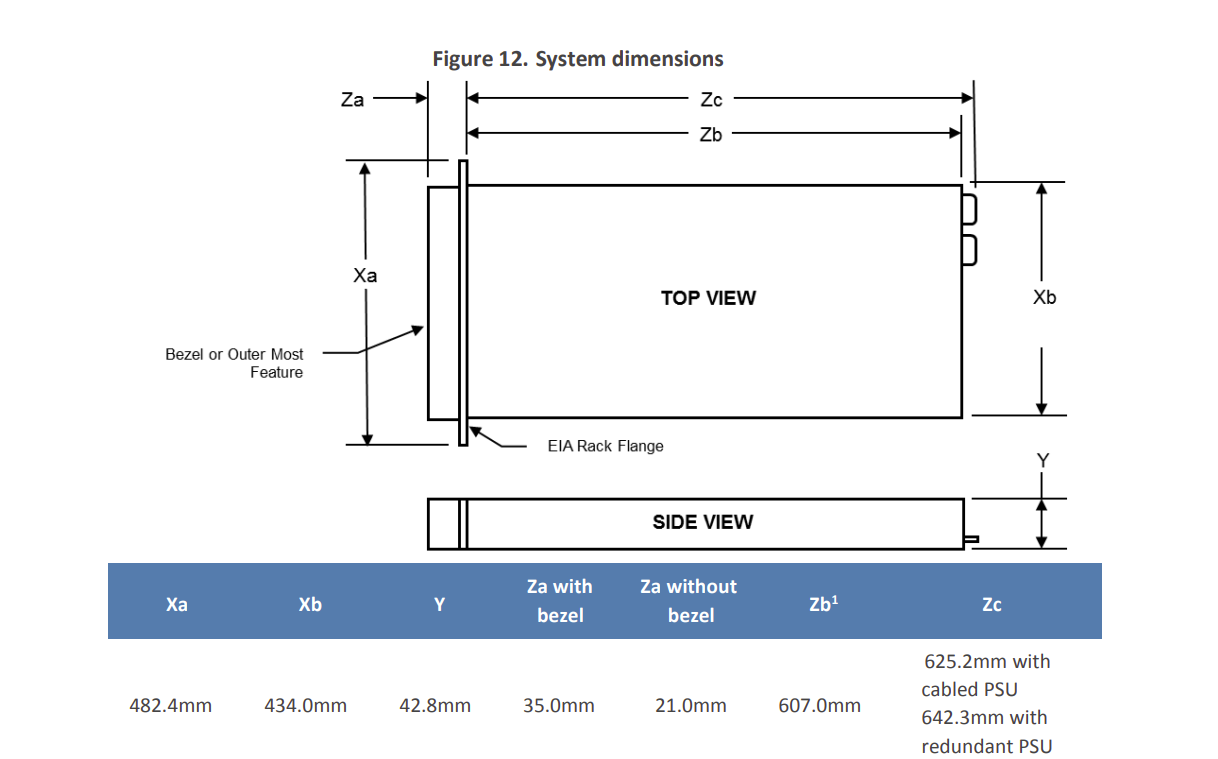
\includegraphics[width=0.5\textwidth,height=\textheight]{imatges/dimserver.png}
\caption{dimensions servidor}
\end{figure}

Cal buscar un rack que done les dimensions.

\href{https://www.dell.com/support/contents/es-es/videos/videoPlayer/os-deployment-installing-microsoft-windows-2012-r2-operating-system-by-using-lifecycle-controller/6079802988001}{video d'instal·lació}

\begin{enumerate}
\def\labelenumi{\arabic{enumi}.}
\item
  \emph{Discs durs}, admet segons documentació 4 SATA 3.5'\,' o 8 de 2.5'\,' Hot-plug. No fariem RAID per hardware. RAID: Kit RAID H710 Mini 512 MB NV (SAS/ SATA ) - 0/1/5/6/10/50/60 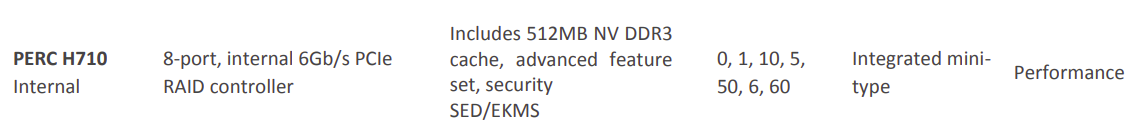
\includegraphics[width=0.8\textwidth,height=\textheight]{imatges/ser_h710.png} Caddies: 4 LFF (3.5'') incluidos

  \begin{figure}
  \centering
  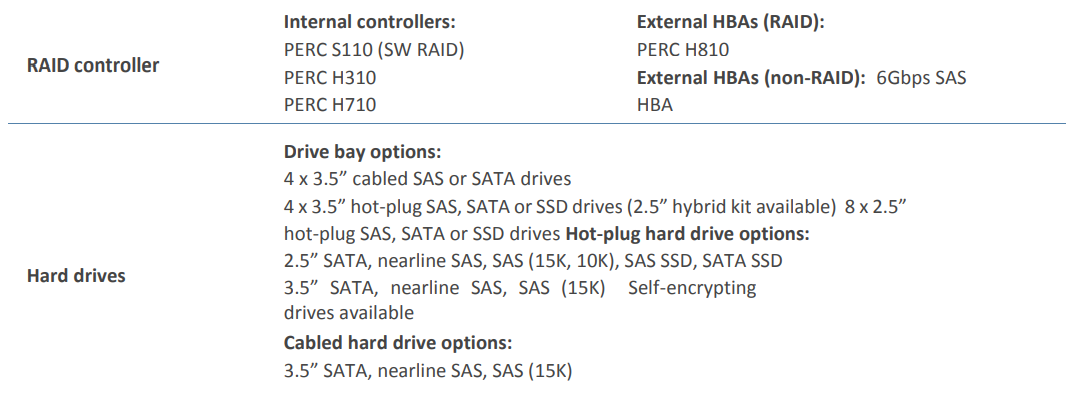
\includegraphics[width=0.8\textwidth,height=\textheight]{imatges/ser_hd.png}
  \caption{hd i Raid}
  \end{figure}

  Recomane \href{https://www.pcbox.com/st4000dm004-seagate-barracuda--st4000dm004-4000gb-3-5--serial-ata-iii/p}{SEAGATE Barracuda ST4000DM004 4000GB 3.5 Serial ATA III} \href{https://www.amazon.es/Seagate-Barracuda-Disco-Interno-cach\%C3\%A9/dp/B0713R3Y6F/ref=sr_1_5?__mk_es_ES=\%C3\%85M\%C3\%85\%C5\%BD\%C3\%95\%C3\%91\&crid=JR7AGWGKGDES\&keywords=hd\%2Bsata\%2B4tb\&qid=1651315567\&sprefix=hd\%2Bsata\%2B4tb\%2Caps\%2C93\&sr=8-5\&th=1}{amazon} \href{https://www.amazon.com/Seagate-BarraCuda-Internal-Drive-3-5-Inch/dp/B07D9C7SQH/ref=sr_1_1_sspa?keywords=4tb\%2Bsata\%2Bhard\%2Bdrive\&qid=1651315472\&sr=8-1-spons\&spLa=ZW5jcnlwdGVkUXVhbGlmaWVyPUExSldCREdJVFMzRUtNJmVuY3J5cHRlZElkPUEwNTc5NTIwMlRYQzQ0OTA0QVNDOCZlbmNyeXB0ZWRBZElkPUEwNjQxNjk2MjU1VkFSWjM1NVA4MiZ3aWRnZXROYW1lPXNwX2F0ZiZhY3Rpb249Y2xpY2tSZWRpcmVjdCZkb05vdExvZ0NsaWNrPXRydWU\&th=1}{amazon usa}

  Farien falta, 3 SATA per les dades, i un ssd 2.5 per al sistema base i les VM. Estaria bé tindre un de reserva per si falla un disc, no haver d'anar buscant un altre igual. `
\item
  RAM: RAM registrada DDR3 de 64 GB. No és la més ràpida del mercat, pero suficient per al que necessitem:

  \begin{itemize}
  \tightlist
  \item
    pfSense Min 1GB (imatge oficial), 2GB
  \item
    Znemindre NVR video 4 GB, si sobra, posar un poc mes, com anem a fer registre directe, sense detecció de moviment, no requereix tants recursos.
  \item
    Nextcloud Min 2GB, recomanat + 8GB
  \item
    Ldap, web server, antenes wifi, Collabora office server, algun altre servei futur, si es vol mail intern \ldots{} 8GB.
  \item
    Truenas, minim 8GB, quant mes millor. Les exigencies de ZFA son altes.
  \end{itemize}
\item
  CPU: 1x Intel Xeon E5-2440 V2: 8 núcleos, 16 subprocesos, 1,90 GHz (aumento de 2,40 GHz, caché de 20 MB, TDP de 95 W)
\item
  Segons la informació del venedor.

  \begin{itemize}
  \item
    Bisel: No incluido \href{https://www.pccomponentes.com/salicru-rack-rail-kit-accesorio-de-bastidor-480-a-780mm}{Rieles}: Rieles no incluidos Factor de forma: Montaje en rack 1U
  \item
    Part posterior: 1 puerto RJ-45, Preguntar si no és uno doble. En la documentacio oficial, la sèrie porta \textbf{I/O adapter options 1Gb Ethernet: Broadcom 5720 Dual Port 1Gb NIC} The Broadcom 5720 is a 14th generation 10/100/1000Base-T Ethernet LAN controller Broadcom 5720 2x1Gb Base-T 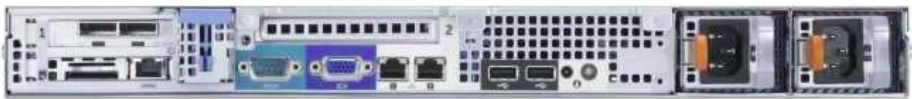
\includegraphics[width=0.6\textwidth,height=\textheight]{imatges/ser_back.png}
  \item
    2 fonts d'alimentació redundants. Fuente de alimentación: 2 fuentes de alimentación intercambiables en caliente de Dell \textbf{Platinum efficiency 350W or 550W power supply}
  \item
    Dell OpenManage Systems Management OpenManage Essentials
  \item
    Acustica, sobre 30db. El posarem en una habitació fora de l'oficina i la sala. No sera problema.
  \end{itemize}
\end{enumerate}

\hypertarget{proxmox}{%
\chapter{Proxmox}\label{proxmox}}

Instal·larem el hypervisor \href{https://www.proxmox.com/en/}{Proxmox}

Ho farem en proves viralitzant en KVM en ubuntu local, en el servidor sera directe. Per a poder importar les imatges de les iso o VM que volem instal·lar crearem un servei NFS en el host local per a poder recuperar-les i no haver d'anar en USB.

\hypertarget{preliminars}{%
\section{Preliminars}\label{preliminars}}

\hypertarget{servidor-nfs-en-local}{%
\subsection{Servidor NFS en local}\label{servidor-nfs-en-local}}

Servirem les imatges de les ISO des de el host local per no tindreles que torna a baixar. Ho farem servint un directori NFS al Guest Proxmox.

\hypertarget{en-el-host-local-installem-i-arranquem-el-servei}{%
\subsubsection{En el host local, instal·lem i arranquem el servei}\label{en-el-host-local-installem-i-arranquem-el-servei}}

Seguint la \href{https://phoenixnap.com/kb/ubuntu-nfs-server}{guia}, primer hem d'arrancar el servei

\begin{Shaded}
\begin{Highlighting}[]
\FunctionTok{sudo}\NormalTok{ apt install nfs{-}kernel{-}server}
\end{Highlighting}
\end{Shaded}

Creem la carpeta on compartirem les imatges i VM per a proxmox, canviem el propietari i els permisos.

\begin{Shaded}
\begin{Highlighting}[]
\FunctionTok{sudo}\NormalTok{ mkdir nfsdir}
\FunctionTok{sudo}\NormalTok{ chown nobody:nogroup /home/enkidu/nfs}
\FunctionTok{sudo}\NormalTok{ chmod 777 /home/enkidu/nfs}
\end{Highlighting}
\end{Shaded}

Ara exportem el recurs, editem el fitxer /etc/exports i afegim la linea per donar permisos d'accés als clients.

\begin{figure}
\centering
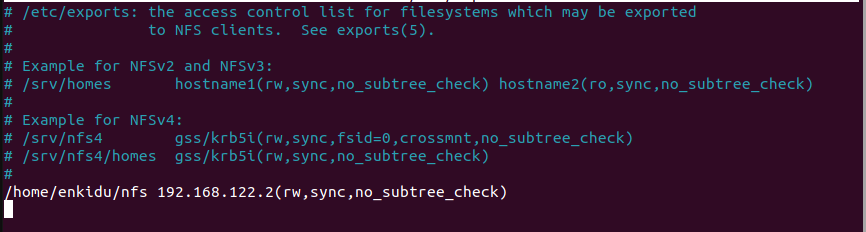
\includegraphics[width=0.8\textwidth,height=\textheight]{imatges/proxmox/nfs_imatges.png}
\caption{NFS iso i VM}
\end{figure}

Exportem el directori i reiniciem el servei

\begin{Shaded}
\begin{Highlighting}[]
\FunctionTok{sudo}\NormalTok{ exportfs }\AttributeTok{{-}a}
\FunctionTok{sudo}\NormalTok{ systemctl restart nfs{-}kernel{-}server}
\end{Highlighting}
\end{Shaded}

Ja tenim preparat el directori de les imatges per quan acabem d'instal·lar Proxmox

\hypertarget{installacio-de-proxmox-en-una-vm-amb-kvm}{%
\section{Instal·lacio de Proxmox en una VM amb KVM}\label{installacio-de-proxmox-en-una-vm-amb-kvm}}

Ho farem en KVM des de l'Ubuntu local

\begin{enumerate}
\def\labelenumi{\arabic{enumi}.}
\tightlist
\item
  Creem la VM
\item
  Elegim el medi d'instal·lacio, ho fem des d'un fitxer iso, en el servidor real, tindríem que haber fet un USB d'arrancada d'aquesta iso seguint els passos que ens indique.
\end{enumerate}

\begin{figure}
\centering
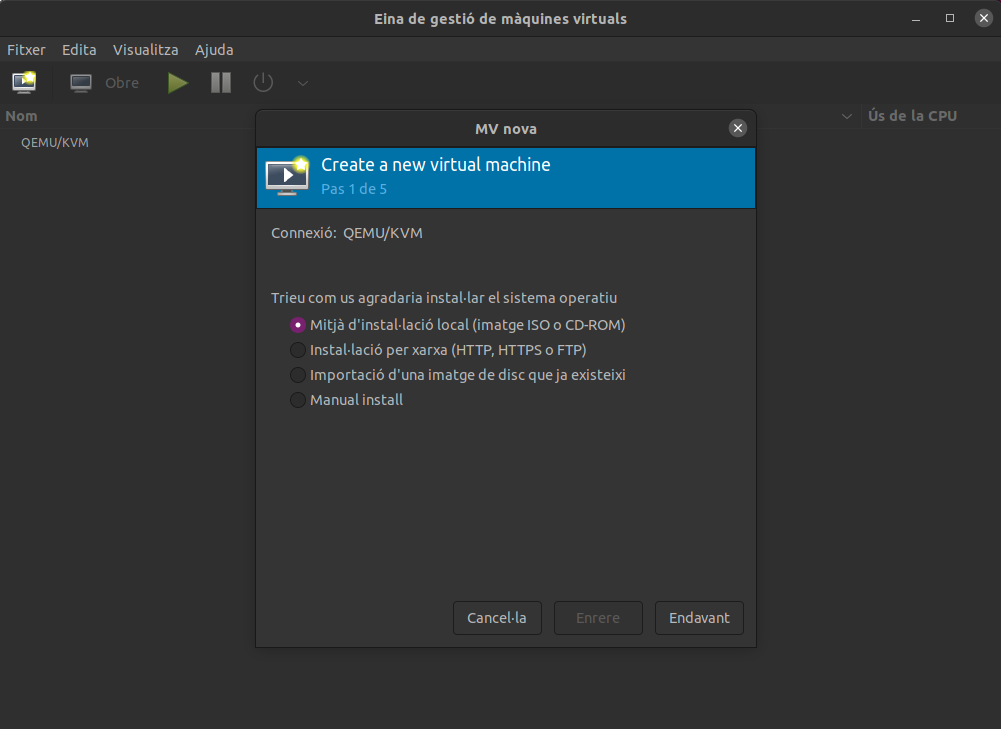
\includegraphics[width=0.5\textwidth,height=\textheight]{imatges/proxmox/proxmox_install1.png}
\caption{Crear VM en qemu}
\end{figure}

Elegim la imatge i li diguen quina es la base del SO, Debian 10

\begin{figure}
\centering
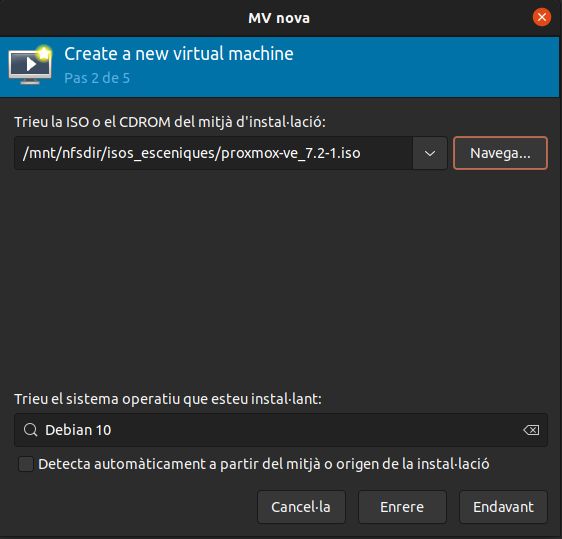
\includegraphics[width=0.5\textwidth,height=\textheight]{imatges/proxmox/proxmox_install2.png}
\caption{Elegir el fitxer iso}
\end{figure}

Creem el volum per aquesta VM, el format és qcow2 amb espai dinàmic, i la mida 40 Gib, després li afegirem un segon volum on posarem les VM. En disc ocupa 2 Gib reals, /mnt/vbox és on munte una partició del ssd en el meu portàtil, servirem d'aquest.

\begin{figure}
\centering
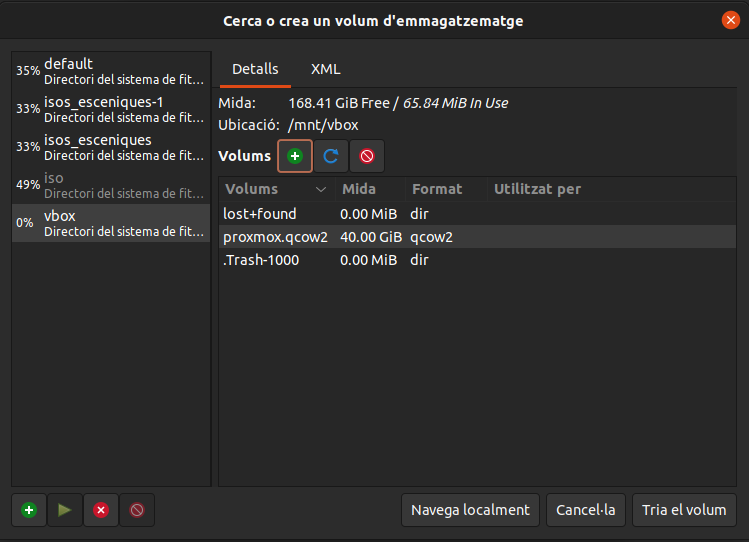
\includegraphics[width=0.5\textwidth,height=\textheight]{imatges/proxmox/proxmox_inst5.png}
\caption{Volum}
\end{figure}

Al final queda la VM com la imatge, després ja li afegirem altres HD i targetes de xara. Li he donat quasi tota la RAM, reservant part per a la host.

\begin{figure}
\centering
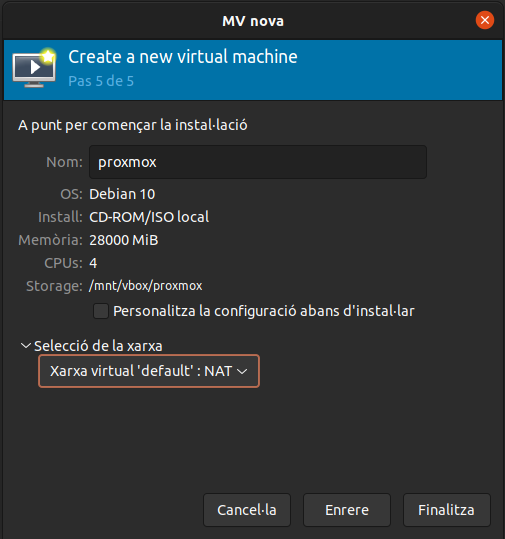
\includegraphics[width=0.5\textwidth,height=\textheight]{imatges/proxmox/proxmox_inst4.png}
\caption{VM configuració inicial}
\end{figure}

\hypertarget{arranquem-la-installacio}{%
\section{Arranquem la instal·lacio}\label{arranquem-la-installacio}}

En arrancar la VM ens ix la presentació

\begin{figure}
\centering
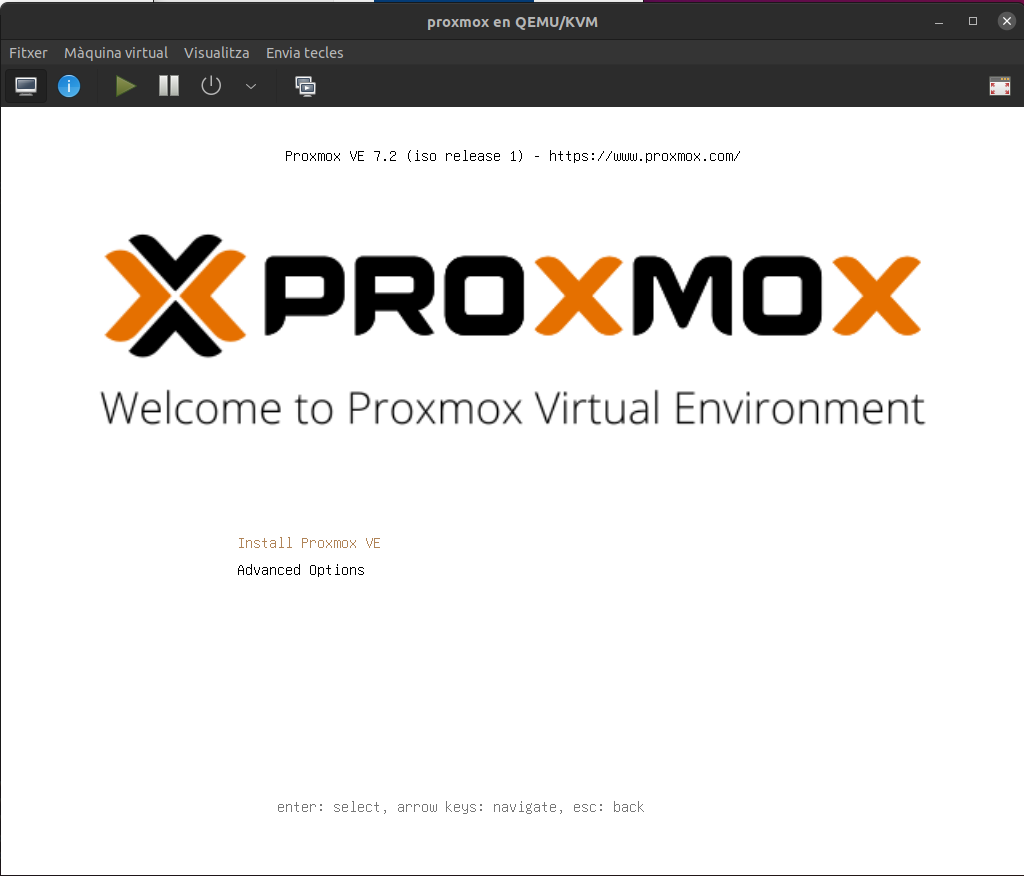
\includegraphics[width=0.5\textwidth,height=\textheight]{imatges/proxmox/proxmox_inst6.png}
\caption{presentacio proxmox}
\end{figure}

Elegim el format del HD, el podem deixar en ext4, he provat fer ZFS, per fer la prova, en el cas de tindre el servidor, es pot plantejar fer-ho amb 2 ssd RAID 1.

Pero amb una bona política de còpies de seguretat, no seria necessari.

\begin{rmdinfo}{RAID inconvenients}
Una matriu de paritat com ara RAID (1, 5, 6 o 10) introdueix cicles de treball estés i acumulació de calor reduint així la vida útil del motor. Una matriu de striping com ara RAID-0 redueix els cicles de treball i l'acumulació de calor augmentant així la vida útil del motor. També ofereix un major rendiment com a avantatge, mes velocitat de lectura i escriptura.

\end{rmdinfo}

\begin{figure}
\centering
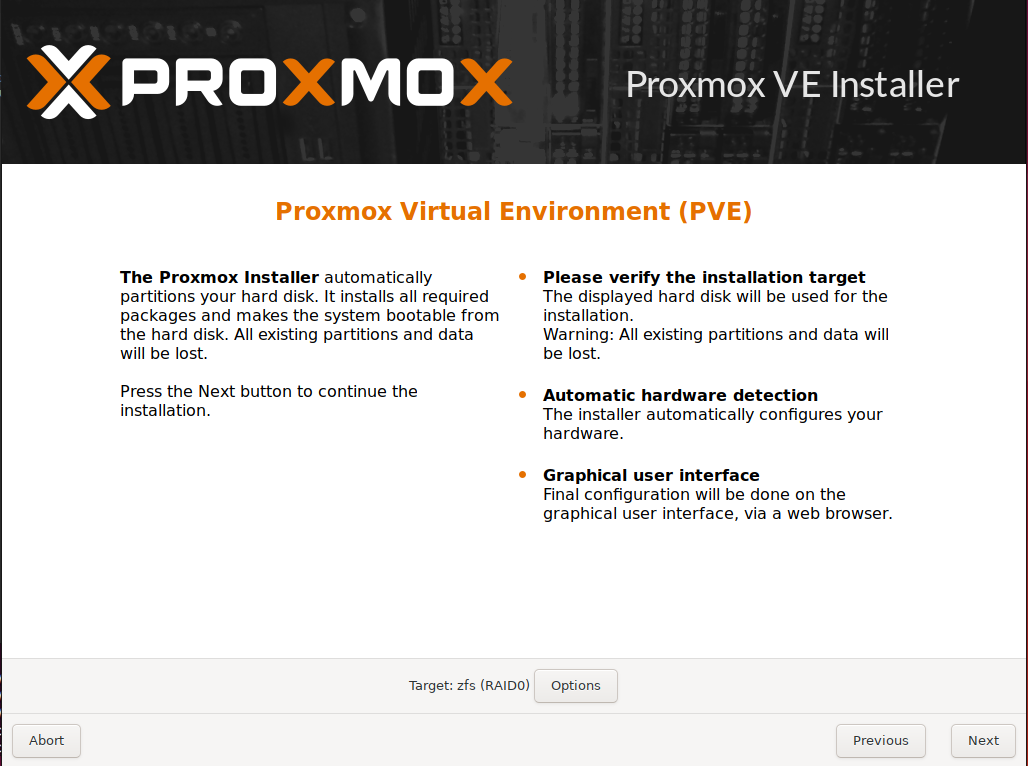
\includegraphics[width=0.5\textwidth,height=\textheight]{imatges/proxmox/proxmox_ins8.png}
\caption{configuracio HD}
\end{figure}

\begin{figure}
\centering
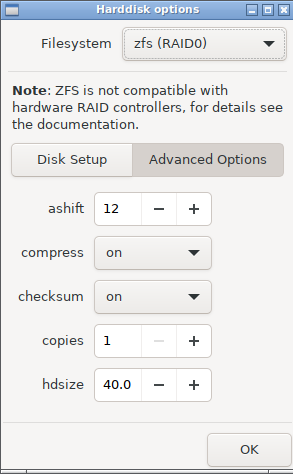
\includegraphics[width=0.2\textwidth,height=\textheight]{imatges/proxmox/proxmox_ins7.png}
\caption{Configuracio HD}
\end{figure}

Després configurem la zona horària i el password,

\begin{rmdtip}{Per entrar}
Per entrar des d'un navegador ip port 8006 amb usuari root i el password que acabem de posar.

\end{rmdtip}

\begin{figure}
\centering
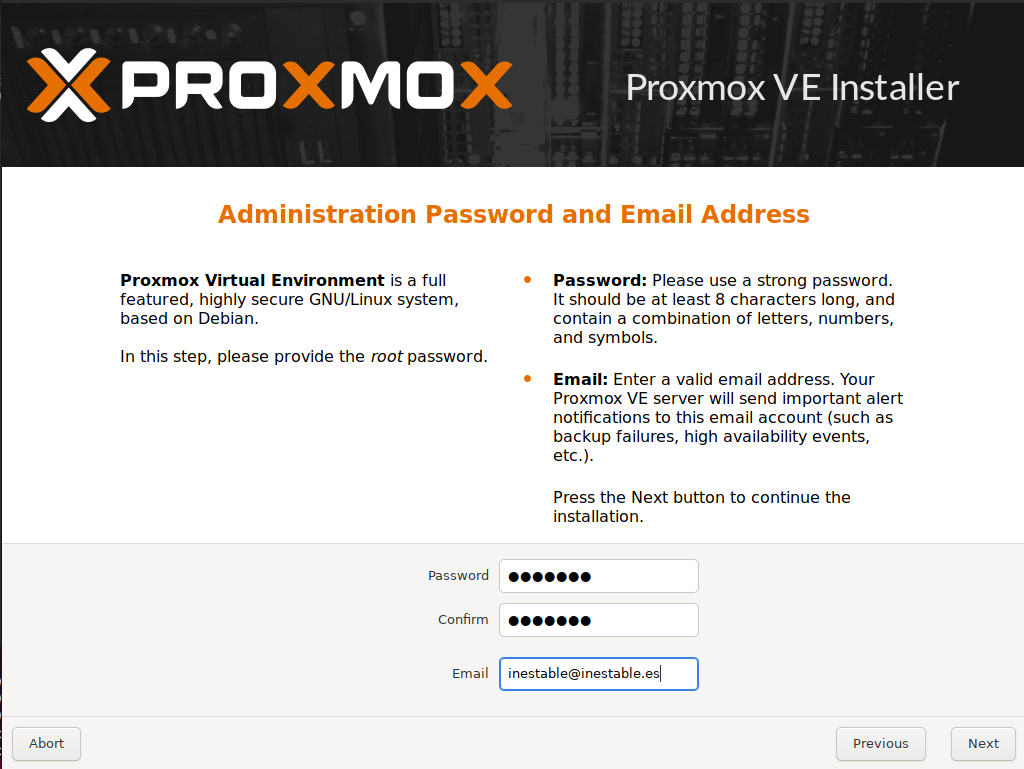
\includegraphics[width=0.5\textwidth,height=\textheight]{imatges/proxmox/proxmox_ins10.png}
\caption{passwrd}
\end{figure}

Configurem la xarxa cap a fora, internet NAT al host.

\begin{itemize}
\tightlist
\item
  Donem el FQON que sere proxmox.inestable.dedyn.io
\item
  La ip 192.168.122.2/24
\item
  El Gateway 192.168.122.1
\item
  DNS 192.168.122.1 Ho canviarem després
\end{itemize}

\begin{rmdcuidao}{directrius RFC 1918}
Triarem X.X.X.254 en pfSense tant per a la passarel·la com per a DNS perquè es troba fora dels valors predeterminats de l'interval d'adreces DHCP (192.168.x.100-192.168.x.200) a la majoria d'encaminadors. Directrius RFC 1918.

\end{rmdcuidao}

Al final queda una configuració

\begin{figure}
\centering
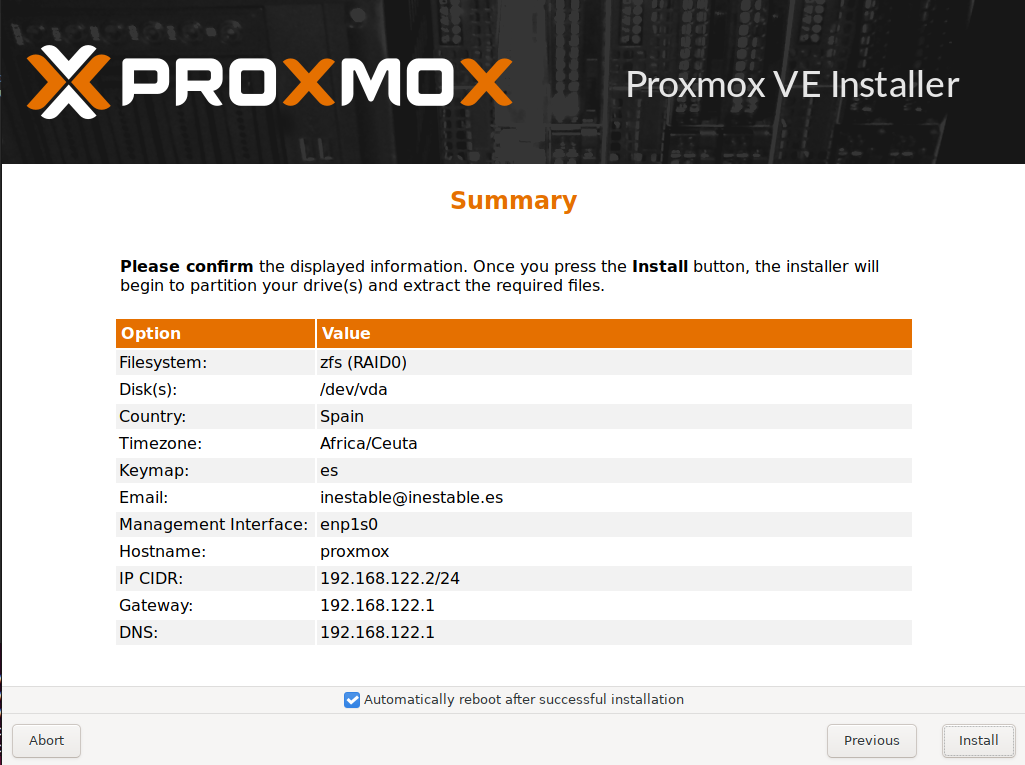
\includegraphics[width=0.5\textwidth,height=\textheight]{imatges/proxmox/proxmox_inst12.png}
\caption{configuracio final}
\end{figure}

\begin{rmdnote}{Recorda}
Canviar la Timezone després :)

\end{rmdnote}

En acabar es reinicia i passem a la configuració

\begin{figure}
\centering
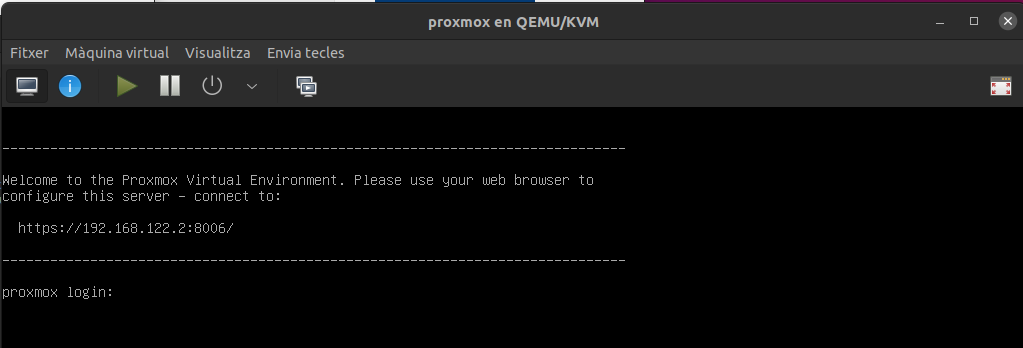
\includegraphics[width=0.5\textwidth,height=\textheight]{imatges/proxmox/proxmox_inst14.png}
\caption{Final instal·lacio}
\end{figure}

\hypertarget{primeres-configuracions}{%
\section{Primeres configuracions}\label{primeres-configuracions}}

Anem en el navegador a l'adreça IP seleccionada, al port 8006, i amb l'usuari root i el password que hem elegit, entrem.

\begin{figure}
\centering
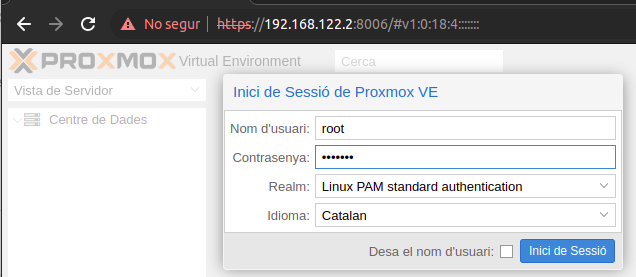
\includegraphics[width=0.6\textwidth,height=\textheight]{imatges/proxmox/proxmox_gui1.png}
\caption{proxmox gui}
\end{figure}

I ja estem dins en la primera arrencada

\begin{figure}
\centering
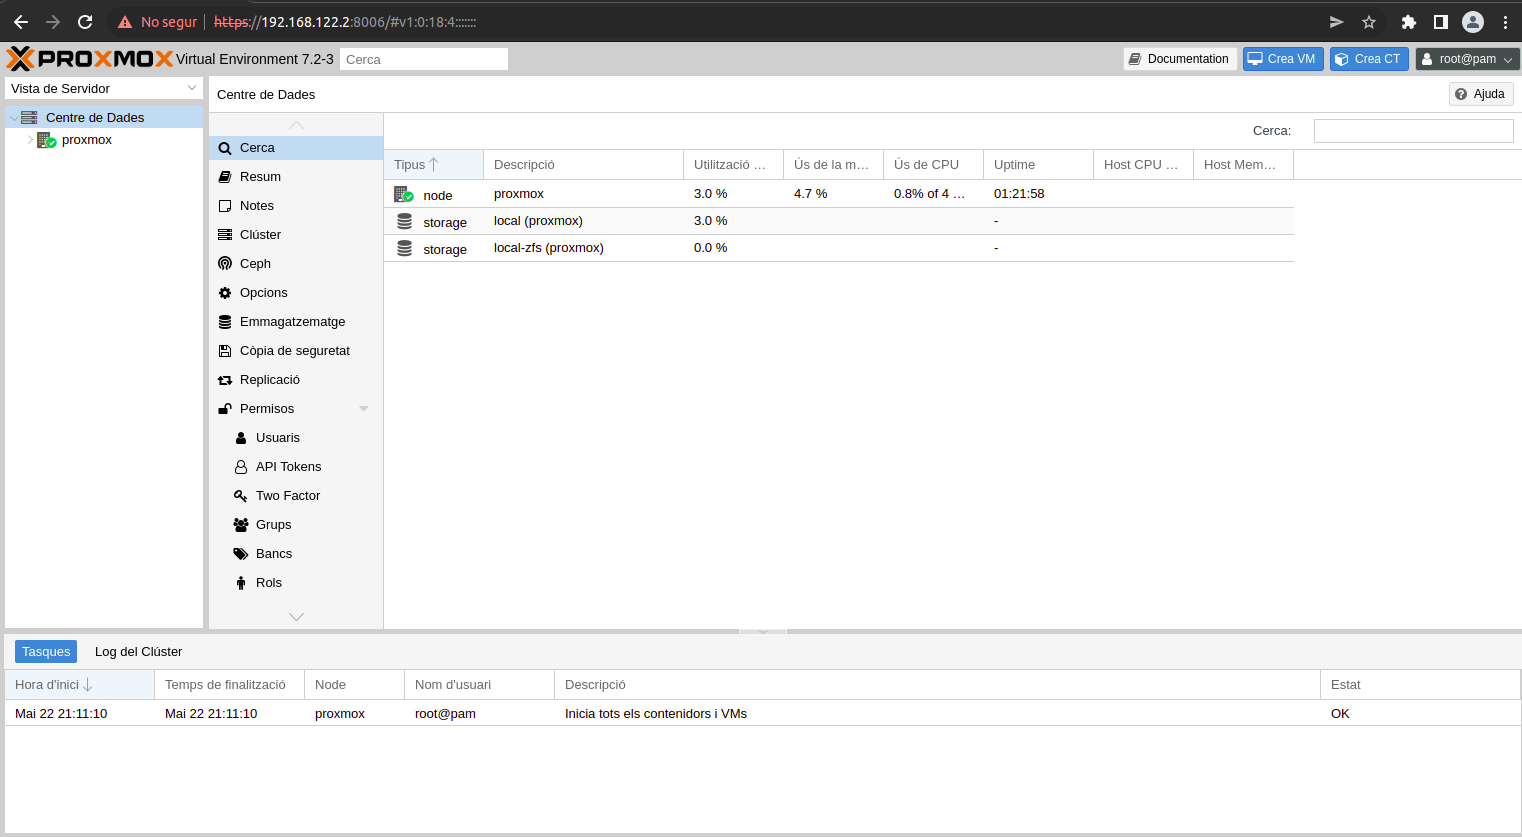
\includegraphics[width=0.8\textwidth,height=\textheight]{imatges/proxmox/proxmox_primera_arrancada.png}
\caption{Proxmox primera arrancada}
\end{figure}

Muntem el volum NFS d'abans, on tenim les ISO de les VM que volem instal.lar

Entrem per ssh en proxmox, també ho podem fer des de la GUI en la finestra del navegador.

\begin{Shaded}
\begin{Highlighting}[]
\ExtensionTok{enkidu@enkidu:/mnt/vbox$}\NormalTok{ ssh root@192.168.122.2}
\ExtensionTok{root@192.168.122.2}\StringTok{\textquotesingle{}s password: }
\StringTok{Linux proxmox 5.15.30{-}2{-}pve \#1 SMP PVE 5.15.30{-}3 (Fri, 22 Apr 2022 18:08:27 +0200) x86\_64}

\StringTok{The programs included with the Debian GNU/Linux system are free software;}
\StringTok{the exact distribution terms for each program are described in the}
\StringTok{individual files in /usr/share/doc/*/copyright.}

\StringTok{Debian GNU/Linux comes with ABSOLUTELY NO WARRANTY, to the extent}
\StringTok{permitted by applicable law.}
\StringTok{Last login: Sun May 22 22:42:06 2022 from 192.168.122.1}
\StringTok{root@proxmox:\textasciitilde{}\# }
\end{Highlighting}
\end{Shaded}

Busquem el recurs nfs on estan les ISO, la meua host te la ip 192.168.0.103 Creem un punt per enllaçar el recurs i el muntem.

\begin{Shaded}
\begin{Highlighting}[]
\ExtensionTok{root@proxmox:/mnt\#}\NormalTok{ pvesm nfsscan 192.168.0.103}
\ExtensionTok{/home/enkidu/nfs}\NormalTok{ 192.168.122.2}
\ExtensionTok{root@proxmox:\textasciitilde{}\#}\NormalTok{ mkdir }\AttributeTok{{-}p}\NormalTok{ /mnt/pvex/enkidu}
\ExtensionTok{root@proxmox:\textasciitilde{}\#}\NormalTok{ mount }\AttributeTok{{-}t}\NormalTok{ nfs 192.168.0.103:/home/enkidu/nfs /mnt/pvex/enkidu}
\ExtensionTok{root@proxmox:\textasciitilde{}\#}\NormalTok{ ls }\AttributeTok{{-}la}\NormalTok{  /mnt/pvex/enlidu}
\ExtensionTok{total}\NormalTok{ 5}
\ExtensionTok{drwxrwxrwx}\NormalTok{ 2 nobody nogroup 4096 May 22 19:54 .}
\ExtensionTok{drwxrwxrwx}\NormalTok{ 4 nobody nogroup    4 May 22 22:57 ..}
\ExtensionTok{drwxrwxrwx}\NormalTok{ 1 nobady nogroup   46 May 22 19:54 isos\_esceniques}
\ExtensionTok{drwxrwxrwx}\NormalTok{ 1 nobody nogroup   32 May 22 19:53 vm}
\end{Highlighting}
\end{Shaded}

Ho podem fer també per la GUI de proxmox. En vista de l'emmagatzemament -\textgreater{} emmagatzematge -\textgreater{} NFS Des d'aci és on es configura els tipus de discs que podem crear o afegir.

\begin{figure}
\centering
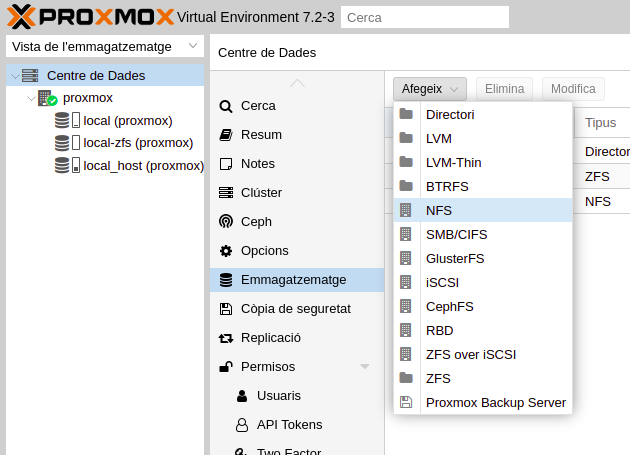
\includegraphics[width=0.5\textwidth,height=\textheight]{imatges/proxmox/proxmox_enmag.png}
\caption{Gui emmagatzematge}
\end{figure}

Ara configurem el nou recurs.

\begin{figure}
\centering
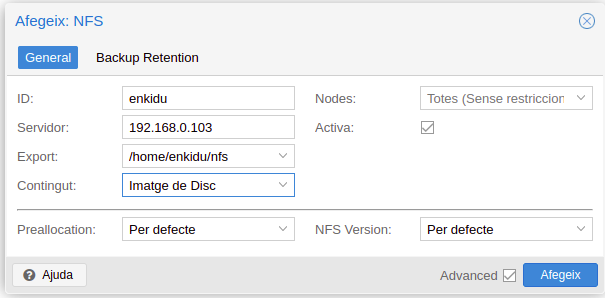
\includegraphics[width=0.5\textwidth,height=\textheight]{imatges/proxmox/proxmox_emn2.png}
\caption{Muntar NFS}
\end{figure}

\begin{enumerate}
\def\labelenumi{\arabic{enumi}.}
\tightlist
\item
  Li donem un ID, que sera també el nom de la carpeta que es crea en /mnt/vpex/per muntar el recurs.
\item
  La IP o FQON on està el recurs. Com encara no tenim DNS, li posem la IP.
\item
  El directori compartit, al posar la IP, en el menu desplegable ens mostra els recursos compartits per aquest servidor NFS.
\item
  El tipus de recurs que es comparteix. Volem guardar aci les imatges ISO, podem seleccionar altres recursos com copies de seguretat, Discs VM \ldots{}
\item
  Afegim
\end{enumerate}

I ja tindríem el recurs accessible.

\begin{figure}
\centering
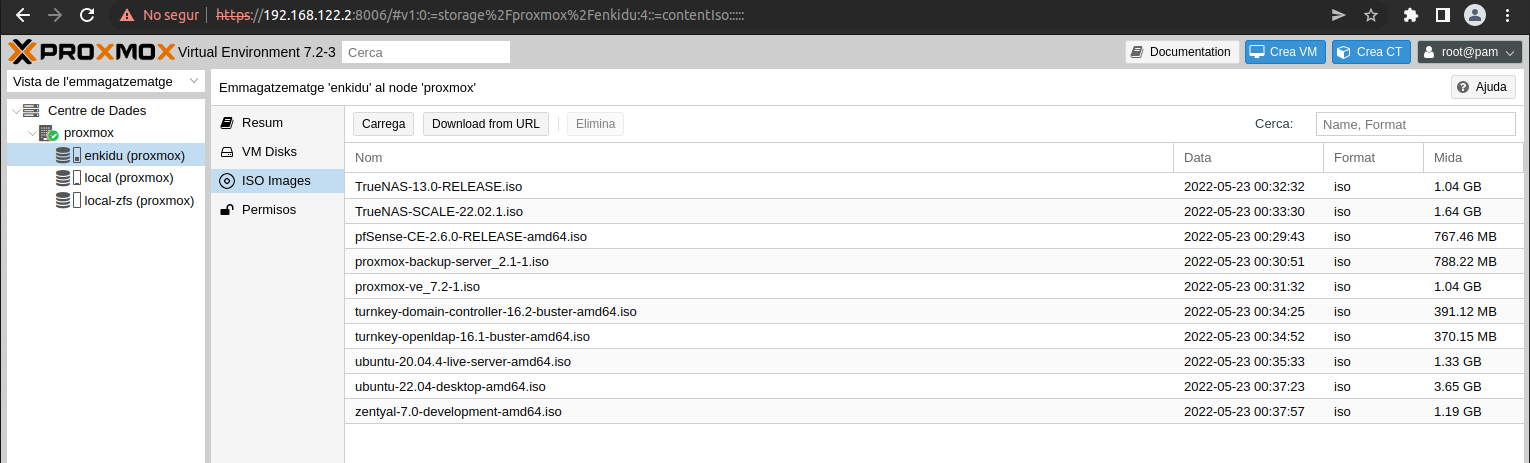
\includegraphics[width=0.8\textwidth,height=\textheight]{imatges/proxmox/proxmox_enm4.png}
\caption{Recurs NFS}
\end{figure}

Ja podríem començar a crear les VM en el volum local dins la VM, pero primer afegirem un nou HD, per tindre separat el sistema host de les VM, es com si ara li posarem un altre HD ssd al servidor, ho recomana la documentació oficial per més estabilitat. En la pràctica, segurament tindrem un sol ssd per al proxmox i les VM. Faríem les particions abans una per al sistema base i l'altra per a les VM, en el cas de tindre dos SSD, faríem un RAID1 (espill) + ZFS, i el mateix una partició separada de l'arrel per a posar les VM. En gestió personalitzada dels dics.

\begin{rmdwarn}{No per Maquinari}
Per fer el RAID1 no el faríem des del maquinari del servidor el servidor no es nou, i si fallara, haguérem de buscar la mateixa peça perquè arranque, el format ZFS no es compatible amb RAID per maquinari, ja porta el seu propi sistema de fer-ho.

\end{rmdwarn}

\hypertarget{actualitzar-repositoris}{%
\section{Actualitzar repositoris}\label{actualitzar-repositoris}}

Per defecte els repositoris que porta definits es la versió enterprise, que s'ha de tindre subscriptcio per poder accedir, canciarem per la No-Subscription Repository

\href{https://pve.proxmox.com/wiki/Package_Repositories}{Documentacio}

En /etc/apt/source.list afegim i el repositori No-Subscription commentem l'enterprise

\begin{Shaded}
\begin{Highlighting}[]
\ExtensionTok{deb}\NormalTok{ http://ftp.debian.org/debian bullseye main contrib}
\ExtensionTok{deb}\NormalTok{ http://ftp.debian.org/debian bullseye{-}updates main contrib}

\CommentTok{\# PVE pve{-}no{-}subscription repository provided by proxmox.com,}
\CommentTok{\# NOT recommended for production use}
\ExtensionTok{deb}\NormalTok{ http://download.proxmox.com/debian/pve bullseye pve{-}no{-}subscription}

\CommentTok{\# security updates}
\ExtensionTok{deb}\NormalTok{ http://security.debian.org/debian{-}security bullseye{-}security main contrib}
\end{Highlighting}
\end{Shaded}

\hypertarget{afegir-nous-hd-al-servidor}{%
\section{Afegir nous HD al servidor}\label{afegir-nous-hd-al-servidor}}

Ara seria el moment que afegiríem els HD al servidor físic. El cas hipotètic seria tindre 3 HD SATA i un ssd.

Tots els discs es formataran fent servir ZFS pels avantatges que proporciona, instantànies, control d'errors, redimensionament de volums, compressió nativa \ldots{}

El que es proposa

\begin{enumerate}
\def\labelenumi{\arabic{enumi}.}
\item
  El SSD siga d'us exclusiu de Proxmox, una partició per al sistema base i l'altra per guardar les VM dels serveis. I els SATA per ús exclusiu de Truenas, i des d'aci compartir volums en la resta de VM, tenint centralitzada l'emmagatzemament de dades facilitant les còpies de seguretat.
\item
  Els SATA es dividiran en dos blocs, SATA 1 i 2 format un RAID 0 que ens proporciona millor rendiment de velocitat, on crearem espai compartit per NFS per:

  \begin{itemize}
  \tightlist
  \item
    Dades d'usuaris Nextcloud.
  \item
    Còpies de seguretat de les VM, fitxers de configuració, repositori ISO dels sistemes a instal·lar, part administrativa.
  \item
    Espai per la captura de video, en dues seccions, una per a videos editats per guardar, i l'altra per a registres en brut.
  \item
    Altres serveis futurs, com un xicotet espai per al servidor web de promocions internes, que podria estar dins de l'espai de Nextcloud per poder editar des d'aques entorn el contingut (configuració amb \href{https://picocms.org}{pico}), o espai per contingut Wordpress si s'adopta aquesta opció.
  \end{itemize}
\item
  L'altre SATA per fer còpies de seguretat.

  \begin{itemize}
  \tightlist
  \item
    De les dades de Nextcloud.
  \item
    De les còpies de seguretat de Proxmox i fitxers administratius.
  \item
    De la carpeta de Video de còpies per guardar. Soles els arxius de video d'obres pròpies.
  \end{itemize}
\end{enumerate}

\begin{rmdtip}{Tip}
Per la forma en què l'empresa vol d'utilització les còpies de video, fer captures de video per a les companyies convidades per oferir-les com un servei mes de la sala, aquestes còpies s'esborraran una vegada el convidat la descarregue. I les pròpies s'han d'editar. No val la pena estar gastant gran quantitat de recursos del servidor en fer un RAID 1, quan el pes més gran de les dades son descartables. Amb una política frequent rsync entre volums en Truenas, les tindrem protegides amb poc consum.

\end{rmdtip}

\begin{figure}
\centering
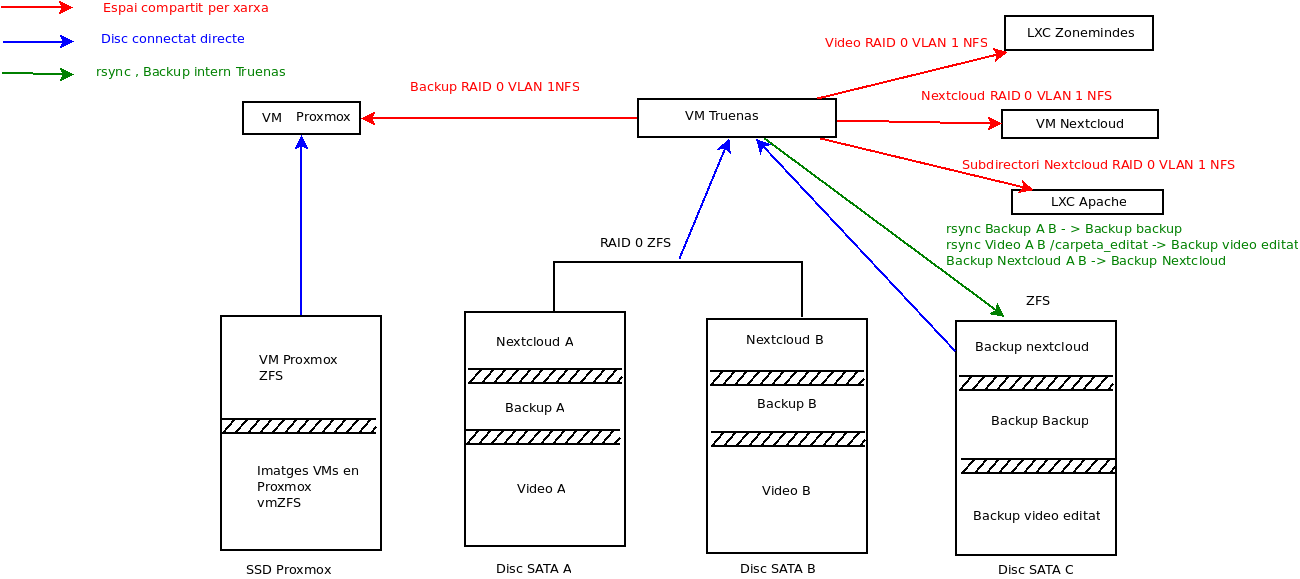
\includegraphics{imatges/proxmox/Discs_servidor.png}
\caption{Discs en el servidor}
\end{figure}

\hypertarget{procediment}{%
\subsection{Procediment}\label{procediment}}

Simularem que li afegim un nou SSD de 100Gib i tres SATA dos de 50 Gib i un de 100 Gib. Creem els 4 volums en format qcow2 i els afegim en KVM a la VM de Proxmox

En KVM/qemu creem els discs i els afegim a la nostra VM.

\begin{figure}
\centering
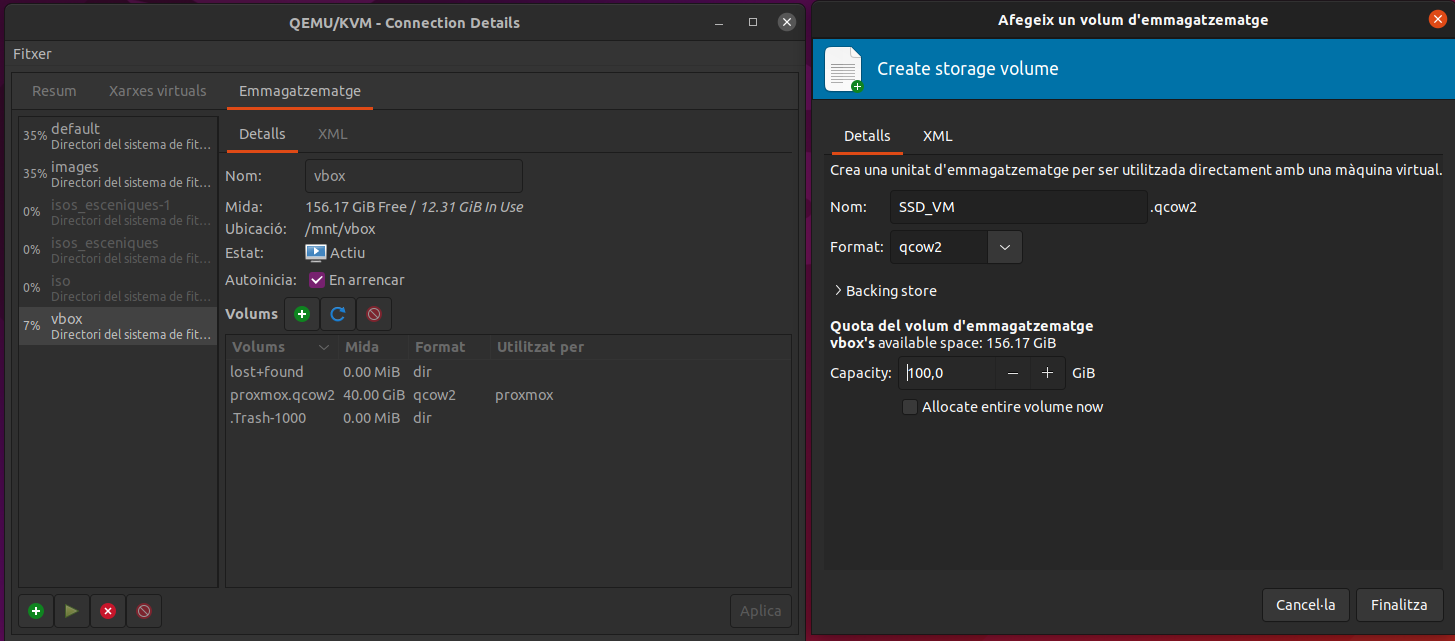
\includegraphics[width=0.8\textwidth,height=\textheight]{imatges/proxmox/proxmox_SSD.png}
\caption{Proxmox afegir SSD per a VM}
\end{figure}

\begin{figure}
\centering
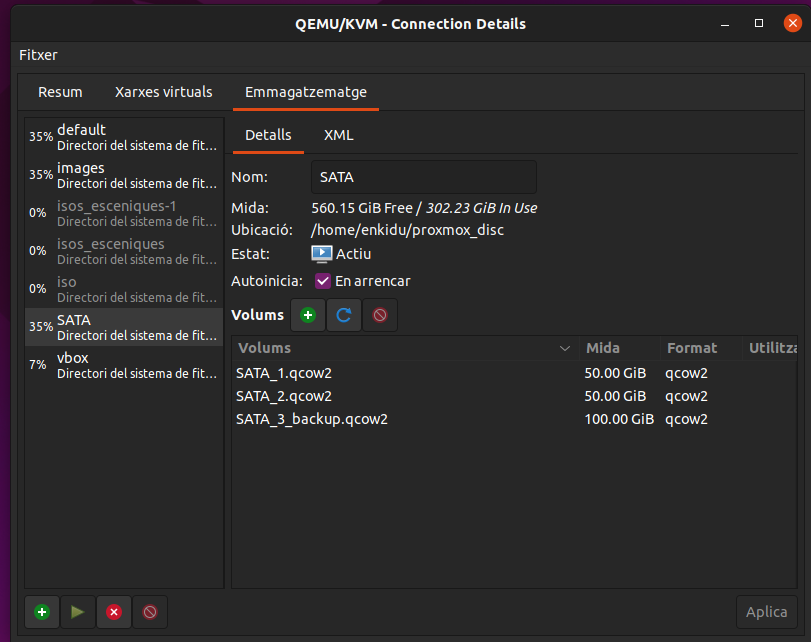
\includegraphics[width=0.5\textwidth,height=\textheight]{imatges/proxmox/proxmox_SATA.png}
\caption{Proxmox SATA}
\end{figure}

Afegim els discs, com a VirtiO. Ho farem primer soles en el SSD i després posarem els altres.

\begin{figure}
\centering
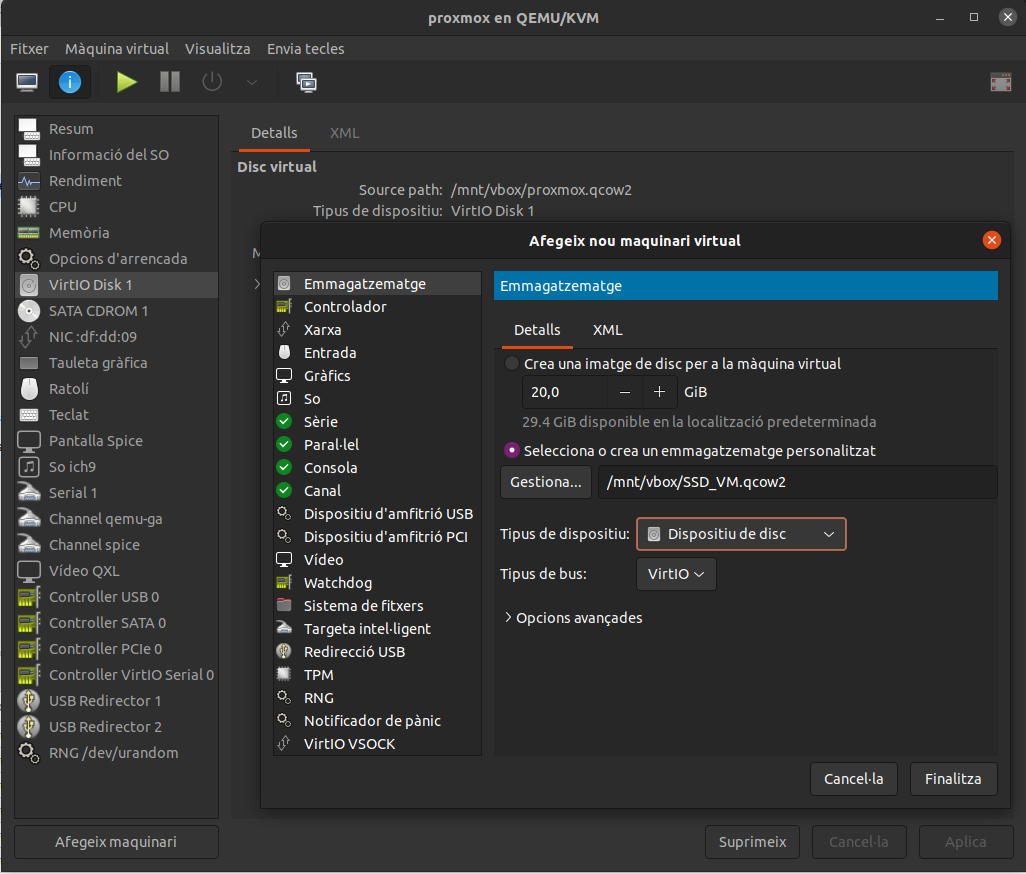
\includegraphics[width=0.5\textwidth,height=\textheight]{imatges/proxmox/proxmov_af_ssd.png}
\caption{Proxmox afegir SSD}
\end{figure}

Arranquem. i apareix el nou HD /dev/vdb

\begin{figure}
\centering
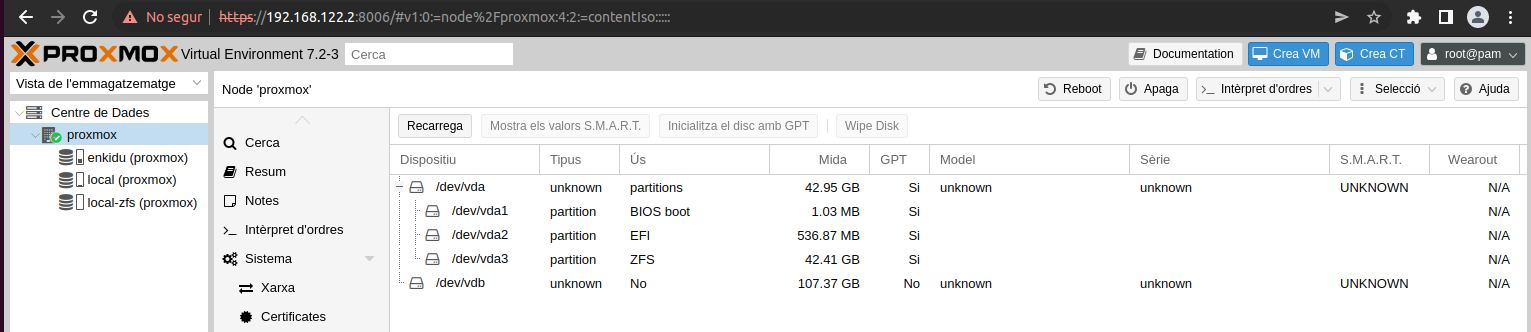
\includegraphics[width=0.8\textwidth,height=\textheight]{imatges/proxmox/proxmox_nou_ssd.png}
\caption{SSD}
\end{figure}

\hypertarget{configuracio-del-nou-ssd-per-a-les-vm}{%
\subsection{Configuracio del nou SSD per a les VM}\label{configuracio-del-nou-ssd-per-a-les-vm}}

Tenim dues opcions, configurar el nou volum com a LVM-thin o com un volum ZFS

\begin{enumerate}
\def\labelenumi{\arabic{enumi}.}
\tightlist
\item
  Si el volguérem configurar com a LVM \href{https://pve.proxmox.com/wiki/Logical_Volume_Manager_(LVM)}{Documentacio}
\end{enumerate}

\begin{Shaded}
\begin{Highlighting}[]
\ExtensionTok{root@proxmox:\textasciitilde{}\#}\NormalTok{ cat /proc/partitions }
\ExtensionTok{major}\NormalTok{ minor  }\CommentTok{\#blocks  name}

 \ExtensionTok{252}\NormalTok{        0   41943040 vda}
 \ExtensionTok{252}\NormalTok{        1       1007 vda1}
 \ExtensionTok{252}\NormalTok{        2     524288 vda2}
 \ExtensionTok{252}\NormalTok{        3   41417711 vda3}
 \ExtensionTok{252}\NormalTok{       16  104857600 vdb}
  \ExtensionTok{11}\NormalTok{        0    1048575 sr0}
\end{Highlighting}
\end{Shaded}

Crearem un LVM per al nou SSD que acabem d'instal·lar, aquesta opció te tots els avantatges de LVM, podem afegir mes espai si en el futur ens fera falta, afegint un nou ssd, canviar la mida de les VM \ldots{}

Per consola, primer crear el volum, soles tenim un i després el grup de volums que li direm lvsVM es per a imatges de màquines virtuals.

\begin{Shaded}
\begin{Highlighting}[]
\ExtensionTok{root@proxmox:\textasciitilde{}\#}\NormalTok{ pvcreate /dev/vdb}
  \ExtensionTok{Physical}\NormalTok{ volume }\StringTok{"/dev/vdb"}\NormalTok{ successfully created.}
\ExtensionTok{root@proxmox:\textasciitilde{}\#}\NormalTok{ vgcreate lvmVM /dev/vdb}
  \ExtensionTok{Volume}\NormalTok{ group }\StringTok{"lvmVM"}\NormalTok{ successfully created}
\end{Highlighting}
\end{Shaded}

També ho podem fer per la GUI, els mateixos passos que farem després en el format ZFS pero elegint LVM

Afegim el volum logic

\begin{Shaded}
\begin{Highlighting}[]
\ExtensionTok{root@proxmox:\textasciitilde{}\#}\NormalTok{ lvcreate }\AttributeTok{{-}n}\NormalTok{ VM }\AttributeTok{{-}V}\NormalTok{ 100G lvmVM/lvmVM}
  \ExtensionTok{WARNING:}\NormalTok{ Sum of all thin volume sizes }\ErrorTok{(}\ExtensionTok{100.00}\NormalTok{ GiB}\KeywordTok{)} \ExtensionTok{exceeds}\NormalTok{ the size of thin pool}
  \ExtensionTok{lvmVM/lvmVM}\NormalTok{ and the size of whole volume group }\ErrorTok{(}\OperatorTok{\textless{}}\NormalTok{100.00 }\ExtensionTok{GiB}\KeywordTok{)}\BuiltInTok{.}
  \ExtensionTok{WARNING:}\NormalTok{ You have not turned on protection against thin pools running out of space.}
  \ExtensionTok{WARNING:}\NormalTok{ Set activation/thin\_pool\_autoextend\_threshold below 100 to trigger}
  \ExtensionTok{automatic}\NormalTok{ extension of thin pools before they get full.}
  \ExtensionTok{Logical}\NormalTok{ volume }\StringTok{"VM"}\NormalTok{ created.}
\end{Highlighting}
\end{Shaded}

En aquest tipus de volums l'hauríem de configurar com a LVM-thin si el volem utilitzar per a emmagatzemament d'imatges, ofereix un suport eficient per a instantànies i clons. És la forma predeterminada de particions de Proxmos per a les VM que genera en el volum local, fa una part per al sistema base i una altra que li diu local per a les VM, és el que es veu en el disc /dev/vda.

\begin{enumerate}
\def\labelenumi{\arabic{enumi}.}
\setcounter{enumi}{1}
\tightlist
\item
  Com a volum ZFS
\end{enumerate}

Al final el creem com a ZFS, que té les mateixes característiques que LVM-thin millorades.

Dins de discs elegim ZFS -\textgreater{} afegir, seleccionem el disc que volem crear, apareixen els nous discs afegits. El /dev/vde és el ssd de 100G que configurarem.

\begin{figure}
\centering
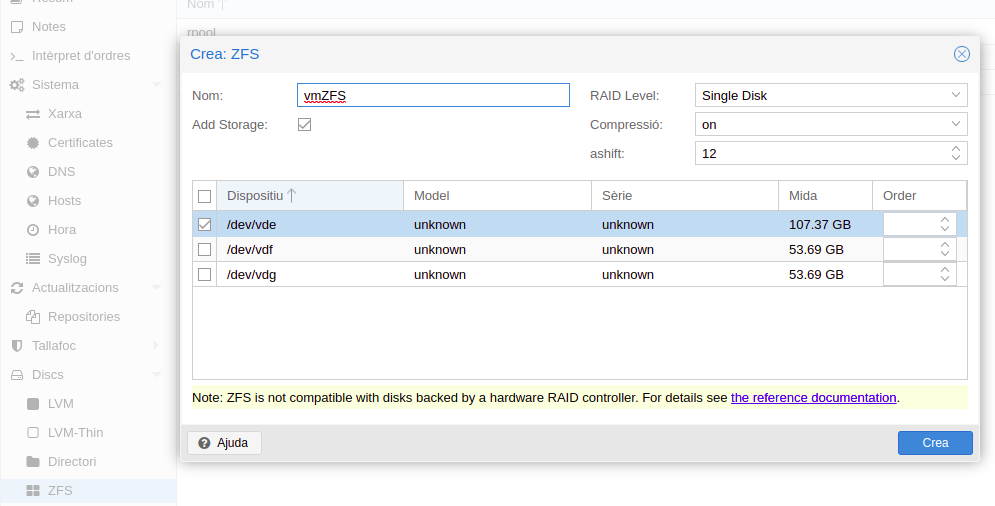
\includegraphics[width=0.5\textwidth,height=\textheight]{imatges/proxmox/vmZFS_disc.png}
\caption{Crear disc VM}
\end{figure}

El crearia i l'afegeix com a nou emmagatzemament

El podem editar i li diguem que tipus de contingut volem que es guarde en ell, Imatges de disc i contenidors.

\begin{figure}
\centering
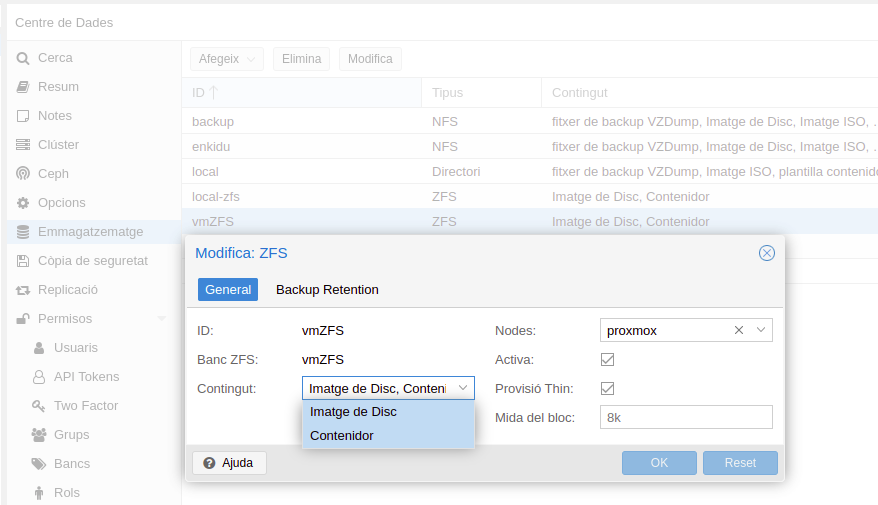
\includegraphics[width=0.5\textwidth,height=\textheight]{imatges/proxmox/ZFS_VM.png}
\caption{vmZFS per VM i contenidors}
\end{figure}

Ja el podríem utilitzar per crear la primera VM i guardar-la dins d'ell.

\hypertarget{afegir-lemmagatzenament-de-cuxf2pia-de-seguretat}{%
\section{Afegir l'emmagatzenament de còpia de seguretat}\label{afegir-lemmagatzenament-de-cuxf2pia-de-seguretat}}

Una vegada creat i compartit el volum de còpia de seguretat, en la secció de Truenas, l'afegim a emmagatzemaments. Aquest volum l'hem compartit com a NFS + ZFS, ho fem com en el cas del disc de la host -\textgreater{} afegir NFS, pero ara li direm que guarde en tipus de dades, elegim totes. Aci guardarem tant les ISO, les VM, els contenidors que baixem\ldots{} sera d'on en un futur obtindrem els recursos d'administració, eliminant l'espai compartit de la host d'on importem ara les ISO per instal·lar les VM.

\begin{figure}
\centering
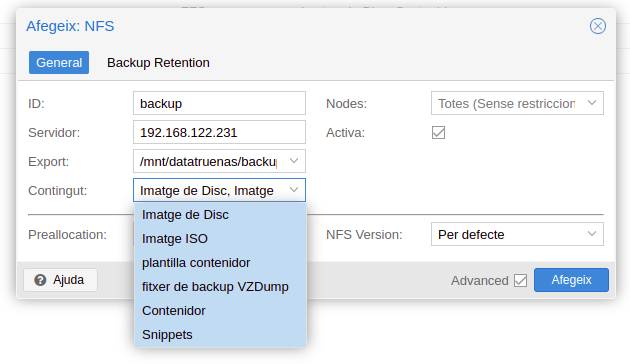
\includegraphics[width=0.5\textwidth,height=\textheight]{imatges/proxmox/tipus_disk_backup.png}
\caption{Afegir HD NFS Backup}
\end{figure}

Ja tindríem el nou espai backup

\hypertarget{crear-nova-vm}{%
\section{Crear nova VM}\label{crear-nova-vm}}

Crearem una nova VM Truenas per definir els passos a seguir.

\begin{enumerate}
\def\labelenumi{\arabic{enumi}.}
\tightlist
\item
  Creem una nova VM, elegim el node, soles tenim un proxmox
\item
  L'ID, es com reconeix Proxmox la VM
\item
  Li donem un nom
\end{enumerate}

\begin{figure}
\centering
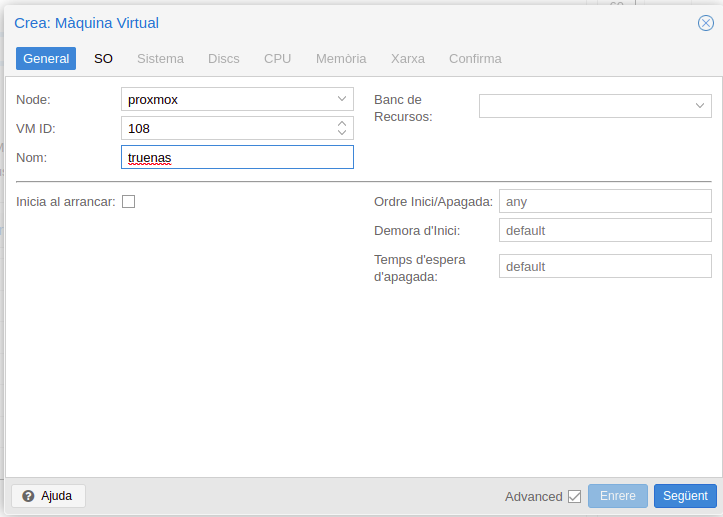
\includegraphics[width=0.5\textwidth,height=\textheight]{imatges/proxmox/install_truenas1.png}
\caption{Nova VM truenas}
\end{figure}

\begin{enumerate}
\def\labelenumi{\arabic{enumi}.}
\setcounter{enumi}{3}
\tightlist
\item
  Elegim el SO, li diguem el lloc on està la imatge, de moment, del recurs compartit en la host, més avant seria el recurs Backup d'administracio en Truenas.
\item
  Elegim de les ISO disponibles la que volem
\item
  Elegim el tipus de sistema a instal·lar, Linux
\end{enumerate}

\begin{figure}
\centering
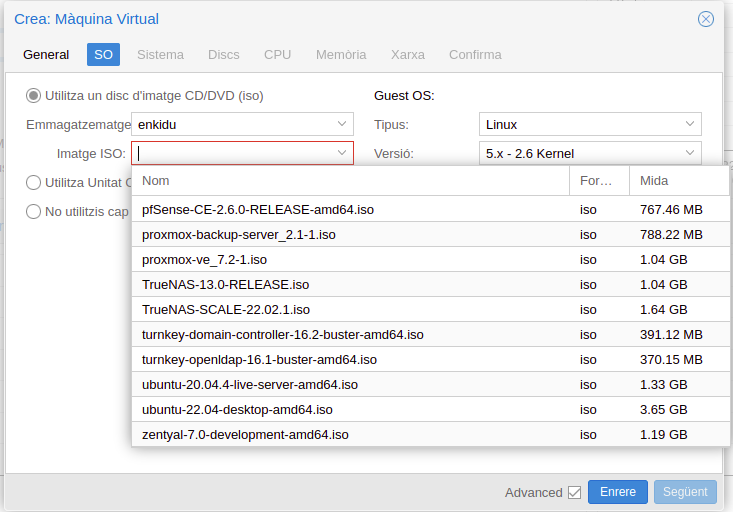
\includegraphics[width=0.5\textwidth,height=\textheight]{imatges/proxmox/install_truenas2.png}
\caption{Nova VM truenas}
\end{figure}

\begin{enumerate}
\def\labelenumi{\arabic{enumi}.}
\setcounter{enumi}{6}
\tightlist
\item
  Podríem elegir targeta gràfica, en la que ve per defecte ens va be, Si la VM requerira potència GPU i el servidor disposara, la podríem configurar.
\item
  El tipus d'emulacio del procesador.
\end{enumerate}

\begin{figure}
\centering
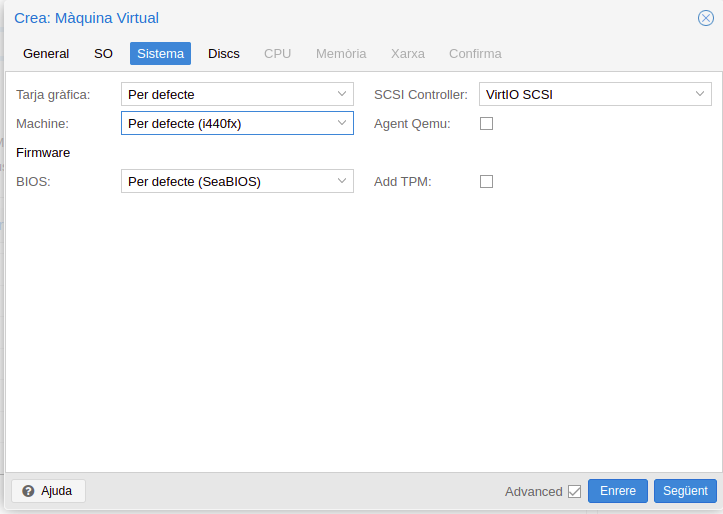
\includegraphics[width=0.5\textwidth,height=\textheight]{imatges/proxmox/install_truenas3.png}
\caption{Nova VM truenas}
\end{figure}

\begin{enumerate}
\def\labelenumi{\arabic{enumi}.}
\setcounter{enumi}{8}
\tightlist
\item
  Definim el tipus de disc SATA
\item
  On es creara la VM, en l'espai que hem configurat per aquesta tasca vmZFS
\item
  La grandària del disc
\item
  El format, per caracteristique del lloc on creem les VM, soles ens deixa elegir el format RAW, pero en ser ZFS i l'hem definit la compressio, és millor que un volum qcow2, té accés directe al disc va més fluid, i mantenim la mida dinamica.
\end{enumerate}

\begin{figure}
\centering
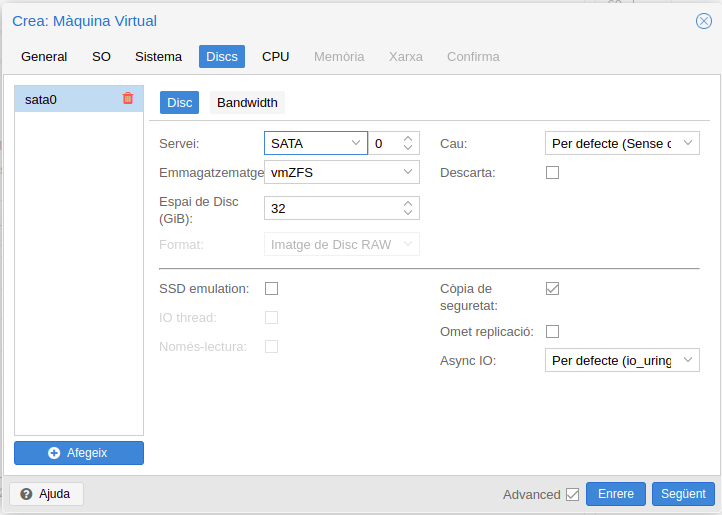
\includegraphics[width=0.5\textwidth,height=\textheight]{imatges/proxmox/install_truenas4.png}
\caption{Nova VM truenas}
\end{figure}

\begin{enumerate}
\def\labelenumi{\arabic{enumi}.}
\setcounter{enumi}{12}
\tightlist
\item
  Configurariem el número de CPU
\end{enumerate}

\begin{figure}
\centering
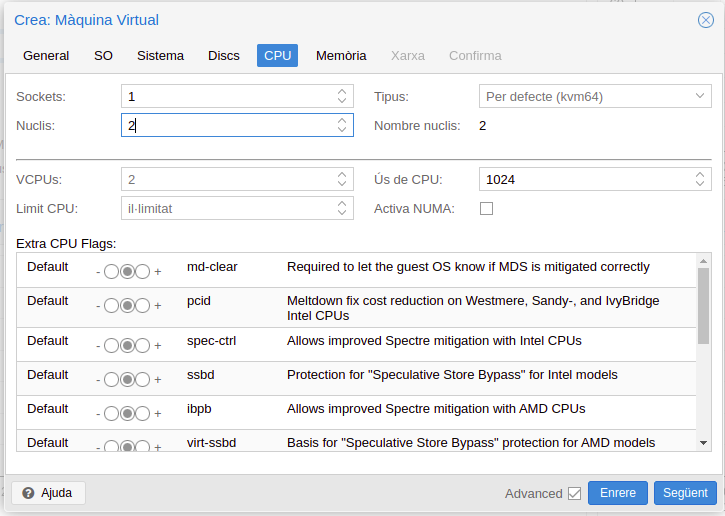
\includegraphics[width=0.5\textwidth,height=\textheight]{imatges/proxmox/install_truenas5.png}
\caption{Nova VM truenas}
\end{figure}

\begin{enumerate}
\def\labelenumi{\arabic{enumi}.}
\setcounter{enumi}{13}
\tightlist
\item
  La memoria, Elegim la maxima que pot utilitzar
\item
  Per la forma de gestionar la memoria, li podem definir la minima, si no l'utilitza, no reserva tota la que li hem donat, soles la minima, alliberant la resta al sistema.
\item
  Comparticions, crec recordar que és un mòdul del nucli linux, que comparteix memoria amb altres VM, aquesta és una FreeBSD, les llibreries igual amb una altra FreeBSD les comparteixen, alliberant memoria.
\end{enumerate}

\begin{figure}
\centering
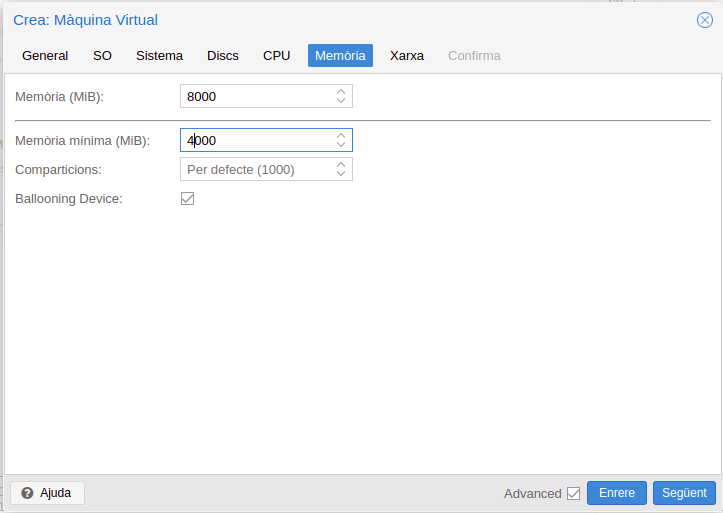
\includegraphics[width=0.5\textwidth,height=\textheight]{imatges/proxmox/install_truenas6.png}
\caption{Nova VM truenas}
\end{figure}

\begin{enumerate}
\def\labelenumi{\arabic{enumi}.}
\setcounter{enumi}{16}
\tightlist
\item
  La Xarxa, de moment per a les primeres configuracions la posem en el pont vmbr0, és el pont NAT a la host, després editarem la configuracio de la VM i la posarem en el pont Open virtual switch, en les VLAN que volem que estiga, afegint-li més targetes de xarxa.
\end{enumerate}

\begin{figure}
\centering
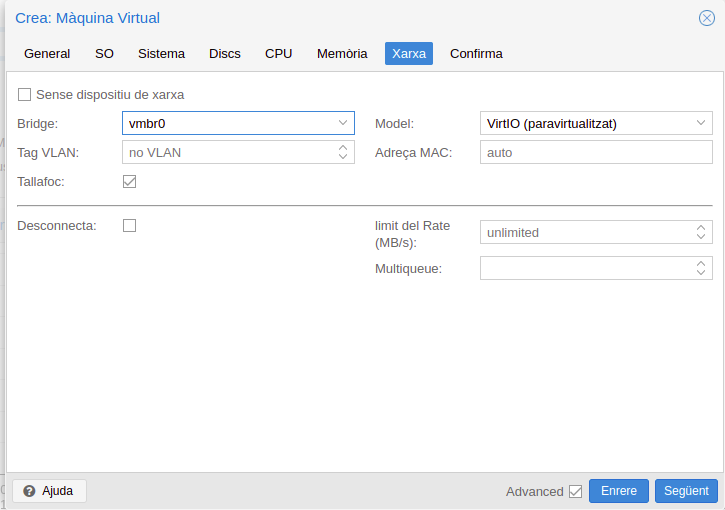
\includegraphics[width=0.5\textwidth,height=\textheight]{imatges/proxmox/install_truenas7.png}
\caption{Nova VM truenas}
\end{figure}

\begin{enumerate}
\def\labelenumi{\arabic{enumi}.}
\setcounter{enumi}{17}
\tightlist
\item
  Tenim el resum de la VM que acabem de crear, Soles quedaria arrancar-la i comença el proces d'instal·lacio, en l'apartat Truenas.
\end{enumerate}

\begin{figure}
\centering
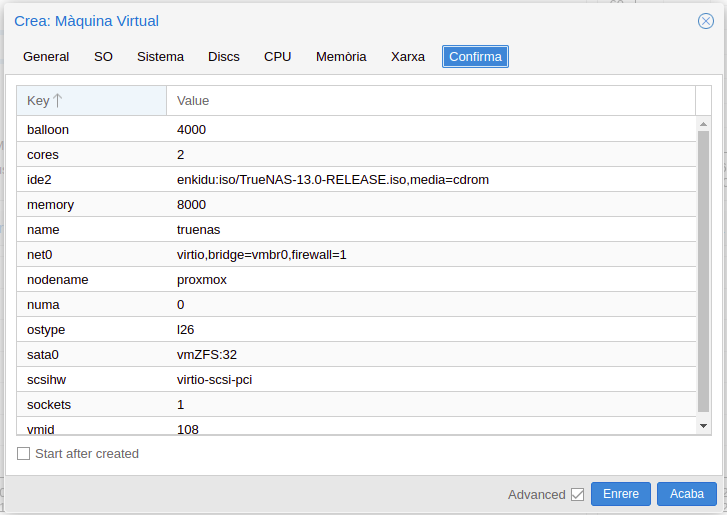
\includegraphics[width=0.5\textwidth,height=\textheight]{imatges/proxmox/install_truenas8.png}
\caption{Nova VM truenas}
\end{figure}

\hypertarget{contenidors-lxc-en-proxmox}{%
\section{Contenidors LXC en Proxmox}\label{contenidors-lxc-en-proxmox}}

Els contenidors són una alternativa lleugera a les màquines totalment virtualitzades (VM). Utilitzen el nucli del sistema amfitrió en què s'executen, en lloc d'emular un sistema operatiu (SO) complet.

Els costos d'execució dels contenidors són baixos, normalment insignificants. Tanmateix, hi ha alguns inconvenients que cal tenir en compte:

\begin{itemize}
\tightlist
\item
  Només es poden executar distribucions de Linux als contenidors Proxmox.
\item
  Per motius de seguretat, s'ha de restringir l'accés als recursos de l'amfitrió. Per tant, els contenidors s'executen en els seus propis espais de noms separats.
\end{itemize}

Proxmox VE fa servir \href{https://linuxcontainers.org/lxc/introduction/}{Linux Containers (LXC)} com a tecnologia de contenidors subjacent. Es gestiona amb ``Proxmox Container Toolkit'' ( pct ). Els contenidors estan estretament integrats amb Proxmox VE, podem utilitzar la mateixa xarxa i recursos d'emmagatzematge que les màquines virtuals.

\begin{rmdtip}{Tip}
Si voleu executar contenidors d'aplicacions, per exemple, imatges Docker, es recomana que els executeu dins d'una VM Proxmox Qemu.

\end{rmdtip}

\hypertarget{distribucions-suportades}{%
\subsection{Distribucions suportades}\label{distribucions-suportades}}

Basicament les més importants, algunes d'elles són

\begin{itemize}
\tightlist
\item
  \href{https://alpinelinux.org}{Alpine Linux}
\item
  \href{https://archlinux.org/}{Arch Linux}
\item
  \href{https://centos.org}{CentOS}
\item
  \href{https://www.debian.org}{Debian}
\item
  \href{https://ubuntu.com/}{Ubuntu} \ldots{}
\end{itemize}

\hypertarget{imatges-de-contenidors}{%
\subsection{Imatges de contenidors}\label{imatges-de-contenidors}}

Les imatges de contenidors, ``templates'' són arxius tar que contenen tot per executar un contenidor. Proxmox VE proporciona una varietat de plantilles bàsiques per a les distribucions de Linux més comunes. Es poden descarregar mitjançant la GUI o la utilitat de línia d'ordres pveam, també es poden descarregar plantilles de contenidors \href{https://www.turnkeylinux.org/}{TurnKey Linux}.

\begin{Shaded}
\begin{Highlighting}[]
\ExtensionTok{root@proxmox:\textasciitilde{}\#}\NormalTok{ pveam update}
\ExtensionTok{update}\NormalTok{ successful}
\ExtensionTok{root@proxmox:\textasciitilde{}\#}\NormalTok{ pveam available}
\ExtensionTok{mail}\NormalTok{            proxmox{-}mailgateway{-}6.4{-}standard\_6.4{-}1\_amd64.tar.gz}
\ExtensionTok{mail}\NormalTok{            proxmox{-}mailgateway{-}7.0{-}standard\_7.0{-}1\_amd64.tar.gz}
\ExtensionTok{system}\NormalTok{          almalinux{-}8{-}default\_20210928\_amd64.tar.xz}
\ExtensionTok{system}\NormalTok{          alpine{-}3.12{-}default\_20200823\_amd64.tar.xz}
\ExtensionTok{system}\NormalTok{          alpine{-}3.13{-}default\_20210419\_amd64.tar.xz}
\ExtensionTok{system}\NormalTok{          alpine{-}3.14{-}default\_20210623\_amd64.tar.xz}
\ExtensionTok{system}\NormalTok{          alpine{-}3.15{-}default\_20211202\_amd64.tar.xz}
\ExtensionTok{system}\NormalTok{          archlinux{-}base\_20211202{-}1\_amd64.tar.zst}
\ExtensionTok{system}\NormalTok{          centos{-}7{-}default\_20190926\_amd64.tar.xz}
\ExtensionTok{system}\NormalTok{          centos{-}8{-}default\_20201210\_amd64.tar.xz}
\ExtensionTok{system}\NormalTok{          centos{-}8{-}stream{-}default\_20220327\_amd64.tar.xz}
\ExtensionTok{system}\NormalTok{          debian{-}10{-}standard\_10.7{-}1\_amd64.tar.gz}
\ExtensionTok{system}\NormalTok{          debian{-}11{-}standard\_11.3{-}1\_amd64.tar.zst}
\ExtensionTok{system}\NormalTok{          devuan{-}3.0{-}standard\_3.0\_amd64.tar.gz}
\ExtensionTok{system}\NormalTok{          devuan{-}4.0{-}standard\_4.0\_amd64.tar.gz}
\ExtensionTok{system}\NormalTok{          fedora{-}34{-}default\_20}
\ExtensionTok{...}
\end{Highlighting}
\end{Shaded}

Abans de poder usar aquesta plantilla, cal que la descarregueu a un dels volums emmagatzematges. En el nostre cas en el volum backup que es on guardem les iso, VM i ara les imatges dels contenidors. Baixarem una Bebian 11, on després farem servir par Zoneminder.

\begin{Shaded}
\begin{Highlighting}[]
\ExtensionTok{root@proxmox:\textasciitilde{}\#}\NormalTok{ pveam download backup debian{-}11{-}standard\_11.3{-}1\_amd64.tar.zst}
\ExtensionTok{downloading}\NormalTok{ http://download.proxmox.com/images/system}\DataTypeTok{\textbackslash{}}
\NormalTok{/debian{-}11{-}standard\_11.3{-}1\_amd64.tar.zst to}\DataTypeTok{\textbackslash{}}
\NormalTok{/mnt/pve/backup/template/cache/debian{-}11{-}standard\_11.3{-}1\_amd64.tar.zst}
\ExtensionTok{{-}{-}2022{-}05{-}29}\NormalTok{ 23:10:05{-}{-}  }
\ExtensionTok{http://download.proxmox.com/images/system/debian{-}11{-}standard\_11.3{-}1\_amd64.tar.zst}
\ExtensionTok{Resolving}\NormalTok{ download.proxmox.com}\DataTypeTok{\textbackslash{}}
\ErrorTok{(}\ExtensionTok{download.proxmox.com}\KeywordTok{)}\ExtensionTok{...}\NormalTok{ 51.91.38.34, 2607:5300:203:7dc2::162}
\ExtensionTok{Connecting}\NormalTok{ to download.proxmox.com }\ErrorTok{(}\ExtensionTok{download.proxmox.com}\KeywordTok{)|}\ExtensionTok{51.91.38.34}\KeywordTok{|}\ExtensionTok{:80...}
\ExtensionTok{connected.}
\ExtensionTok{HTTP}\NormalTok{ request sent, awaiting response... 200 OK}
\ExtensionTok{Length:}\NormalTok{ 123216040 }\ErrorTok{(}\ExtensionTok{118M}\KeywordTok{)} \ExtensionTok{[application/octet{-}stream]}
\ExtensionTok{Saving}\NormalTok{ to:}
\StringTok{\textquotesingle{}/mnt/pve/backup/template/cache/debian{-}11{-}standard\_11.3{-}1\_amd64.tar.zst.tmp.195914\textquotesingle{}}
     \ExtensionTok{0K}\NormalTok{ ........ ........ ........ ........ 27\%  800K 1m49s}
 \ExtensionTok{32768K}\NormalTok{ ........ ........ ........ ........ 54\%  709K 73s}
 \ExtensionTok{65536K}\NormalTok{ ........ ........ ........ ........ 81\%  517K 34s}
 \ExtensionTok{98304K}\NormalTok{ ........ ........ .....            100\%  765K=2m59s}
\ExtensionTok{2022{-}05{-}29}\NormalTok{ 23:13:05 }\ErrorTok{(}\ExtensionTok{671}\NormalTok{ KB/s}\KeywordTok{)} \ExtensionTok{{-}}
\StringTok{\textquotesingle{}/mnt/pve/backup/template/cache/debian{-}11{-}standard\_11.3{-}1\_amd64.tar.zst.tmp.195914\textquotesingle{}}
\ExtensionTok{saved}\NormalTok{ [123216040/123216040]}

\ExtensionTok{calculating}\NormalTok{ checksum...OK, checksum verified}
\ExtensionTok{download}\NormalTok{ of}
\StringTok{\textquotesingle{}http://download.proxmox.com/images/system/debian{-}11{-}standard\_11.3{-}1\_amd64.tar.zst\textquotesingle{}}
\ExtensionTok{to} 
\StringTok{\textquotesingle{}/mnt/pve/backup/template/cache/debian{-}11{-}standard\_11.3{-}1\_amd64.tar.zst\textquotesingle{}}\NormalTok{ finished}
\end{Highlighting}
\end{Shaded}

Una vegada ja la tenim, procedirem a fer la instal·lacio d'un contenidor amb aquesta plantilla. Que utilitzarem per al servei de captura de video.

\hypertarget{creem-una-ct-amb-la-imatge-que-acabem-de-baixar}{%
\subsection{Creem una CT amb la imatge que acabem de baixar}\label{creem-una-ct-amb-la-imatge-que-acabem-de-baixar}}

\begin{figure}
\centering
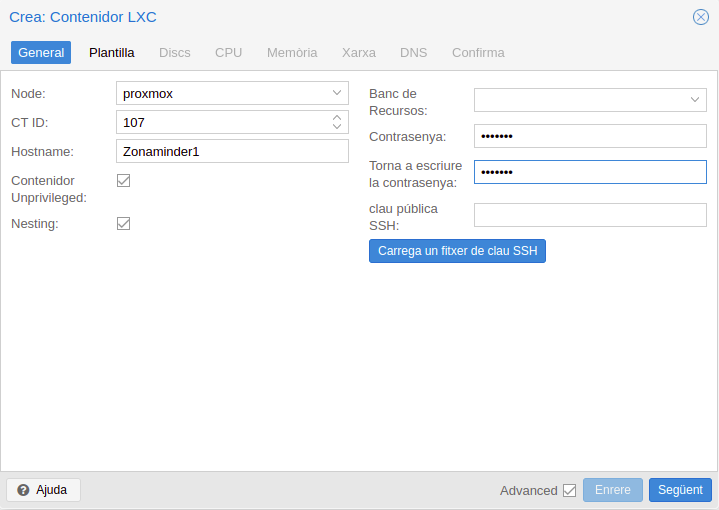
\includegraphics[width=0.5\textwidth,height=\textheight]{imatges/proxmox/Contenidor1.png}
\caption{Afegir contenidor}
\end{figure}

És molt paregut a la creacio de VM, pero en aquest cas hem de donar un password per al root del contenidor, i tindre en compte de marcar contenidor unprivileged.

\begin{rmdcuidao}{Ves amb compte}
Contenidors sense privilegis Els contenidors sense privilegis fan servir una nova característica del nucli anomenada espais de noms d'usuari. L'UID arrel 0 dins del contenidor està assignat a un usuari sense privilegis fora del contenidor. Això vol dir que la majoria dels problemes de seguretat (escapada de contenidors, ús abusiu de recursos, etc.) en aquests contenidors afectaran un usuari aleatori sense privilegis, i seria un error de seguretat genèric del nucli més que un problema de LXC. L'equip de LXC creu que els contenidors no privilegiats són segurs per disseny.

\end{rmdcuidao}

\begin{rmdtip}{Tip}
En l'apartat de disks, podem afegir nous discs i seleccionant el punt on es munta en mount points, en l'exemple en /mnt/espai. Es pot fer servir despres per muntar el volum de video de truenas, o fer-ho per NFS.

\end{rmdtip}

\begin{figure}
\centering
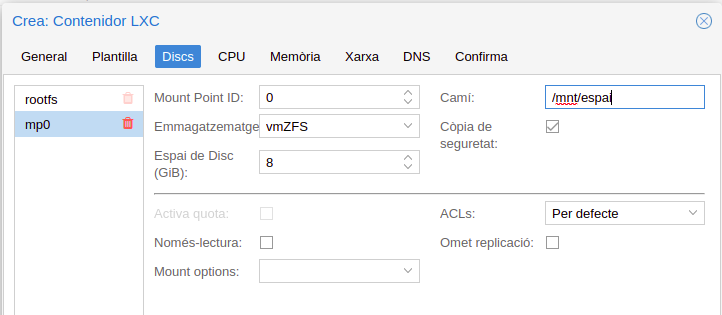
\includegraphics[width=0.5\textwidth,height=\textheight]{imatges/proxmox/mntEspai.png}
\caption{Punt de muntage}
\end{figure}

Punts de muntatge amb suport d'emmagatzematge Els punts de muntatge amb suport d'emmagatzematge els gestiona el subsistema d'emmagatzematge Proxmox VE i es presenten en tres tipus diferents:

\begin{itemize}
\item
  Basades en imatges: són imatges en brut que contenen un únic sistema de fitxers amb format ext4.
\item
  Subvolums ZFS: tècnicament són muntatges d'enllaç, però amb emmagatzematge gestionat i, per tant, permeten redimensionar i capturar instantànies.
\item
  Directoris: passar size=0 activa un cas especial en què es crea un directori en lloc d'una imatge en brut.
\end{itemize}

Per poder gestionar-lo en shell, camand pct

\begin{Shaded}
\begin{Highlighting}[]
\ExtensionTok{pct}\NormalTok{ start 100  }\CommentTok{\# arrancar}
\ExtensionTok{pct}\NormalTok{ console 100 }\CommentTok{\# inici de sessio}
\ExtensionTok{pct}\NormalTok{ enter 100 }\CommentTok{\# Shell amb root}
\ExtensionTok{...}
\end{Highlighting}
\end{Shaded}

Tambe el podem arrancar per la GUI, com cualsevol altra VM

\begin{figure}
\centering
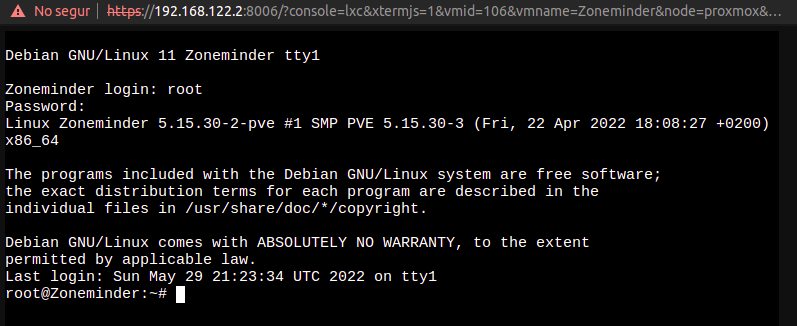
\includegraphics[width=0.8\textwidth,height=\textheight]{imatges/proxmox/contenedor_gui.png}
\caption{Contenedor amb la GUI}
\end{figure}

El primer que hem de fer es un upgrede i update. I ja està a punt per a gastar. Provem si té IP asignada.

\begin{Shaded}
\begin{Highlighting}[]
\ExtensionTok{root@Zoneminder:\textasciitilde{}\#}\NormalTok{ ip a}
\ExtensionTok{1:}\NormalTok{ lo: }\OperatorTok{\textless{}}\NormalTok{LOOPBACK,UP,LOWER\_UP}\OperatorTok{\textgreater{}}\NormalTok{ mtu 65536 qdisc noqueue state UNKNOWN}
\ExtensionTok{group}\NormalTok{ default qlen 1000}
    \ExtensionTok{link/loopback}\NormalTok{ 00:00:00:00:00:00 brd 00:00:00:00:00:00}
    \ExtensionTok{inet}\NormalTok{ 127.0.0.1/8 scope host lo}
       \ExtensionTok{valid\_lft}\NormalTok{ forever preferred\_lft forever}
    \ExtensionTok{inet6}\NormalTok{ ::1/128 scope host }
       \ExtensionTok{valid\_lft}\NormalTok{ forever preferred\_lft forever}
\ExtensionTok{2:}\NormalTok{ eth0@if33: }\OperatorTok{\textless{}}\NormalTok{BROADCAST,MULTICAST,UP,LOWER\_UP}\OperatorTok{\textgreater{}}\NormalTok{ mtu 1500 qdisc noqueue}
\ExtensionTok{state}\NormalTok{ UP group default qlen 1000}
    \ExtensionTok{link/ether}\NormalTok{ 9e:ab:81:76:34:b7 brd ff:ff:ff:ff:ff:ff link{-}netnsid 0}
    \ExtensionTok{inet}\NormalTok{ 192.168.122.250/24 brd 192.168.122.255 scope global dynamic eth0}
       \ExtensionTok{valid\_lft}\NormalTok{ 3416sec preferred\_lft 3416sec}
    \ExtensionTok{inet6}\NormalTok{ fe80::9cab:81ff:fe76:34b7/64 scope link }
       \ExtensionTok{valid\_lft}\NormalTok{ forever preferred\_lft forever}
\ExtensionTok{root@Zoneminder:\textasciitilde{}\#} 
\end{Highlighting}
\end{Shaded}

\hypertarget{subxarxes-en-proxmox}{%
\section{Subxarxes en Proxmox}\label{subxarxes-en-proxmox}}

\href{https://pve.proxmox.com/wiki/Open_vSwitch}{Documentacio oficial} \href{https://www.openvswitch.org/}{Open vswitch} \href{https://webworxshop.com/virtualised-pfsense-on-proxmox-with-open-vswitch/}{PfSense virtualitzat a Proxmox amb Open vSwitch}

Crearem la xarxa interna per a les VM la forma mes facil és per \href{https://www.openvswitch.org/}{Open vSwitch}, té una lògica més neta que el pont Linux i està dissenyat específicament per funcionar en entorns virtualitzats.

En la consola de Proxmox instal·lem openvswitch-switch, no s'instal·la de manera predeterminada.

\begin{Shaded}
\begin{Highlighting}[]
\ExtensionTok{apt}\NormalTok{ update}
\ExtensionTok{apt}\NormalTok{ install openvswitch{-}switch}
\end{Highlighting}
\end{Shaded}

\begin{rmdwarn}{Perill}
Es recomana que el pont estiga lligat a un port troncal sense vlans sense etiquetar; això vol dir que el nostre pont mai tindrà una adreça IP. Dividim les nostres VLAN etiquetades mitjançant interfícies virtuals (OVSIntPort) per si necessitem accedir a aquestes VLAN des de la nostra host local. Proxmox assignarà a les màquines virtuals convidades una interfície de toc associada a una vlan, de manera que no necessitem un pont per vlan

\end{rmdwarn}

Per dividir les vlans amb ips per utilitzar-les a l'amfitrió local, hauríem d'utilitzar OVSIntPorts

Perquè l'amfitrió (per exemple, l'amfitrió proxmox, no les màquines virtuals, utilitze una vlan dins del pont, heu de crear OVSIntPorts. Per a VLAN 1 que dona flux d'espai d'emmagatzenament.)

\begin{rmdcuidao}{OVSintPorts}
Aquests OVSintPorts que creeu també han d'aparéixer a la definició del pont real a ovs\_ports. Si no ho fan, no es mostraran encara que hàgeu especificat un ovs\_bridge.

\end{rmdcuidao}

La diferència principal és que en lloc de tidre un pont per vlan, tenim un únic pont que conté totes les nostres vlan. Aleshores, quan configureu la interfície de xarxa per a la màquina virtual, seleccionareu el pont nou pont OVS i li assignem una VLAN.

Quedaria

\begin{figure}
\centering
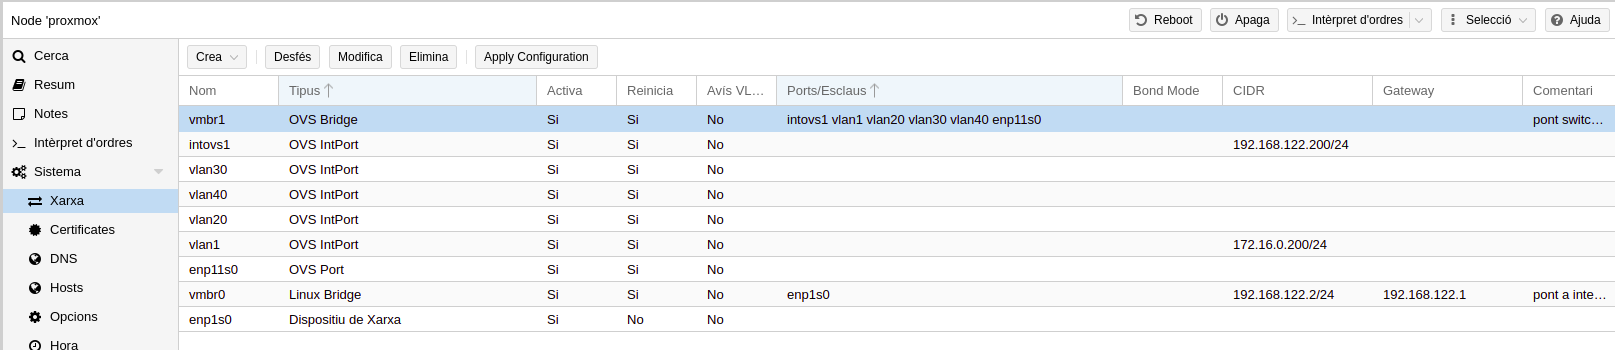
\includegraphics[width=0.8\textwidth,height=\textheight]{imatges/proxmox/xarxa_ovs.png}
\caption{xarxa OVS}
\end{figure}

El pont vmbr0 és un pont linux, és el que es crea automaticament en instal·lar Proxmox. Que està connectat a enp1s0, que és la interfase que ell creu real del servidor (dispositiu de xarxa). Aquest pont té la IP 192.168.122.2/24 i gateway 192.168.122.1 és per on entra internet NAT des de la host. No és convenient tindre xarxes linux i xarxer OVS barretjades. Hauriem d'eliminar aquest pont i connectar le enp1s0 al nou pont OVS vmbr1 directament, de moment he preferit no tocar res, ja que molts problemes que he tingut en les xarxes és per la configuracio de la prova. Virtualitzar el proxmox. En el cas real, o en la seguent fase de les proves, el Proxmox anira directament al hardware de la màquina, sense ser virtualitzat. Com de moment funciona, no fare més proves per aquest cami, que no adelenta res en el resultat final.

El vmbr1 es el pont OVS que hem creat per a la xarxa interna de les VM, es tan sencill com anar a xarxes i crea nou pont OVS

\begin{figure}
\centering
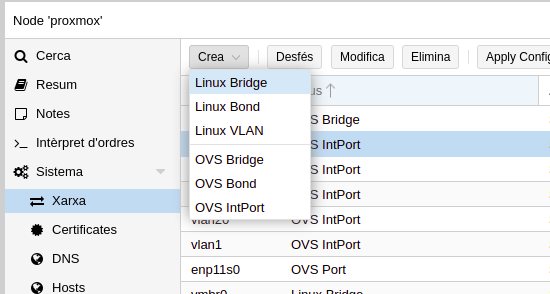
\includegraphics[width=0.5\textwidth,height=\textheight]{imatges/proxmox/Pont_OVS1.png}
\caption{Pont OVS}
\end{figure}

En aquest pont OVS, no li donem IP ni gateway (pren la predeterminada del sistema, la definida en vmBr0). En font li diguem les interfices que estan connectades, la intovs1 (és la interfase internade proxmox que es connecta a la xarxa NAT), i les VLAN 1 20 30 40 que són les interfases internas de proxmox per a les VLAN que crearem a continuacio. Són per a què Proxmox és conecta a aquestes VLAN, la veritat és que soles ens faria falta la VLAN 1 que és per on comparteix l'espai de backup truenas.

\begin{figure}
\centering
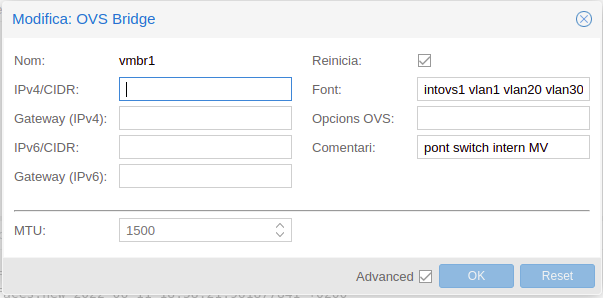
\includegraphics[width=0.5\textwidth,height=\textheight]{imatges/proxmox/pont_OVS2.png}
\caption{Pont OVS}
\end{figure}

\begin{rmdtip}{Tip}
En el cas posterio que eliminem el pont vmbr0, si li tindriem que donar la IP i el gateway, com els que te aquest.

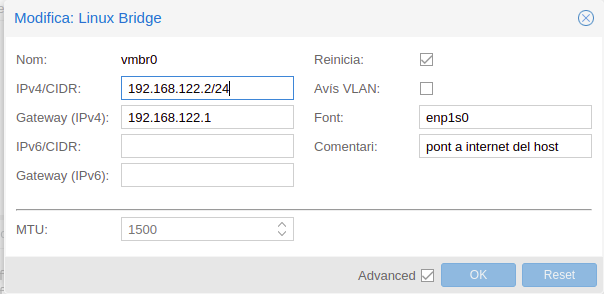
\includegraphics[width=0.5\textwidth,height=\textheight]{imatges/proxmox/vmBr0.png}

\end{rmdtip}

Per crear una OVS intport, igual que hem fet en el pont pero ara elegim intPort

\begin{enumerate}
\def\labelenumi{\arabic{enumi}.}
\tightlist
\item
  Li donem un nom, li he posat VLAN 1, haguera sigut millor dir-li TeagetaVlan1
\item
  Li donem IP estatica
\item
  La vinculem al pont OVS vmbr1
\end{enumerate}

\begin{figure}
\centering
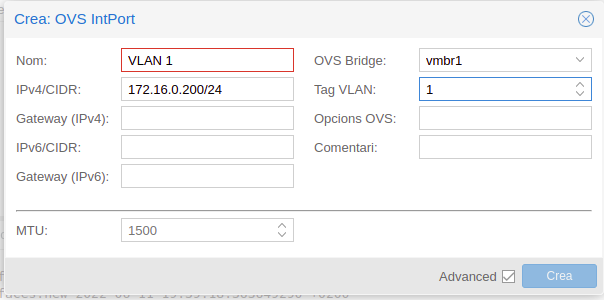
\includegraphics[width=0.5\textwidth,height=\textheight]{imatges/proxmox/Intport_VLAN1.png}
\caption{IntPort per a VLAN 1 de proxmox}
\end{figure}

Quedaria per a cada VM maquinari -\textgreater{} afegir -\textgreater{} dispositiu de xarxa, crear una interfase de xarxa nova, asociarla al pont OVS i seleccionar la VLAN a la qual es connecta.

\begin{figure}
\centering
\includegraphics[width=0.5\textwidth,height=\textheight]{imatges/proxmox/truenas_xarxa3.png}
\caption{Xarxa Truenas}
\end{figure}

\begin{figure}
\centering
\includegraphics[width=0.5\textwidth,height=\textheight]{imatges/proxmox/interface_vlan.png}
\caption{nova interfase}
\end{figure}

Veiem que tenim net1 al pont vmbr0, està l'eliminariem, una vegada tot configurat, és la que he utilitzat per fer les configuracions des del navegadordel host local per comoditat.

En el cas de pfSense, no li afegim una targeta de xarxa per a cada VLAN. Li afegim soles una sense definir la VLAN, i OVS la tacta com a Trunk, per on van totes les xarxes. Des de dins de pfSense, es creen les diferents interfases per a cada VLAN.

Fem un ping a la IP de pfSense en la VLAN 1 des de Proxmox per comprovar que esten en la VLAN 1

\begin{Shaded}
\begin{Highlighting}[]
\ExtensionTok{root@proxmox:\textasciitilde{}\#}\NormalTok{ ping 172.16.0.254}
\ExtensionTok{PING}\NormalTok{ 172.16.0.254 }\ErrorTok{(}\ExtensionTok{172.16.0.254}\KeywordTok{)} \ExtensionTok{56}\ErrorTok{(}\ExtensionTok{84}\KeywordTok{)} \ExtensionTok{bytes}\NormalTok{ of data.}
\ExtensionTok{64}\NormalTok{ bytes from 172.16.0.254: icmp\_seq=1 ttl=64 time=5.79 ms}
\ExtensionTok{64}\NormalTok{ bytes from 172.16.0.254: icmp\_seq=2 ttl=64 time=2.70 ms}

\ExtensionTok{{-}{-}{-}}\NormalTok{ 172.16.0.254 ping statistics }\AttributeTok{{-}{-}{-}}
\ExtensionTok{2}\NormalTok{ packets transmitted, 2 received, 0\% packet loss, time 1002ms}
\ExtensionTok{rtt}\NormalTok{ min/avg/max/mdev = 2.698/4.245/5.792/1.547 ms}
\end{Highlighting}
\end{Shaded}

\hypertarget{segon-intercace-post-install}{%
\subsection{Segon intercace, post install}\label{segon-intercace-post-install}}

En el cas real, o en la seguent fase de les proves aquest apartat no és necesari, és soles per poder traure la xarxa interna a l'exterior, queda per acabar de configurar.

La primera la crea automàticament i la tenim en NAT, es la que anirà connectada directament l'encaminador que ens dona internet.

Farem un pont en el host per simular l'altra interfices del servidor, una anirà pel primer pont en NAT, i l'altra la connectem a enp3s0 que és l'ethernet física del portàtil, per connectar aquesta a un encaminador casolà que farà de switch, o el switch físic real.

\href{https://linuxconfig.org/how-to-use-bridged-networking-with-libvirt-and-kvm}{Documentacio pont linux}

El dimoni libvirtd s'està executant, es crea una xarxa per defecte. Podem comprovar que aquesta xarxa existeix mitjançant la virsh

\begin{Shaded}
\begin{Highlighting}[]
\ExtensionTok{$}\NormalTok{ sudo virsh net{-}list }\AttributeTok{{-}{-}all}
 \ExtensionTok{Name}\NormalTok{      State    Autostart   Persistent}
\ExtensionTok{{-}{-}{-}{-}{-}{-}{-}{-}{-}{-}{-}{-}{-}{-}{-}{-}{-}{-}{-}{-}{-}{-}{-}{-}{-}{-}{-}{-}{-}{-}{-}{-}{-}{-}{-}{-}{-}{-}{-}{-}{-}{-}{-}{-}}
 \ExtensionTok{default}\NormalTok{   active   yes         yes}
\end{Highlighting}
\end{Shaded}

La seua configuració es

\begin{Shaded}
\begin{Highlighting}[]
\FunctionTok{sudo}\NormalTok{ virsh net{-}edit default}
\end{Highlighting}
\end{Shaded}

\begin{Shaded}
\begin{Highlighting}[]
\NormalTok{\textless{}}\KeywordTok{network}\NormalTok{\textgreater{}}
\NormalTok{  \textless{}}\KeywordTok{name}\NormalTok{\textgreater{}default\textless{}/}\KeywordTok{name}\NormalTok{\textgreater{}}
\NormalTok{  \textless{}}\KeywordTok{uuid}\NormalTok{\textgreater{}4aee1ff6{-}80c4{-}4edb{-}b155{-}7abd67ca293a\textless{}/}\KeywordTok{uuid}\NormalTok{\textgreater{}}
\NormalTok{  \textless{}}\KeywordTok{forward}\OtherTok{ mode=}\StringTok{\textquotesingle{}nat\textquotesingle{}}\NormalTok{/\textgreater{}}
\NormalTok{  \textless{}}\KeywordTok{bridge}\OtherTok{ name=}\StringTok{\textquotesingle{}virbr0\textquotesingle{}}\OtherTok{ stp=}\StringTok{\textquotesingle{}on\textquotesingle{}}\OtherTok{ delay=}\StringTok{\textquotesingle{}0\textquotesingle{}}\NormalTok{/\textgreater{}}
\NormalTok{  \textless{}}\KeywordTok{mac}\OtherTok{ address=}\StringTok{\textquotesingle{}52:54:00:d5:0b:34\textquotesingle{}}\NormalTok{/\textgreater{}}
\NormalTok{  \textless{}}\KeywordTok{ip}\OtherTok{ address=}\StringTok{\textquotesingle{}192.168.122.1\textquotesingle{}}\OtherTok{ netmask=}\StringTok{\textquotesingle{}255.255.255.0\textquotesingle{}}\NormalTok{\textgreater{}}
\NormalTok{    \textless{}}\KeywordTok{dhcp}\NormalTok{\textgreater{}}
\NormalTok{      \textless{}}\KeywordTok{range}\OtherTok{ start=}\StringTok{\textquotesingle{}192.168.122.2\textquotesingle{}}\OtherTok{ end=}\StringTok{\textquotesingle{}192.168.122.254\textquotesingle{}}\NormalTok{/\textgreater{}}
\NormalTok{    \textless{}/}\KeywordTok{dhcp}\NormalTok{\textgreater{}}
\NormalTok{  \textless{}/}\KeywordTok{ip}\NormalTok{\textgreater{}}
\NormalTok{\textless{}/}\KeywordTok{network}\NormalTok{\textgreater{}}
\end{Highlighting}
\end{Shaded}

virbr0 utilitza connectivitat basada en NAT per connectar les màquines virtuals que formen part de la xarxa amb el món exterior. Tenint activat servei DHCP.

Per veure qui esta connectat aquest pont

\begin{Shaded}
\begin{Highlighting}[]
\ExtensionTok{$}\NormalTok{ ip link show master virbr0  }
\ExtensionTok{16:}\NormalTok{ vnet5: }\OperatorTok{\textless{}}\NormalTok{BROADCAST,MULTICAST,UP,LOWER\_UP}\OperatorTok{\textgreater{}}\NormalTok{ mtu 1500 qdisc }
\ExtensionTok{noqueue}\NormalTok{ master virbr0 state UNKNOWN mode DEFAULT group default qlen 1000}
    \ExtensionTok{link/ether}\NormalTok{ fe:54:00:df:dd:09 brd ff:ff:ff:ff:ff:ff}
\end{Highlighting}
\end{Shaded}

Soles tenim connectada la vnet5, que apareix en arrancar la màquina virtual,

El que volem es una connexió de pont completa, on els dispositius convidats estan connectats a la LAN amfitrió, sense fer servir NAT, hauríem de crear un nou pont i compartir una de les interfícies físiques d'Ethernet de l'amfitrió.

Primer creem un nou pont anomenat br0 i mostrem els ports

\begin{Shaded}
\begin{Highlighting}[]
\ExtensionTok{$}\NormalTok{ sudo ip link add br0 type bridge}
\ExtensionTok{$}\NormalTok{ sudo ip link show type bridge}
\ExtensionTok{8:}\NormalTok{ virbr0: }\OperatorTok{\textless{}}\NormalTok{BROADCAST,MULTICAST,UP,LOWER\_UP}\OperatorTok{\textgreater{}}\NormalTok{ mtu 1500 qdisc noqueue }
\ExtensionTok{state}\NormalTok{ UP mode DEFAULT group default qlen 1000}
    \ExtensionTok{link/ether}\NormalTok{ 52:54:00:d5:0b:34 brd ff:ff:ff:ff:ff:ff}
\ExtensionTok{17:}\NormalTok{ br0: }\OperatorTok{\textless{}}\NormalTok{BROADCAST,MULTICAST}\OperatorTok{\textgreater{}}\NormalTok{ mtu 1500 qdisc noop}
\ExtensionTok{state}\NormalTok{ DOWN mode DEFAULT group default qlen 1000}
    \ExtensionTok{link/ether}\NormalTok{ 82:bd:1e:40:5c:fd brd ff:ff:ff:ff:ff:ff}
\end{Highlighting}
\end{Shaded}

Li afegirem la interfície física host enp3s0, faig servir la de xarxa, perquè per a la connectivitat faig gastar la wifi, si connectàrem aquesta, perdríem la connectivitat, ja que perdria la seua IP.

Primer l'alcem i l'afegim al pont

\begin{Shaded}
\begin{Highlighting}[]
\ExtensionTok{$}\NormalTok{ sudo ip link set enp3s0 up}
\ExtensionTok{$}\NormalTok{ sudo ip link set enp3s0 master br0}

\ExtensionTok{RTNETLINK}\NormalTok{ answers: Operation not supported}
\end{Highlighting}
\end{Shaded}

De moment no va, queda pendent resoldre-ho, provarem una altra via, macvtap

\href{https://blog.scottlowe.org/2016/02/09/using-kvm-libvirt-macvtap-interfaces/}{macvtap} és per connectar interfícies de contenidors directament amb interfícies d'amfitrió.

Provar que ho soporta el nucli

\begin{Shaded}
\begin{Highlighting}[]
\ExtensionTok{$}\NormalTok{ sudo modprobe macvlan}
\FunctionTok{lsmod} \KeywordTok{|} \FunctionTok{grep}\NormalTok{ macvlan}
\end{Highlighting}
\end{Shaded}

Fer el fitxer xml on definim el pont macvtap

\begin{Shaded}
\begin{Highlighting}[]
\NormalTok{\textless{}}\KeywordTok{network}\NormalTok{\textgreater{}}
\NormalTok{  \textless{}}\KeywordTok{name}\NormalTok{\textgreater{}macvtap{-}net\textless{}/}\KeywordTok{name}\NormalTok{\textgreater{}}
\NormalTok{  \textless{}}\KeywordTok{forward}\OtherTok{ mode=}\StringTok{"bridge"}\NormalTok{\textgreater{}}
\NormalTok{    \textless{}}\KeywordTok{interface}\OtherTok{ dev=}\StringTok{"enp3s0"}\NormalTok{/\textgreater{}}
\NormalTok{  \textless{}/}\KeywordTok{forward}\NormalTok{\textgreater{}}
\NormalTok{\textless{}/}\KeywordTok{network}\NormalTok{\textgreater{}}
\end{Highlighting}
\end{Shaded}

Per enllaçar directament a enp3s0 Feu servir l'virsh net-defineordre amb aquest XML per definir la xarxa Libvirt real. El fitxer anterior està en macvtap\_enp3s0.xml

\begin{Shaded}
\begin{Highlighting}[]
\ExtensionTok{virsh}\NormalTok{ net{-}define macvtap\_enp3s0.xml}
\ExtensionTok{Network}\NormalTok{ macvtap{-}net defined from macvtap\_enp3s0.xml}
\end{Highlighting}
\end{Shaded}

A continuació, establiríem la xarxa Libvirt resultant per iniciar-la automàticament.

\begin{Shaded}
\begin{Highlighting}[]
\ExtensionTok{$}\NormalTok{ sudo virsh net{-}autostart macvtap{-}net}
\ExtensionTok{Network}\NormalTok{ macvtap{-}net marked as autostarted}
\ExtensionTok{$}\NormalTok{ sudo virsh net{-}start macvtap{-}net}
\ExtensionTok{Network}\NormalTok{ macvtap{-}net started}
\end{Highlighting}
\end{Shaded}

Després la connectem a la VM proxmox

\begin{figure}
\centering
\includegraphics[width=0.5\textwidth,height=\textheight]{imatges/proxmox/macvtap.png}
\caption{segon interficei connectada directa a enp3s0}
\end{figure}

Aquest mètode si funciona, ja tenim les dues xarxes al servidor, ara hem de configurar el pfsense perquè es connecte al switch per aquesta i podríem connectar als recursos del servidor des d'un altre ordinador concertat a un router.

\hypertarget{cuxf2pies-de-seguretat}{%
\section{Còpies de seguretat}\label{cuxf2pies-de-seguretat}}

Les imatges de les VM no haurien de canviar molt en el temps, per això, tindrem una politica de còpies de seguretat d'una vegada al mes, mantenint la primera configuracio blocada a l'esborrat.

Durem a terme aquesta tasca amb l'opcio que de backup que porta el GUI, tenint en compte de no afegir discs durs secondaris de les VM si en tingueren, no es el cas, en la forma que ho hem configurat, l'espai per a dades el compartim per xarxa, i no entra en le backup per defecte.

Per fer les còpies de seguretat de les VM anem a centre de dades En centre de dades -\textgreater{} còpia de seguretat -\textgreater{} afegir nova ens ix el seguent panell.

\begin{enumerate}
\def\labelenumi{\arabic{enumi}.}
\tightlist
\item
  Node, el nostre node, soles en tenim un.
\item
  Emmagatzenament, on volem que es cree la imatge, en Backup que es l'espai compartit pel nas.
\item
  Programes, configurem la frecuancia de les còpies, una al mes a les 3 a.m.
\item
  Elmode, soles les escollides, ja que la de Truenas no volem que la faça.
\item
  Compresio, podem elegir el tipus, que compremeix mes i tarda més, el de per defecte va bé.
\item
  El mode, seleccionem si volem instantanea, suspensio o aturada, le més segura és aturada, i com les farem a altes hores i no tindra usuaris el servei, no deu ser problema, si no podera para, es faria instanatanea.
\end{enumerate}

\begin{figure}
\centering
\includegraphics[width=0.5\textwidth,height=\textheight]{imatges/proxmox/backup1.png}
\caption{Configurar la còpia de seguretat de les VM}
\end{figure}

En l'opcio retention configurem perquè soles guarde les dues últimes.

\begin{figure}
\centering
\includegraphics[width=0.5\textwidth,height=\textheight]{imatges/proxmox/backup2.png}
\caption{Seleccionar les remanents}
\end{figure}

Per conservar una imatge determinada, en el nostre cas la primera de configuracio inicial, en el volum on estan guardades, backup, seleccionem la que volem protegir i li canviem en change protection que deuria d'apareixer ara l'escut.

\begin{figure}
\centering
\includegraphics[width=0.8\textwidth,height=\textheight]{imatges/proxmox/protect.png}
\caption{Ramanencia d'una còpia en concret}
\end{figure}

\hypertarget{copia-de-seguretat-de-truena}{%
\subsection{Copia de seguretat de truena}\label{copia-de-seguretat-de-truena}}

No podem fer una còpia de seguretat de Truenas i guardar-la per xarxa en Truenas. En principi es podria fer una instanatanea, pero s'atura el servei i es queda clavat.

Farem còpia de seguretat en local i després la pasarem al directori de Backup amb rsync. La fem com en el cas anterior, pero ara la guardarem en local.

\begin{figure}
\centering
\includegraphics[width=0.5\textwidth,height=\textheight]{imatges/proxmox/copia_seguretat_Truenas_local.png}
\caption{Còpia de seguretat Truenas local}
\end{figure}

i li diguem que guarde les dues últimes

Les guada en \emph{./var/lib/vz/dump/vzdump-qemu-102-2022\_05\_27-22\_27\_02.vma.zst} les passarem per rsync al directori de backup de les VM compartit per Tuenas, està en \emph{/mnt/pve/backup/dump}

\begin{Shaded}
\begin{Highlighting}[]
\ExtensionTok{root@proxmox:/mnt/pve/backup/dump\#}\NormalTok{ ls}
\ExtensionTok{vzdump{-}qemu{-}105{-}2022\_06\_02{-}00\_02\_12.log}
\ExtensionTok{vzdump{-}qemu{-}107{-}2022\_05\_30{-}23\_54\_17.log}
\ExtensionTok{vzdump{-}qemu{-}105{-}2022\_06\_02{-}00\_02\_12.vma.zst}
\ExtensionTok{vzdump{-}qemu{-}107{-}2022\_05\_30{-}23\_54\_17.vma.zst}
\ExtensionTok{vzdump{-}qemu{-}105{-}2022\_06\_02{-}00\_02\_12.vma.zst.notes}
\ExtensionTok{vzdump{-}qemu{-}107{-}2022\_05\_30{-}23\_54\_17.vma.zst.notes}
\ExtensionTok{vzdump{-}qemu{-}107{-}2022\_05\_30{-}23\_49\_20.log}
\ExtensionTok{root@proxmox:/mnt/pve/backup/dump\#}\NormalTok{ rsync }\AttributeTok{{-}a}\NormalTok{ /var/lib/vz/dump/ /mnt/pve/backup/dump}
\end{Highlighting}
\end{Shaded}

Quan acaba, ja ens apareix en l'espai d'emmagatzenamet backup.

\begin{figure}
\centering
\includegraphics[width=0.8\textwidth,height=\textheight]{imatges/proxmox/rsync_tue.png}
\caption{Sincronitzacio de la imatge Truanas}
\end{figure}

Farem un scipt perquè sincronitze el directori local amb del backup i ho afegirem a cron en la periocitat bque hem definit per a fer les còpies, en principi a principi de cada mes, deixarem un marge de temps i sincronitzarem una hora després.

\begin{Shaded}
\begin{Highlighting}[]
\CommentTok{\#!/bin/sh}
\FunctionTok{rsync} \AttributeTok{{-}a}\NormalTok{ /var/lib/vz/dump/ /mnt/pve/backup/dump}
\end{Highlighting}
\end{Shaded}

\hypertarget{cuxf2pia-de-seguretat-de-proxmox}{%
\subsection{Còpia de seguretat de Proxmox}\label{cuxf2pia-de-seguretat-de-proxmox}}

Com el sistema base de proxmox, una Debian 11 està en un volum ZFS fem un clon de rpool que es un estan el directori arrel i el guardem en l'espai Backup en el servidor nas.

\begin{rmdwarn}{Perill}
Com estem en el porces de proves i no voldria trencar les cosesque de moment van, he efegit un altre disc virtual la VM de proxmox l'hem creat un colum ZFS que es diu vmZFS1 per fer les proves de clonacio. en backup seria igual pero encaminant al directori on està muntat vmZFS

\end{rmdwarn}

Primer mirem els pools que té proxmox

\begin{Shaded}
\begin{Highlighting}[]
\ExtensionTok{root@proxmox:\textasciitilde{}\#}\NormalTok{ zpool status}
  \ExtensionTok{pool:}\NormalTok{ rpool}
 \ExtensionTok{state:}\NormalTok{ ONLINE}
\ExtensionTok{config:}

        \ExtensionTok{NAME}\NormalTok{        STATE     READ WRITE CKSUM}
        \ExtensionTok{rpool}\NormalTok{       ONLINE       0     0     0}
          \ExtensionTok{vda3}\NormalTok{      ONLINE       0     0     0}

\ExtensionTok{errors:}\NormalTok{ No known data errors}

  \ExtensionTok{pool:}\NormalTok{ vmZFS}
 \ExtensionTok{state:}\NormalTok{ ONLINE}
\ExtensionTok{config:}

        \ExtensionTok{NAME}\NormalTok{        STATE     READ WRITE CKSUM}
        \ExtensionTok{vmZFS}\NormalTok{       ONLINE       0     0     0}
          \ExtensionTok{vdb}\NormalTok{       ONLINE       0     0     0}

\ExtensionTok{errors:}\NormalTok{ No known data errors}

  \ExtensionTok{pool:}\NormalTok{ vmZFS1}
 \ExtensionTok{state:}\NormalTok{ ONLINE}
\ExtensionTok{config:}

        \ExtensionTok{NAME}\NormalTok{        STATE     READ WRITE CKSUM}
        \ExtensionTok{vmZFS1}\NormalTok{      ONLINE       0     0     0}
          \ExtensionTok{vde}\NormalTok{       ONLINE       0     0     0}

\ExtensionTok{errors:}\NormalTok{ No known data errors}

  \ExtensionTok{pool:}\NormalTok{ zfspool1}
 \ExtensionTok{state:}\NormalTok{ ONLINE}
\ExtensionTok{config:}

        \ExtensionTok{NAME}\NormalTok{        STATE     READ WRITE CKSUM}
        \ExtensionTok{zfspool1}\NormalTok{    ONLINE       0     0     0}
          \ExtensionTok{vdc}\NormalTok{       ONLINE       0     0     0}
          \ExtensionTok{vdd}\NormalTok{       ONLINE       0     0     0}

\ExtensionTok{errors:}\NormalTok{ No known data errors}
\ExtensionTok{root@proxmox:\textasciitilde{}\#}\NormalTok{ zfs list }\AttributeTok{{-}r}\NormalTok{ rpool}
\ExtensionTok{NAME}\NormalTok{               USED  AVAIL     REFER  MOUNTPOINT}
\ExtensionTok{rpool}\NormalTok{             15.2G  22.6G       96K  /rpool}
\ExtensionTok{rpool/ROOT}\NormalTok{        15.2G  22.6G       96K  /rpool/ROOT}
\ExtensionTok{rpool/ROOT/pve{-}1}\NormalTok{  15.2G  22.6G     15.2G  /}
\ExtensionTok{rpool/data}\NormalTok{         15}
\end{Highlighting}
\end{Shaded}

El sistema base Debian de proxmox està en rpool, i l'arrel en rpool/ROOT/pve-1. Per poder clonar, primer hem de fer un snapshot i després clonar d'aques snap segons la documentacio \href{https://www.howtoforge.com/tutorial/how-to-use-snapshots-clones-and-replication-in-zfs-on-linux/}{clones ZFS}

\begin{Shaded}
\begin{Highlighting}[]

\ExtensionTok{root@proxmox:/rpool\#}\NormalTok{ df}
\ExtensionTok{Filesystem}\NormalTok{                         1K{-}blocks     Used Available Use\% Mounted on}
\ExtensionTok{udev}\NormalTok{                                14001688        0  14001688   0\% /dev}
\ExtensionTok{tmpfs}\NormalTok{                                2807172     1304   2805868   1\% /run}
\ExtensionTok{rpool/ROOT/pve{-}1}\NormalTok{                    39619072 15897344  23721728  41\% /}
\ExtensionTok{tmpfs}\NormalTok{                               14035840    43680  13992160   1\% /dev/shm}
\ExtensionTok{tmpfs}\NormalTok{                                   5120        0      5120   0\% /run/lock}
\ExtensionTok{vmZFS}\NormalTok{                               68554496      128  68554368   1\% /vmZFS}
\ExtensionTok{rpool}\NormalTok{                               23721856      128  23721728   1\% /rpool}
\ExtensionTok{rpool/data}\NormalTok{                          23721856      128  23721728   1\% /rpool/data}
\ExtensionTok{rpool/ROOT}\NormalTok{                          23721856      128  23721728   1\% /rpool/ROOT}
\ExtensionTok{zfspool1}\NormalTok{                               13056      128     12928   1\% /mnt/zfspool1}
\ExtensionTok{/dev/fuse}\NormalTok{                             131072       20    131052   1\% /etc/pve}
\ExtensionTok{vmZFS1}\NormalTok{                             101088768      128 101088640   1\% /vmZFS1}
\ExtensionTok{172.16.0.4:/mnt/datatruenas/backup}\NormalTok{  55712384  5337856  50374528  10\% /mnt/pve/backup}
\ExtensionTok{vmZFS1/backup}\NormalTok{                      101088768      128 101088640   1\% /vmZFS1/backup}
\ExtensionTok{tmpfs}\NormalTok{                                2807168        0   2807168   0\% /run/user/0}
\ExtensionTok{root@proxmox:/rpool\#}\NormalTok{ zfs snapshot rpool/ROOT/pve{-}1@today}
\ExtensionTok{root@proxmox:/rpool\#}\NormalTok{ zfs list }\AttributeTok{{-}t}\NormalTok{ snapshot}
\ExtensionTok{NAME}\NormalTok{                             USED  AVAIL     REFER  MOUNTPOINT}
\ExtensionTok{rpool@proxmox}\NormalTok{                      0B      }\AttributeTok{{-}}\NormalTok{       96K  }\AttributeTok{{-}}
\ExtensionTok{rpool@today}\NormalTok{                        0B      }\AttributeTok{{-}}\NormalTok{       96K  }\AttributeTok{{-}}
\ExtensionTok{rpool/ROOT@base\_data}\NormalTok{              64K      }\AttributeTok{{-}}\NormalTok{       96K  }\AttributeTok{{-}}
\ExtensionTok{rpool/ROOT/pve{-}1@today}\NormalTok{          1.72M      }\AttributeTok{{-}}\NormalTok{     15.2G  }\AttributeTok{{-}}
\ExtensionTok{rpool/data@base\_data}\NormalTok{              56K      }\AttributeTok{{-}}\NormalTok{       96K  }\AttributeTok{{-}}
\ExtensionTok{vmZFS/base{-}103{-}disk{-}0@\_\_base\_\_}\NormalTok{     8K      }\AttributeTok{{-}}\NormalTok{     2.69G  }\AttributeTok{{-}}
\ExtensionTok{vmZFS/vm{-}100{-}disk{-}0@pfsense}\NormalTok{      310M      }\AttributeTok{{-}}\NormalTok{     1.24G  }\AttributeTok{{-}}
\ExtensionTok{vmZFS1/backup@today}\NormalTok{                0B      }\AttributeTok{{-}}\NormalTok{       96K  }\AttributeTok{{-}}
\ExtensionTok{root@proxmox:/rpool\#}\NormalTok{ zfs send rpool/ROOT/pve{-}1@today }\KeywordTok{|} \ExtensionTok{zfs}\NormalTok{ receive vmZFS1/backup}
\ExtensionTok{cannot}\NormalTok{ receive new filesystem stream: destination }\StringTok{\textquotesingle{}vmZFS1/backup\textquotesingle{}}\NormalTok{ exists}
\ExtensionTok{must}\NormalTok{ specify }\AttributeTok{{-}F}\NormalTok{ to overwrite it}
\ExtensionTok{root@proxmox:/rpool\#}\NormalTok{ zfs send rpool/ROOT/pve{-}1@today }\KeywordTok{|} \ExtensionTok{zfs}\NormalTok{ receive vmZFS1/poxmox}
\end{Highlighting}
\end{Shaded}

Ens assegurem que tenim els arxius clonats. Anem a on munta el volum /vmZFS1, i veiem que ho ha clonat.

\begin{Shaded}
\begin{Highlighting}[]
\ExtensionTok{root@proxmox:/\#}\NormalTok{ cd vmZFS1/}
\ExtensionTok{root@proxmox:/vmZFS1\#}\NormalTok{ ls }\AttributeTok{{-}l}
\ExtensionTok{total}\NormalTok{ 9}
\ExtensionTok{drwxr{-}xr{-}x}\NormalTok{  4 root root  4 May 22 21:07 backup}
\ExtensionTok{drwxr{-}xr{-}x}\NormalTok{ 21 root root 27 Jun  5 10:10 poxmox}
\ExtensionTok{root@proxmox:/vmZFS1\#}\NormalTok{ cd proxmox}
\ExtensionTok{{-}bash:}\NormalTok{ cd: proxmox: No such file or directory}
\ExtensionTok{root@proxmox:/vmZFS1\#}\NormalTok{ cd poxmox/}
\ExtensionTok{root@proxmox:/vmZFS1/poxmox\#}\NormalTok{ ls}
\ExtensionTok{backupZFS}\NormalTok{  bin  boot  dev  etc  home  lib  lib32}
\ExtensionTok{lib64}\NormalTok{  libx32  media  mnt  opt  proc  root  rpool}
\ExtensionTok{run}\NormalTok{  sbin  srv  sys  tmp  usr  var  vmZFS  vmZFS1}
\ExtensionTok{root@proxmox:/vmZFS1/poxmox\#} 
\end{Highlighting}
\end{Shaded}

En el cas de perdre el sistema base, instalariem una nova còpia de Proxmox i en aquesta carpeta tindriem una còpia de l'original que accederiem simplement muntant el volum, o si tinguerem la copia en un servidor en un altre node, accedint per xarxa.

\begin{rmdtip}{Tip}
Tratant-se d'una debian, en tindre una còpia de \emph{/etc/pve /etc/network/interfaces /etc. /passwd i /etc/resolv.conf} seria suficient per restaurar, Pero no ve mal tindre una idea com fer clon de volums, per si es treballa en cluster poder migrar VM entre ells.

\end{rmdtip}

Si s'adopta aquesta solucio per fer la còpia, faltaria fer un script i posar-lo en cron amb un pipe després de send per comprimir la còpia abans d'enviar-la.

\begin{Shaded}
\begin{Highlighting}[]
\CommentTok{\#!/bin/sh}
\ExtensionTok{zfs}\NormalTok{ snapshot rpool/ROOT/pve{-}1@today}
\ExtensionTok{zfs}\NormalTok{ send rpool/ROOT/pve{-}1@today }\KeywordTok{|} \ExtensionTok{zfs}\NormalTok{ receive vmZFS1/backupProxmox}
\end{Highlighting}
\end{Shaded}

Un altre script per comprimir el /etc i remetre-lo al backup i posar-lo en cron.

Script /etc

\begin{Shaded}
\begin{Highlighting}[]
\CommentTok{\#!/bin/sh}
\VariableTok{timestamp}\OperatorTok{=}\StringTok{"}\VariableTok{$(}\FunctionTok{date}\NormalTok{ +}\StringTok{\textquotesingle{}\%b{-}\%d{-}\%y\textquotesingle{}}\VariableTok{)}\StringTok{"}
\FunctionTok{tar} \AttributeTok{{-}cvpzf}\NormalTok{ /vmZFS1/etcBackup/etcBackup{-}}\VariableTok{$\{timestamp\}}\NormalTok{.tar.gz /etc}
\end{Highlighting}
\end{Shaded}

\hypertarget{pve-zsync}{%
\subsection{pve-zsync}\label{pve-zsync}}

Pendent d'estudiar funcionament

Tambe es pot fer el rsync per la GUI de Proxmox, instal·lant \href{https://pve.proxmox.com/wiki/PVE-zsync}{pve-zsync}

Primer hem d'instal·lar pve-zsync

\begin{Shaded}
\begin{Highlighting}[]
\ExtensionTok{apt{-}get}\NormalTok{ install pve{-}zsync}
\end{Highlighting}
\end{Shaded}

\hypertarget{principals-caracteruxedstiques}{%
\subsubsection{Principals característiques}\label{principals-caracteruxedstiques}}

\begin{itemize}
\tightlist
\item
  Limitador de velocitat
\item
  L'interval de sincronització es pot establir mitjançant cron
\item
  Sincronització de VM (discs i configuració), però també conjunts de dades ZFS
\item
  Pot mantenir diverses còpies de seguretat
\item
  Es pot utilitzar en ambdues direccions
\item
  Es pot enviar a l'amfitrió local
\item
  El trànsit està encriptat
\end{itemize}

\hypertarget{pfsense}{%
\chapter{pfSense}\label{pfsense}}

\emph{Utilitzem \href{https://docs.netgate.com/pfsense/en/latest}{pfsense} com a cor de la xarxa}

El projecte pfSense® és una distribució personalitzada gratuïta de codi obert de FreeBSD dissenyada per utilitzar-la com a tallafoc i encaminador, gestionada completament per una interfície web fàcil d'utilitzar, el programari pfSense inclou una llarga llista de funcions relacionades. El sistema de paquets pfSense permet una major expansió sense afegir vulnerabilitats de seguretat potencials a la distribució base.

\hypertarget{per-a-quuxe8-el-farem-servir}{%
\section{Per a què el farem servir}\label{per-a-quuxe8-el-farem-servir}}

\begin{itemize}
\item
  \emph{Tallafocs perimetrals}, pfSense admet xarxes que requereixen diverses connexions a Internet, diverses xarxes LAN i diverses xarxes DMZ. De moment soles configurarem una WAN, pero estarà preparat pel seu escalat si fera falta en un futur, donar més amplada de banda o redundància de connexió a internet. També per a un servidor web en la zona DMZ per als espectadors en la xarxa pública.
\item
  \emph{Encaminador LAN}, per connectar diversos segments de xarxa interna amb VLAN configurades amb troncal 802.1Q.
\item
  \emph{Dispositiu VPN}, com a dispositiu de xarxa privada virtual independent afegeix capacitats VPN sense interrompre la infraestructura del tallafoc existent i inclou diversos protocols VPN. Configurarem OpenVPN per als treballadors i convidats.
\item
  \emph{Dispositiu de servidor DHCP}, permet que un dispositiu com el programari pfSense® assigne dinàmicament adreces IP als clients des d'un grup d'adreces predefinits. DHCP també envia informació de configuració als clients, com ara una passarel·la, servidors DNS, nom de domini i altres paràmetres útils.
\item
  \emph{DNS resolver}, el gastarem com a DNS primari.
\item
  Portal captiu, possibilitat de fer un \emph{Hotspot} per a la wifi pública. Obliga els usuaris a autenticar-se abans de concedir accés a Internet. Quan siga possible, el tallafoc presenta automàticament una pàgina web d'inici de sessió en la qual l'usuari ha d'introduir credencials com ara un nom d'usuari/contrasenya, un codi de val o un simple acord de clic. També el podem configurar obert, que presente una fulla de presentació de la sala i encaminar després al servidor web amb informació de l'obra.
\item
  \emph{DDNS}, per a configuració del DNS dinàmic i la renovació de credencials.
\end{itemize}

\hypertarget{requeriments}{%
\section{Requeriments}\label{requeriments}}

La distribució de pfSense® és compatible amb la majoria de maquinari compatible amb FreeBSD, són compatibles amb la màquina d'arquitectura de 64 bits (amd64, x86-64).

\textbf{Requisits mínims}

\begin{itemize}
\item
  CPU compatible amb amd64 (x86-64) de 64 bits
\item
  1 GB o més de RAM, El mateix sistema operatiu, juntament amb altres serveis, requerirà almenys 175-256 MB de RAM addicional i possiblement més segons les funcions utilitzades. Els tallafocs en entorns que requereixen un gran nombre d'estats simultanis han de tenir suficient RAM per a contenir la taula d'estats. Cada estat necessita aproximadament 1 KB de RAM. Cada connexió a través del tallafoc consumeix dos estats: un entrant al tallafoc i un altre que surt del tallafoc.
\item
  Unitat de disc de 8 GB o més (SSD, HDD, etc.)
\item
  Una o més targetes d'interfície de xarxa compatibles, \href{https://www.freebsd.org/cgi/man.cgi?query=bge\&sektion=4\&format=html}{Broadcom 5720}, amb driver bge.
\end{itemize}

\begin{rmdwarn}{Perill}
Problemes específics de la targeta Broadcom bce, fer el que recomana el \href{https://docs.netgate.com/pfsense/en/latest/hardware/tune.html\#broadcom-bge-4-cards}{manual}, La del servidor recomanat és bge, no hauria de tindre problemes.

\end{rmdwarn}

\begin{itemize}
\item
  Opcional, Suport de l'accelerador criptogràfic. El servidor recomanat te \href{https://i.dell.com/sites/csdocuments/Shared-Content_data-Sheets_Documents/ja/jp/Dell-PowerEdge-R320Technical-Guide.pdf}{AES-NI} pag. 17 del manual. Recomanat per a VPN siga més fluid, i no sature la CPU. No cal seleccionar res perquè OpenVPN utilitze AES-NI, natiu.
\item
  Unitat USB d'arrencada o unitat òptica d'alta capacitat (DVD o BD) per a la instal·lació inicial
\end{itemize}

\hypertarget{installaciuxf3}{%
\section{Instal·lació}\label{installaciuxf3}}

Mitjan un dispositiu \href{https://www.netgate.com/pfsense-plus-software/how-to-buy\#appliances}{Netgate} o viralitzant que és el que farem servir. Descarreguem la \href{https://www.pfsense.org/download/}{imatge} AMD64 ISO Estem en fase de proves, farem la instal·lacióó en Virtual Box.

Configuració de prova VBox

\begin{figure}
\centering
\includegraphics[width=0.5\textwidth,height=\textheight]{imatges/proxmox/pfSense_conf.png}
\caption{pfSense configuració Proxmox}
\end{figure}

\begin{rmdnote}{Nota}
Recomanem fer servir hypervisors de tipus 1 per a ús de producció. Els hypervisors de tipus 2 com ara VirtualBox o VMware Workstation funcionen bé per a les proves, però eviteu fer servir-los per a funcions de producció sempre que siga possible.

\end{rmdnote}

La forma d'instal·lació és com qualsevol VM, hem baixat la versió 2.6

En l'opció 2 definim les ip de les targetes, pfSense les detecta automàticament, pero les he canviat per les proves. En el meu cas de moment

\begin{itemize}
\tightlist
\item
  em0 és 192.168.122.59 amb un pont linux a la primera ethernet real del servidor (no exactament, és un pont a l'ethernet de proxmox que comunica a la ethernet del servidor real), per on entra internet, per a la WAN (DHCP de Proxmox per al vmbr0).
\item
  La em1 interna LAN 192.168.56.10 per comunicar amb vmbr1 Open vswitch (switch intern virtual de les VM), la canviarem més avant, quan configurem las VLAN i el DHCP de pfsense per aquestes xarxes. Es recomana ser una 172.16.x.x si es vol fer VPN.
\item
  La em2 la que comunicarem amb un pont linux vmbr2 amb la segona targeta real del servidor, que comunicara amb el switch físic de la sala.(l'he connectat a la targeta de xarxa del portàtil per fer les proves cap a fora)
\end{itemize}

\begin{rmdnote}{Nota}
Per configurar-lo, millor no donar d'altade moment la LAN (em1), o en el proper reinici, el pfSense tanca els ports WAN, i ja no podem comunicar-nos amb la GUI web per configurar, en VirtualBox no hi ha problema, la LAN la conectes al pont intern amb el host (vbnet0) i pots entrar a aquesta IP (192.168.56.40) per configurar, Pero en Proxmox no és tan evident, hauria d'estar la em2 en vmbr2 configurada, i connectaré al switch real i d'aci a la xarxa LAN, o crear una VM amb un ubuntu per exemple, connectat al vmbr1 i des d'aci configurar el pfSense.

\end{rmdnote}

El que tenim en consola

\begin{Shaded}
\begin{Highlighting}[]
\ExtensionTok{VirtualBox}\NormalTok{ Virtual Machine }\AttributeTok{{-}}\NormalTok{ Netgate Device ID: 8258d4ba8668f91ae9d7}

\ExtensionTok{***}\NormalTok{ Welcome to pfSense 2.6.0{-}RELEASE }\ErrorTok{(}\ExtensionTok{amd64}\KeywordTok{)} \ExtensionTok{on}\NormalTok{ pfsense }\PreprocessorTok{***}

 \ExtensionTok{WAN} \ErrorTok{(}\ExtensionTok{wan}\KeywordTok{)}       \ExtensionTok{{-}}\OperatorTok{\textgreater{}}\NormalTok{ em0        }\AttributeTok{{-}}\OperatorTok{\textgreater{}}\NormalTok{ v4: 192.168.122.59/24}
 \ExtensionTok{LAN} \ErrorTok{(}\ExtensionTok{lan}\KeywordTok{)}       \ExtensionTok{{-}}\OperatorTok{\textgreater{}}\NormalTok{ em1        }\AttributeTok{{-}}\OperatorTok{\textgreater{}}\NormalTok{ v4: 192.168.56.10/24}

 \ExtensionTok{1}\ErrorTok{)} \ExtensionTok{Logout} \ErrorTok{(}\ExtensionTok{SSH}\NormalTok{ only}\KeywordTok{)}                  \ExtensionTok{9}\ErrorTok{)} \ExtensionTok{pfTop}
 \ExtensionTok{2}\ErrorTok{)} \ExtensionTok{Assign}\NormalTok{ Interfaces                 10}\ErrorTok{)} \ExtensionTok{Filter}\NormalTok{ Logs}
 \ExtensionTok{3}\ErrorTok{)} \ExtensionTok{Set}\NormalTok{ interface}\ErrorTok{(}\ExtensionTok{s}\KeywordTok{)} \ExtensionTok{IP}\NormalTok{ address       11}\ErrorTok{)} \ExtensionTok{Restart}\NormalTok{ webConfigurator}
 \ExtensionTok{4}\ErrorTok{)} \ExtensionTok{Reset}\NormalTok{ webConfigurator password    12}\ErrorTok{)} \ExtensionTok{PHP}\NormalTok{ shell + pfSense tools}
 \ExtensionTok{5}\ErrorTok{)} \ExtensionTok{Reset}\NormalTok{ to factory defaults         13}\ErrorTok{)} \ExtensionTok{Update}\NormalTok{ from console}
 \ExtensionTok{6}\ErrorTok{)} \ExtensionTok{Reboot}\NormalTok{ system                     14}\ErrorTok{)} \ExtensionTok{Disable}\NormalTok{ Secure Shell }\ErrorTok{(}\ExtensionTok{sshd}\KeywordTok{)}
 \ExtensionTok{7}\ErrorTok{)} \ExtensionTok{Halt}\NormalTok{ system                       15}\ErrorTok{)} \ExtensionTok{Restore}\NormalTok{ recent configuration}
 \ExtensionTok{8}\ErrorTok{)} \ExtensionTok{Ping}\NormalTok{ host                         16}\ErrorTok{)} \ExtensionTok{Restart}\NormalTok{ PHP{-}FPM}
 \ExtensionTok{9}\ErrorTok{)} \ExtensionTok{Shell}

\ExtensionTok{Enter}\NormalTok{ an option: }
\end{Highlighting}
\end{Shaded}

Connectant via web, hem d'accedir des de la xarxa LAN, per defecte el tallafoc bloca la GUI des de la WAN.

\begin{figure}
\centering
\includegraphics[width=0.7\textwidth,height=\textheight]{imatges/proxmox/pfsense-GUI.png}
\caption{pfsense gui}
\end{figure}

La resta de configuracions es pot fer mitjançant aquesta GUI.

\hypertarget{configuraciuxf3}{%
\section{Configuració}\label{configuraciuxf3}}

Comencem la configuració del pfSense, es pot fer pel wizard o manualment, descriurem breument la manual.

\hypertarget{informaciuxf3-general}{%
\subsection{Informació general}\label{informaciuxf3-general}}

En sistema -\textgreater{} configuració general, donarem nom al host i el domini, així com l'idioma de la GUI, NTP, DNS primari.

El nom del host sera pfsense, i el domini inestable.dedyn.io, ja que s'ha tret un conte en el DDNS de \href{https://desec.io/}{deSEC} amb aquest nom.

\begin{figure}
\centering
\includegraphics[width=0.8\textwidth,height=\textheight]{imatges/pfsense_conf1.png}
\caption{pfsense\_conf1}
\end{figure}

\begin{rmdinfo}{Nota}
El servidor DNS es poden deixar en blanc si el DNS Resolver està actiu mitjançant la configuració predeterminada. La configuració predeterminada té el DNS Resolver actiu en mode de resolució (no en mode de reenviament), quan s'estableix d'aquesta manera, el DNS Resolver no necessita reenviar servidors DNS, ja que es comunicarà directament amb els servidors DNS arrel i altres servidors DNS autoritzats. Per forçar el tallafoc a utilitzar aquests servidors DNS configurats, activeu el mode de reenviament al DNS Resolver. Més tard podem fer un ns2 rèplica i configurar aquesta opció dels dos servidors.

\end{rmdinfo}

\hypertarget{configuraciuxf3-wan}{%
\subsection{Configuració WAN}\label{configuraciuxf3-wan}}

Aquesta és la xarxa externa que s'enfronta a l'ISP o a l'encaminador amunt, de manera que l'assistent ofereix opcions de configuració per admetre diversos tipus de connexió d'ISP comuns.

\begin{itemize}
\tightlist
\item
  Tipus WAN, El tipus seleccionat ha de coincidir amb el tipus de WAN requerit per l'ISP, l'opció predeterminada és DHCP a causa del fet que és el més comú, aquesta configuració permet que un tallafoc ``Just Work'' sense configuració addicional.
\end{itemize}

\begin{figure}
\centering
\includegraphics[width=0.8\textwidth,height=\textheight]{imatges/pfsense_WAN.png}
\caption{Configuracio WAN}
\end{figure}

\begin{rmdtip}{Nota}
Seleccionem en el tipus DHCP i que ens proporcione una ip l'encaminador, la podríem posar en estàtica i ens apareix un nou menu on li donaríem una ip en la mateixa xarxa que l'encaminador, una màscara i la direcció del gateway.

\end{rmdtip}

\hypertarget{bloqueja-les-xarxes}{%
\subsubsection{Bloqueja les xarxes}\label{bloqueja-les-xarxes}}

\begin{itemize}
\tightlist
\item
  Privades RFC 1918, Bloqueja les connexions procedents de xarxes privades registrades d'entrar a la interfície WAN. (10.0.0.0/8, 172.16.0.0/12, 192.168.0.0/16) Normalment, aquesta opció només és desitjable en interfícies de tipus WAN per evitar la possibilitat que arribe trànsit numerat de manera privada per una interfície pública.
\item
  Bogon, el tallafoc bloqueja l'entrada de trànsit si prové d'espai IP reservat o no assignat que no s'hauria d'utilitzar. La llista de xarxes bogon s'actualitza periòdicament en segon pla i no requereix cap manteniment manual.
\end{itemize}

\begin{rmdtip}{Nota}
Aquesta opció, \textbf{Bogon}, només hi ha de fer ús en interfícies externes (WAN), no és necessària en interfícies locals i pot bloquejar el trànsit local necessari.

\end{rmdtip}

Seleccionem els dos bloquejos.

\begin{figure}
\centering
\includegraphics[width=0.8\textwidth,height=\textheight]{imatges/pfsense_reservado.png}
\caption{Bloqueja les xarxes}
\end{figure}

\hypertarget{passerella}{%
\subsubsection{Passerella}\label{passerella}}

La definim per a WAN, no per a les LAN o tracta aquestes com si foren WAN en l'àmbit de tallafoc. Ho definim en Sistema -\textgreater{} routes Li donem la direcció del gateway del encaminador, eixida a internet.

\begin{figure}
\centering
\includegraphics[width=0.8\textwidth,height=\textheight]{imatges/passarella_de_WAN.png}
\caption{Passerella de la WAN}
\end{figure}

\hypertarget{configuraciuxf3-lan}{%
\subsection{Configuració LAN}\label{configuraciuxf3-lan}}

Tenim dues opcions

\begin{itemize}
\tightlist
\item
  Si aquest tallafoc no es connecta a cap altra xarxa mitjançant VPN, és possible que la 192.168.1.0/24 xarxes predeterminada siga acceptable.
\item
  Si aquesta xarxa s'ha de connectar a una altra xarxa, mitjançant VPN des d'ubicacions remotes, triarem un rang d'adreces IP privades molt més fosc que el predeterminat comú de 192.168.1.0/24. L'espai IP dins del 172.16.0.0/12 blocs d'adreces privades RFC 1918 és generalment el que s'utilitza amb menys freqüència, així que trieu alguna cosa 172.16.x.x per 172.31.x.x evitar les dificultats de connectivitat VPN.
\end{itemize}

\begin{rmdwarn}{Nota}
Si habilitem interfaz ens tancara l'entrada per la xarxa 192.168.122.0, Compte an aço.

Si un client remot es troba en un punt d'accés sense fil fent servir 192.168.1.x (molt comú), el client no es podrà comunicar a través de la VPN. En aquest cas, 192.168.1.x és la xarxa local del client al punt d'accés, no la xarxa remota a través de la VPN.

\end{rmdwarn}

\begin{figure}
\centering
\includegraphics[width=0.8\textwidth,height=\textheight]{imatges/pfsense_LAN.png}
\caption{Configuració LAN}
\end{figure}

\begin{rmdnote}{Nota}
De moment ho deixarem en la 192.168.56.x per acabar la integració de tots els serveis, i ho modificarem en implementar la VPN.

Si seleccionem una passarel·la, el tallafoc s'encarregarà de tractar aquesta interfície com una interfície de tipus WAN per a NAT i funcions relacionades. Això no és desitjable per a interfícies internes com ara LAN. Les passarel·les encara es poden utilitzar en aquestes interfícies per a rutes estàtiques i altres finalitats sense seleccionar una passarel·la aquí a la pàgina d'interfícies.

\end{rmdnote}

\hypertarget{configuraciuxf3-de-les-vlan}{%
\subsection{Configuració de les VLAN}\label{configuraciuxf3-de-les-vlan}}

Creem 4 VLAN sobre la targeta de la LAN em1 per tindre separats els serveis en diferents xarxes.

\begin{itemize}
\tightlist
\item
  Control, per l'administració VLAN 1 xarxa 172.16.0.0 És per la que tindrem accés ssh a les VM, el tràfic administratiu, com LDAP i la compartició d'emmagatzemament de les VM.
\item
  Privat, per al personal de l'empresa VLAN 20 xarxes 172.16.20.0 Accés a serveis web de Nextcloud, Zoneminder.
\item
  Video, per a les video ip VLAN 30 xarxa 172.16.30.0 Xarxa sense internet per a la transmissió de video.
\item
  Pública, per al públic VLAN 40 xarxa 172.16.40.0 Sol accés a internet i servidor web dedicat per informació.
\end{itemize}

Anem a interfases -\textgreater{} VLAN i afegim una nova.

\begin{enumerate}
\def\labelenumi{\arabic{enumi}.}
\tightlist
\item
  Les farem en la interfaz LAN, la em1.\\
\item
  Etiqueta VLAN els numere de la VLAN 1,20,30,40
\item
  Descripció li posarem el nom de la xarxa.
\item
  Guardem
\end{enumerate}

\begin{figure}
\centering
\includegraphics[width=0.8\textwidth,height=\textheight]{imatges/proxmox/VLAN_crea.png}
\caption{Crea les VLAN}
\end{figure}

Després d'afegir-les, ens quedaria

\begin{figure}
\centering
\includegraphics[width=0.8\textwidth,height=\textheight]{imatges/proxmox/vlan_les4.png}
\caption{Les 4 VLAN}
\end{figure}

Després les hem d'assignar, les assigna a noves Ethernet's que ha creat internes en pfSense

\begin{figure}
\centering
\includegraphics[width=0.8\textwidth,height=\textheight]{imatges/proxmox/vlan_asigna.png}
\caption{Assignació d'interfaces}
\end{figure}

Igual que hem fet amb la interface LAN, configurem les interfaces de les VLAN que hem creat, donant una xarxa per a cada una.

Per exemple, la de privat li donem la xarxa 172.16.20.0/24 amb ip estàtica 254

\begin{enumerate}
\def\labelenumi{\arabic{enumi}.}
\tightlist
\item
  L'habilitem
\item
  Donem nom
\item
  Elegim IP estàtica
\item
  Li donem una IP i màscara de xarxa
\item
  Guardem
\end{enumerate}

\begin{figure}
\centering
\includegraphics[width=0.8\textwidth,height=\textheight]{imatges/proxmox/conf_vlan20.png}
\caption{VLAN control}
\end{figure}

IP de les xarxes

\begin{itemize}
\tightlist
\item
  Xarxa Control 172.16.0.0/24
\item
  Xarxa Privat 172.16.20.0/24
\item
  Xarxa video 172.16.30.0/24
\item
  Xarxa Pública 172.16.40.0/24
\end{itemize}

\hypertarget{servidor-dhcp-per-a-les-vlan}{%
\subsubsection{Servidor DHCP per a les VLAN}\label{servidor-dhcp-per-a-les-vlan}}

En últim lloc, habilitarem el servidor DHCP per aquesta VLAN

En serveis -\textgreater{} DHCP elegim la VLAN que volem configurar. En la VLAN privada li donem l'assignació des de la 50 a la 200. Reservant les primeres 60 per a futurs serveis

\begin{enumerate}
\def\labelenumi{\arabic{enumi}.}
\tightlist
\item
  habilitem el servei
\item
  Elegim el rang de direccions que volem assignar.
\end{enumerate}

\begin{figure}
\centering
\includegraphics[width=0.8\textwidth,height=\textheight]{imatges/proxmox/config_rang.png}
\caption{Configurar rang IP}
\end{figure}

\begin{enumerate}
\def\labelenumi{\arabic{enumi}.}
\setcounter{enumi}{2}
\tightlist
\item
  Es pot configurar els DNS, el Domini, servidor LDAP En servidors DNS li diguem que el primer és el de la nostra xarxa local, en aquest cas 172.16.20.254, donem també un d'OpenDNS 208.67.220.220 i el de Google 8.8.8.8, si no es posa res, te els de la WAN per defecte, es per si volem posar un específic per aquesta xarxa.
\end{enumerate}

::: \{.rmdinfo .centre data-latex=``\{Pendent\}''\}es pot habilitar el servidor Bind i configurar servidor DNS per zones, a cada zona li assignem soles les resolucions que necessite. :::

\begin{rmdcuidao}{Denegar DNS privat}
Per a la xarxa pública, no li donarem accés al nostre DNS, soles als de fora. Més avant la idea és donar soles el registre del servidor web d'informació d'obres

\end{rmdcuidao}

\begin{enumerate}
\def\labelenumi{\arabic{enumi}.}
\setcounter{enumi}{3}
\tightlist
\item
  Baix de tot, és on configurarem les direccions estàtiques per als serveis en cada VLAN
\end{enumerate}

\begin{figure}
\centering
\includegraphics[width=0.8\textwidth,height=\textheight]{imatges/proxmox/dhcp_estatic.png}
\caption{Direccions estatiques}
\end{figure}

\begin{figure}
\centering
\includegraphics[width=0.8\textwidth,height=\textheight]{imatges/proxmox/dhcp_estatic1.png}
\caption{DHCP estàtica configuració}
\end{figure}

\hypertarget{configuraciuxf3-dns}{%
\section{Configuració DNS}\label{configuraciuxf3-dns}}

Configurem el DNS de pfSense

De moment farem una configuració bàsica, pero més avant la idea és instal·lar el connector de Bind i fer-ho més professional.

En Serveis -\textgreater{} DNS resolver

En la configuració general, per defecte, el manual diu que ho fem per a tots les interfaces de xarxa. No és el nostre cas. Voldríem unes per a la xarxa d'administració. Soles les càmeres i el servei Zoneminder per a la de video. La privada el servei nextcloud, zoneminder i si afegim algun mes. I per a la pública, que no consulte el nostre DNS o si s'afegeix un servidor web, soles a aquest. Pero de moment en les proves posem que ho puguen consultar totes, ja es refinara és avant.

\begin{figure}
\centering
\includegraphics[width=0.8\textwidth,height=\textheight]{imatges/proxmox/DNS1.png}
\caption{Configuracio basica de DNS}
\end{figure}

Després d'afegir alguns registres quedaria d'aquesta forma

\begin{figure}
\centering
\includegraphics[width=0.8\textwidth,height=\textheight]{imatges/proxmox/DNS2.png}
\caption{registres DNS}
\end{figure}

Per configurar un registre li donem a afegir i omplim la configuració que ens demana

\begin{enumerate}
\def\labelenumi{\arabic{enumi}.}
\tightlist
\item
  Nom, soles el nom, sense el Domini
\item
  La IP
\item
  Descripcion
\item
  Baix de tot li podem afegir àlies, per exemple ns1
\end{enumerate}

\begin{figure}
\centering
\includegraphics[width=0.8\textwidth,height=\textheight]{imatges/proxmox/DNS3.png}
\caption{Afegir registre CNS}
\end{figure}

\begin{rmdcuidao}{Soles per les proves}
La configuració és provisional per a les proves, En un futur es posaran les IP de les VLAN on s'ofereix el servei cada màquina.

\end{rmdcuidao}

\hypertarget{firewall}{%
\section{Firewall}\label{firewall}}

\href{https://calvin.me/block-traffic-vlan-pfsense}{Documentacio}

Fem les ragles de firewall per a les VLAN

\begin{itemize}
\item
  La VLAN 1 tindrà accés a ella mateixa, ja que totes le màquines que volem administrar tenen una interface en aquesta xarxa.
\item
  La Vlan 20 Li donarem acces a internat i als ports web 80 i 443 ( al STUN si configurem més avant per a les comunicacion de Talk Nextcloud)
\item
  La VLAN 30 Soles a ella mateixa, blocant internet.
\item
  La VLAN 40 Soles a internet i port web d'ella si posem el servidor web promocional.
\end{itemize}

Primer que res, hem de bloquejar l'accés a la web de pfSense per a les VLAN 20 30 40, per fer aço fem un alies en firewall que tinga totes les pasareles de la diferent VLAN inclosa la LAN si és que no està desactivada. Tipus host, seleccionem les IP del pfSense en totes les xarxes.

Firewall -\textgreater{} alies

\begin{figure}
\centering
\includegraphics[width=0.8\textwidth,height=\textheight]{imatges/proxmox/pfsense_gui_acces.png}
\caption{Alies porta d'enllaç GUI pfSense}
\end{figure}

També creem un alies per a les xarxes internes RFC 1918 les \emph{192.168.0.0/16, 10.0.0.0/8, 172.16.0.0/12} de la mateixa forma pero ara en comptes de host el tipus ha de ser xarxes. Bloquejar l'accés a xarxes privades només permetria l'accés a Internet.

\begin{figure}
\centering
\includegraphics[width=0.8\textwidth,height=\textheight]{imatges/proxmox/pfsense_xarxes_internes.png}
\caption{Xarxes internes}
\end{figure}

Quedaria

\begin{figure}
\centering
\includegraphics[width=0.8\textwidth,height=\textheight]{imatges/proxmox/alies_pfsense.png}
\caption{Alies pfSense}
\end{figure}

Anem a regles de firewall flotant i creem una regla per impedir que determinades VLAN 20 30 40 accedisquen a la GUI de pfsense.

\begin{itemize}
\tightlist
\item
  Accio blocar
\item
  Interfaz les xarxes que volem blocar: privat, pública i video
\item
  Direcció entrada
\item
  Protocol TCP
\item
  Font Qualsevol
\item
  Destí, hem d'elegir unico host o alias per poder triar el alias que acaben de definir \emph{pfSenseGUIAcces}
\item
  Rango, el rang de ports a blocar, el 443 (hem de tindre configurat el pfSense perquè soles done la GUI en el port https, o elegir el port que estem fent servir, si l'averem canviat)
\item
  Descripció
\end{itemize}

\begin{figure}
\centering
\includegraphics[width=0.8\textwidth,height=\textheight]{imatges/proxmox/Bloca_pfSense_GUI_VLAN203040.png}
\caption{Bloca GUI pfSense VLAN 20 30 40}
\end{figure}

\hypertarget{vlan-1}{%
\subsection{VLAN 1}\label{vlan-1}}

Una VLAN administrativa amb accés a qualsevol persona i qualsevol cosa que vulga. Només cal que creeu una regla on qualsevol cosa d'aquesta xarxa puga accedir a tota la resta.

Afegim una regla en la VLAN administració on qualsevol cosa d'aquesta xarxa puga accedir a tota la resta.

\begin{enumerate}
\def\labelenumi{\arabic{enumi}.}
\tightlist
\item
  Li donem pas
\item
  La interfaz administració
\item
  Font Administració net
\item
  Destí qualsevol
\end{enumerate}

\begin{figure}
\centering
\includegraphics[width=0.8\textwidth,height=\textheight]{imatges/proxmox/regla_admin.png}
\caption{Regal xarxa administració}
\end{figure}

Quedaria

\begin{figure}
\centering
\includegraphics[width=0.8\textwidth,height=\textheight]{imatges/proxmox/regla_admin1.png}
\caption{VLAN administrracio regles}
\end{figure}

\hypertarget{vlan-20}{%
\subsection{VLAN 20}\label{vlan-20}}

Acces a internet i la mateixa xarxa, on estan els serveis Web Nextcloud, Zoneminder i entre ells per comunicació directa per exemple el xat.

\begin{enumerate}
\def\labelenumi{\arabic{enumi}.}
\tightlist
\item
  Cap amfitrió d'aquesta xarxa NO POT accedir a la xarxa d'administració (redundant però més segur d'aquesta manera).
\end{enumerate}

\begin{figure}
\centering
\includegraphics[width=0.8\textwidth,height=\textheight]{imatges/proxmox/regla_privat1.png}
\caption{Privat bloca xarxa Administració}
\end{figure}

\begin{enumerate}
\def\labelenumi{\arabic{enumi}.}
\setcounter{enumi}{1}
\tightlist
\item
  La xarxa es pot comunicar amb ella mateixa.
\end{enumerate}

\begin{figure}
\centering
\includegraphics[width=0.8\textwidth,height=\textheight]{imatges/proxmox/regla_privat2.png}
\caption{Privat amb ella mateixa}
\end{figure}

\begin{enumerate}
\def\labelenumi{\arabic{enumi}.}
\setcounter{enumi}{2}
\tightlist
\item
  Qualsevol host de la xarxa de convidats POT accedir a la passarel·la
\end{enumerate}

\begin{figure}
\centering
\includegraphics[width=0.8\textwidth,height=\textheight]{imatges/proxmox/regla_privat3.png}
\caption{Privat accedir al gateway}
\end{figure}

\begin{enumerate}
\def\labelenumi{\arabic{enumi}.}
\setcounter{enumi}{3}
\tightlist
\item
  Qualsevol host de la xarxa de convidats pot accedir a qualsevol cosa.
\end{enumerate}

\begin{figure}
\centering
\includegraphics[width=0.8\textwidth,height=\textheight]{imatges/proxmox/regla_privat4.png}
\caption{Privat accés internet}
\end{figure}

Quedaria

\begin{figure}
\centering
\includegraphics[width=0.8\textwidth,height=\textheight]{imatges/proxmox/regla_privat5.png}
\caption{Privat bloca xarxa Administració}
\end{figure}

\hypertarget{vlan-30-soles-interna-no-internet}{%
\subsection{VLAN 30 soles interna, no internet}\label{vlan-30-soles-interna-no-internet}}

Els amfitrions d'aquesta xarxa poden interactuar entre ells, però res més.

Afegim les següents regles

\begin{enumerate}
\def\labelenumi{\arabic{enumi}.}
\tightlist
\item
  Cap amfitrió d'aquesta xarxa NO POT accedir a la xarxa d'administració
\end{enumerate}

\begin{figure}
\centering
\includegraphics[width=0.8\textwidth,height=\textheight]{imatges/proxmox/regla_video1.png}
\caption{Video blocar administració}
\end{figure}

\begin{enumerate}
\def\labelenumi{\arabic{enumi}.}
\setcounter{enumi}{1}
\tightlist
\item
  La xarxa es pot comunicar amb ella mateixa.
\end{enumerate}

\begin{figure}
\centering
\includegraphics[width=0.8\textwidth,height=\textheight]{imatges/proxmox/regla_video2.png}
\caption{Video pas amb ella mateixa}
\end{figure}

\begin{enumerate}
\def\labelenumi{\arabic{enumi}.}
\setcounter{enumi}{2}
\tightlist
\item
  Aquesta xarxa no es pot comunicar amb res.
\end{enumerate}

\begin{figure}
\centering
\includegraphics[width=0.8\textwidth,height=\textheight]{imatges/proxmox/regla_video3.png}
\caption{Video blocar internet}
\end{figure}

Quedaria

\begin{figure}
\centering
\includegraphics[width=0.8\textwidth,height=\textheight]{imatges/proxmox/regla_video4.png}
\caption{video regles}
\end{figure}

\hypertarget{vlan-40-soles-internet}{%
\subsection{VLAN 40 Soles internet}\label{vlan-40-soles-internet}}

Els usuaris d'aquesta VLAN poden accedir a Internet i res més.

Afegim les següents regles

\begin{enumerate}
\def\labelenumi{\arabic{enumi}.}
\tightlist
\item
  Cap amfitrió de la xarxa de convidats NO POT accedir a la xarxa d'administració
\end{enumerate}

\begin{figure}
\centering
\includegraphics[width=0.8\textwidth,height=\textheight]{imatges/proxmox/publica_no_admin.png}
\caption{Pública bloca xarxa admin}
\end{figure}

\begin{enumerate}
\def\labelenumi{\arabic{enumi}.}
\setcounter{enumi}{1}
\tightlist
\item
  Qualsevol host de la xarxa de convidats POT accedir a la passarel·la (això és el que proporciona accés a Internet).
\end{enumerate}

\begin{figure}
\centering
\includegraphics[width=0.8\textwidth,height=\textheight]{imatges/proxmox/publica_regla1.png}
\caption{Publica pas al gateway}
\end{figure}

\begin{enumerate}
\def\labelenumi{\arabic{enumi}.}
\setcounter{enumi}{2}
\tightlist
\item
  Cap amfitrió de la xarxa de convidats NO POT accedir a cap adreça privada. (això bloqueja tot l'accés a qualsevol cosa a la xarxa d'àrea local). El alies que vam crear private networks com a destí.
\end{enumerate}

\begin{figure}
\centering
\includegraphics[width=0.8\textwidth,height=\textheight]{imatges/proxmox/publica_regal2.png}
\caption{Pública bloca xarxes internes}
\end{figure}

\begin{enumerate}
\def\labelenumi{\arabic{enumi}.}
\setcounter{enumi}{3}
\tightlist
\item
  Qualsevol host de la xarxa de convidats pot accedir a qualsevol cosa. (aquesta darrera regla permet l'accés a Internet)
\end{enumerate}

\begin{figure}
\centering
\includegraphics[width=0.8\textwidth,height=\textheight]{imatges/proxmox/publica_regla3.png}
\caption{Publica accés internet}
\end{figure}

Quedaria

\begin{figure}
\centering
\includegraphics[width=0.8\textwidth,height=\textheight]{imatges/proxmox/publica_regla4.png}
\caption{Publoca pas al gateway}
\end{figure}

\hypertarget{lan}{%
\subsection{LAN}\label{lan}}

En principi estaria deshabilitada, pero encara no he arribat a plantejar-me aquest problema, si cau pfSense, connectaríem amb la LAN a Proxmox i des d'aci arreglariem el problema, segurament pel i-DRAC pero no he mirat res d'aço de moment.

\hypertarget{dns-dinuxe0mic}{%
\section{DNS dinàmic}\label{dns-dinuxe0mic}}

Configurem un DNS dinàmic per poder connectar en el servidor des de l'exterior per VPN, traguem un conte en un DDNS per exemple en \href{https://desec.io/}{deSEC} i amb el password que ens dona i el token configurem el servei.

Si ens loguem podem configurar els registres DNS del nostre domini. inestable.dedyn.io

\begin{figure}
\centering
\includegraphics[width=0.8\textwidth,height=\textheight]{imatges/proxmox/domini_inestable.png}
\caption{deSEC loguin}
\end{figure}

Dins del nostre domini, podem afegir subdominis o noms de màquines de serveis que després farem servir per a donar d'alta els certificats \href{https://letsencrypt.org/}{letsencrypt}

Afegim CNAME de servei nextcloud que apunte a la nostra IP pública.

\begin{figure}
\centering
\includegraphics[width=0.5\textwidth,height=\textheight]{imatges/proxmox/cname_nextcloud.png}
\caption{CNAME Nextcloud}
\end{figure}

Registrem el nom dels serveis que ens facen falta, d'exemple tenim el

\begin{itemize}
\tightlist
\item
  TALK de Nextcloud per si el volem posar per un nom de DNS diferent per habilitar el protocol STUN per millorar les comunicacions de video.
\item
  \href{https://www.collaboraoffice.com/}{Collabora} per a Nextcloud, que és la versió web del libreoffice. La podem tindre per Docker en la màquina de Nextcloud o crear una VM per a ella, si la càrrega de treball és alta i no volem afectar el rendiment de Nextcloud. (no crec que siga el cas pel número de treballadors, pero ho deixem preparat)
\item
  Nextcloud, clar
\item
  Zoneminder, el servei de video.
\item
  La resta de serveis són interns a la xara VLAN 1 d'administració, i en un certificat auto firmat aquestasta be. Tampoc volem donar pistes dels serveis que tenim. (sense contar en esta guia, clar)
\end{itemize}

\begin{figure}
\centering
\includegraphics[width=0.8\textwidth,height=\textheight]{imatges/proxmox/llista_cname.png}
\caption{CNAME domini}
\end{figure}

Fent un ping al domini, ens porta

\begin{Shaded}
\begin{Highlighting}[]
\ExtensionTok{enkidu@enkidu:\textasciitilde{}$}\NormalTok{ ping inestable.dedyn.io}
\ExtensionTok{PING}\NormalTok{ inestable.dedyn.io }\ErrorTok{(}\ExtensionTok{193.111.55.165}\KeywordTok{)} \ExtensionTok{56}\ErrorTok{(}\ExtensionTok{84}\KeywordTok{)} \ExtensionTok{bytes}\NormalTok{ of data.}
\ExtensionTok{64}\NormalTok{ bytes from 193.111.55.165 }\ErrorTok{(}\ExtensionTok{193.111.55.165}\KeywordTok{)}\BuiltInTok{:}\NormalTok{ icmp\_seq=1 ttl=62 time=10.5 ms}
\ExtensionTok{64}\NormalTok{ bytes from 193.111.55.165 }\ErrorTok{(}\ExtensionTok{193.111.55.165}\KeywordTok{)}\BuiltInTok{:}\NormalTok{ icmp\_seq=2 ttl=62 time=53.8 ms}

\ExtensionTok{enkidu@enkidu:\textasciitilde{}$}\NormalTok{ ping nextcloud.inestable.dedyn.io}
\ExtensionTok{PING}\NormalTok{ inestable.dedyn.io }\ErrorTok{(}\ExtensionTok{193.111.55.165}\KeywordTok{)} \ExtensionTok{56}\ErrorTok{(}\ExtensionTok{84}\KeywordTok{)} \ExtensionTok{bytes}\NormalTok{ of data.}
\ExtensionTok{64}\NormalTok{ bytes from 193.111.55.165 }\ErrorTok{(}\ExtensionTok{193.111.55.165}\KeywordTok{)}\BuiltInTok{:}\NormalTok{ icmp\_seq=1 ttl=62 time=6.77 ms}

\ExtensionTok{enkidu@enkidu:\textasciitilde{}$}\NormalTok{ dig inestable.dedyn.io}

\KeywordTok{;} \OperatorTok{\textless{}\textless{}\textgreater{}\textgreater{}}\NormalTok{ DiG }\ExtensionTok{9.16.15{-}Ubuntu} \OperatorTok{\textless{}\textless{}\textgreater{}\textgreater{}}\NormalTok{ inestable.dedyn.io}
\KeywordTok{;;} \ExtensionTok{global}\NormalTok{ options: +cmd}
\KeywordTok{;;} \ExtensionTok{Got}\NormalTok{ answer:}
\KeywordTok{;;} \ExtensionTok{{-}}\OperatorTok{\textgreater{}\textgreater{}}\NormalTok{HEADER}\OperatorTok{\textless{}\textless{}{-} opcode:} \ExtensionTok{QUERY,}\NormalTok{ status: NOERROR, id: 23673}
\StringTok{;; flags: qr rd ra; QUERY: 1, ANSWER: 1, AUTHORITY: 0, ADDITIONAL: 1}

\StringTok{;; OPT PSEUDOSECTION:}
\StringTok{; EDNS: version: 0, flags:; udp: 65494}
\StringTok{;; QUESTION SECTION:}
\StringTok{;inestable.dedyn.io.  IN A}

\StringTok{;; ANSWER SECTION:}
\StringTok{inestable.dedyn.io. 60 IN A 193.111.55.165}

\StringTok{;; Query time: 135 msec}
\StringTok{;; SERVER: 127.0.0.53\#53(127.0.0.53)}
\StringTok{;; WHEN: dl. de juny 06 18:52:32 CEST 2022}
\StringTok{;; MSG SIZE  rcvd: 63}

\StringTok{enkidu@enkidu:\textasciitilde{}$ dig @8.8.8.8 nextcloud.inestable.dedyn.io}

\StringTok{; \textless{}\textless{}\textgreater{}\textgreater{} DiG 9.16.15{-}Ubuntu \textless{}\textless{}\textgreater{}\textgreater{} @8.8.8.8 nextcloud.inestable.dedyn.io}
\StringTok{; (1 server found)}
\StringTok{;; global options: +cmd}
\StringTok{;; Got answer:}
\StringTok{;; {-}\textgreater{}\textgreater{}HEADER\textless{}\textless{}{-} opcode: QUERY, status: NOERROR, id: 49066}
\StringTok{;; flags: qr rd ra ad; QUERY: 1, ANSWER: 2, AUTHORITY: 0, ADDITIONAL: 1}

\StringTok{;; OPT PSEUDOSECTION:}
\StringTok{; EDNS: version: 0, flags:; udp: 512}
\StringTok{;; QUESTION SECTION:}
\StringTok{;nextcloud.inestable.dedyn.io. IN A}

\StringTok{;; ANSWER SECTION:}
\StringTok{nextcloud.inestable.dedyn.io. 3600 IN CNAME inestable.dedyn.io.}
\StringTok{inestable.dedyn.io. 60 IN A 193.111.55.165}

\StringTok{;; Query time: 179 msec}
\StringTok{;; SERVER: 8.8.8.8\#53(8.8.8.8)}
\StringTok{;; WHEN: dl. de juny 06 19:20:19 CEST 2022}
\StringTok{;; MSG SIZE  rcvd: 87}
\end{Highlighting}
\end{Shaded}

\begin{rmdinfo}{}
La IP 193.111.55.165 se la publica de casa, no puc provar fent un port forwarding apuntant a la màquina nestcloud, perquè és una connexio per antena, router apunta a una 10.1.X.X, no tinc accés a configurar la IP pública. \includegraphics{imatges/proxmox/IP_router.png}

\end{rmdinfo}

\hypertarget{renovacions-del-servei}{%
\subsection{Renovacions del servei}\label{renovacions-del-servei}}

PfSense s'encarregara de la renovació periòdica del servei, en sevicies -\textgreater{} DNS dinàmic, afegim uno nou en ADD i omplim la plantilla que ens mostra a continuació.

\begin{itemize}
\tightlist
\item
  En tipo de servei, el DDNS que ens dona el servei \emph{deSEC}
\item
  La interfaz, la WAN, que és la que està en contacte en la xarxa rel router.
\item
  Nom de la host, el nom del nostre domini \emph{inestable.dedyn.io}
\item
  Contrasenya li posem el token que ens ha proporcionat el DDNS.
\end{itemize}

\begin{figure}
\centering
\includegraphics[width=0.8\textwidth,height=\textheight]{imatges/proxmox/pfsense_DDNS.png}
\caption{Pfsense configuració DDNS}
\end{figure}

\hypertarget{vpn}{%
\section{vpn}\label{vpn}}

\href{https://support.openvpn.com/hc/en-us/articles/4408498995483-Access-Server-pfsense-Configuration}{openVPN config pfSense}

Les VPN d'accés remot permeten als usuaris connectar-se de manera segura a una xarxa des de qualsevol lloc on hi haja una connexió a Internet disponible. Per oferir als empleats la possibilitat de treballar des de casa. Amb la proliferació de telèfons intel·ligents, els usuaris tenen la necessitat d'accedir de manera segura als serveis interns des dels seus telèfons mitjançant una VPN d'accés remot.

Les VPN d'accés remot es poden configurar de manera que passe tot el trànsit del sistema client a través de la VPN, té un impacte en el rendiment, la farem soles per accedir als serveis de l'empresa.

\hypertarget{autenticaciuxf3}{%
\subsection{Autenticació}\label{autenticaciuxf3}}

Possibilitats

\begin{itemize}
\tightlist
\item
  IPsec
\item
  OpenVPN
\item
  WireGuard (No recomanable)
\end{itemize}

L'ús d'OpenVPN amb certificats, autenticació TLS i autenticació d'usuari és el mètode més segur i més senzill d'implementar. El xifratge es veu compromés si es comprometen les claus privades de l'estructura PKI, tot i que l'ús de múltiples factors com l'autenticació TLS a la part superior de la PKI pot mitigar part del perill.

OpenVPN requereix l'ús de certificats per a l'accés remot a la majoria d'entorns, que inclou la seua pròpia corba d'aprenentatge i pot ser una mica difícil de gestionar. Hi ha un assistent per gestionar les configuracions d'accés remot d'OpenVPN més habituals i els paquets d'exportació de clients d'OpenVPN faciliten el procés de posar en funcionament els clients.

OpenVPN té \href{https://openvpn.net/vpn-client/}{clients} disponibles per a Windows, Mac OS X, tots els BSD, Linux, Solaris i Windows Mobile, \href{https://play.google.com/store/apps/details?id=de.blinkt.openvpn}{Android}, \href{https://apps.apple.com/us/app/openvpn-connect/id590379981}{iOS}, però el client no ve preinstal·lat en cap d'aquests sistemes operatius.

En funció del desplegament. Els clients mòbils (Accés remot), poden rebre una configuració automàtica en determinats casos. Poden rebre automàticament una adreça IP (recomanat 172\ldots) assignada des d'un grup, i es poden enviar nombroses opcions addicionals per controlar el seu comportament des del costat del servidor (encaminament, DNS i molts altres).

\hypertarget{firewall-1}{%
\subsection{Firewall}\label{firewall-1}}

OpenVPN és molt compatible amb el tallafoc. Com que utilitza un únic port UDP o TCP i no es veu afectat per les funcions NAT habituals. OpenVPN admet NAT entrant (per exemple, reenviaments de ports) i sortint mitjançant la pestanya OpenVPN del grup i també a les interfícies assignades. L'única dificultat possible és si el protocol i el port en ús estan bloquejats. Quan s'assignen com a interfície, les instàncies d'OpenVPN admeten completament les regles per túnel.

\hypertarget{regles}{%
\subsubsection{Regles}\label{regles}}

L'assistent VPN d'accés remot d'OpenVPN ofereix, crear regles per passar el trànsit i el trànsit WAN a la interfície d'OpenVPN. El trànsit encapsulat dins d'una connexió OpenVPN activa es controla mitjançant regles definides per l'usuari a la pestanya OpenVPN a Firewall \textgreater{} Regles.

\hypertarget{configuraciuxf3-uxf2ptima-de-xifratge}{%
\subsection{Configuració òptima de xifratge}\label{configuraciuxf3-uxf2ptima-de-xifratge}}

\begin{itemize}
\tightlist
\item
  Feu servir maquinari compatible amb AES-NI.
\item
  A la configuració de la Fase 1 (IKE), utilitzeu:

  \begin{itemize}
  \tightlist
  \item
    AES128-GCM amb longitud de clau de 128 bits per a l'algorisme
  \item
    AES-XCBC per al hash, que en aquest cas és efectivament una funció pseudoaleatòria (PRF). Això donarà el màxim rendiment en combinació amb AES128-GCM en maquinari que pot accelerar tots dos (per exemple, AES-NI)
  \end{itemize}
\item
  A la configuració de la Fase 2 (SA infantil), utilitzeu:

  \begin{itemize}
  \tightlist
  \item
    AES128-GCM amb longitud de clau de 128 bits per a l'algorisme
  \item
    No seleccioneu cap algoritme hash. Un algorisme hash no és necessari per a AES-GCM, ja que ja inclou l'autenticació.
  \end{itemize}
\end{itemize}

\hypertarget{udp}{%
\subsection{UDP}\label{udp}}

UDP té menys despeses generals per a les dades tunelades i, si un client ha de retransmetre, no augmentarà el problema retransmetent tant dins com fora del túnel.

\hypertarget{utilitzeu-tls-nomuxe9s-per-a-lautenticaciuxf3}{%
\subsection{Utilitzeu TLS només per a l'autenticació}\label{utilitzeu-tls-nomuxe9s-per-a-lautenticaciuxf3}}

OpenVPN pot utilitzar TLS tant per a l'autenticació com per al xifratge del canal de control. Realitzar el xifratge del canal de control afegeix més sobrecàrrega, que pot augmentar amb molts clients. Si no cal el xifratge del canal de control, considereu fer ús TLS només per a l'autenticació. Independentment de quina opció escolliu, el trànsit transportat per OpenVPN està xifrat.

\hypertarget{utilitzeu-la-negociaciuxf3-de-xifratge-de-dades}{%
\subsection{Utilitzeu la negociació de xifratge de dades}\label{utilitzeu-la-negociaciuxf3-de-xifratge-de-dades}}

La negociació de xifratge de dades es pot usar per a establir preferències de manera que els clients puguen preferir xifrats més eficients quan siga possible, però es poden fer úsr altres quan siga necessari. Estableix primer seleccions d'alta prioritat com ara AES-128-GCM, seguides d'altres com AES-128-CBC.

\hypertarget{tuxfanels-dividits}{%
\subsection{Túnels dividits}\label{tuxfanels-dividits}}

El túnel dividit només envia trànsit per a subxarxes específiques a través de la VPN en lloc d'enviar tot el trànsit. Amb OpenVPN, això es pot fer desmarcant les opcions de redirecció de la passarel·la IPv4/IPv6 i configurant les entrades de xarxes locals IPv4/IPv6. Tanmateix, els clients encara poden anul·lar aquest comportament de forma remota, així que comproveu també les configuracions del client.

\hypertarget{desactiva-la-compressiuxf3}{%
\subsection{Desactiva la compressió}\label{desactiva-la-compressiuxf3}}

La majoria de les dades trameses a través de VPN en entorns moderns ja estan xifrades o no es poden comprimir, cosa que malgasta la CPU quan s'intenta comprimir. A més, vulnerabilitats com VORACLE poden permetre als atacants obtenir informació sobre dades xifrades quan s'han comprimit.

\hypertarget{connexions-duplicades}{%
\subsection{Connexions duplicades}\label{connexions-duplicades}}

Normalment, si un client OpenVPN es connecta utilitzant el mateix nom d'usuari o certificat CN, la connexió anterior es trenca a favor de la nova connexió. Això és més segur, però no permet que cap usuari es connecte diverses vegades. És el cas que tenim, pot estar connectat via web i via app movil.

\hypertarget{augmenta-la-memuxf2ria-intermuxe8dia-denviamentrecepciuxf3}{%
\subsection{Augmenta la memòria intermèdia d'enviament/recepció}\label{augmenta-la-memuxf2ria-intermuxe8dia-denviamentrecepciuxf3}}

La mida de memòria intermèdia predeterminada és segura, però no òptima. Augmentar la mida de la memòria intermèdia fins a 512 KiB a ambdós costats pot augmentar el rendiment.

\hypertarget{openvpn-i-certificats}{%
\subsection{OpenVPN i certificats}\label{openvpn-i-certificats}}

La millor pràctica és emprar certificats per a l'accés remot i les VPN de lloc a lloc perquè permet revocar l'accés per a clients o llocs individuals. Idealment, els certificats haurien de ser únics per dispositiu o almenys per usuari. Si un client amb un certificat individual està compromés o l'accés s'ha de revocar per qualsevol altre motiu, simplement revoqueu aquest certificat. No hi ha cap altre client afectat.

La GUI del programari pfSense inclou una interfície de gestió de certificats totalment integrada amb OpenVPN. Les autoritats de certificació (CA) i els certificats de servidor es gestionen al Gestor de certificats a la interfície web, que es troba a Sistema \textgreater{} Gestor de certificats. Els certificats d'usuari també es gestionen a la interfície web, com a part del gestor d'usuaris integrat que es troba a Sistema \textgreater{} Gestor d'usuaris. Els certificats es poden generar per a qualsevol compte d'usuari creat localment al tallafoc, excepte el compte d'administrador predeterminat.

\begin{itemize}
\tightlist
\item
  Peer to Peer (SSL/TLS)
\item
  Peer to Peer (clau compartida)
\item
  Accés remot (SSL/TLS)
\item
  Accés remot (autenticació d'usuari)
\item
  Accés remot (SSL/TLS + autenticació d'usuari)
\end{itemize}

Utilitzarem \emph{Accés remot (SSL/TLS + autenticació d'usuari)}

Aquesta és l'opció més segura disponible. No només obté els avantatges d'altres opcions SSL/TLS, sinó que també requereix un nom d'usuari i una contrasenya del client quan es connecta. L'accés del client es pot eliminar no només revocant el certificat, sinó també canviant la contrasenya. A més, si no es descobreix immediatament una clau compromesa, el perill es redueix perquè és poc probable que l'atacant tinga les claus i la contrasenya.

\hypertarget{mode-de-dispositiu}{%
\subsection{Mode de dispositiu}\label{mode-de-dispositiu}}

OpenVPN es pot executar en un dels dos modes de dispositiu:

\begin{itemize}
\item
  tun: Funciona a la capa 3 OSI i realitza l'encaminament en interfícies punt a punt.
\item
  Toc: Pot funcionar a la capa 2 OSI i pot dur a terme tant l'encaminament com el pont si és necessari.
\end{itemize}

Els clients com els que es troben a Android i iOS només admeten el mode \emph{tun} a les aplicacions que la majoria de la gent pot utilitzar. Farem servir aquest mode.

\hypertarget{configuraciuxf3-1}{%
\subsection{Configuració}\label{configuraciuxf3-1}}

\href{https://www.redeszone.net/tutoriales/vpn/pfsense-configuracion-servidor-openvpn/}{oepenvpn pfsense}

\href{https://itigic.com/configure-openvpn-server-in-pfsense-with-the-best-security/}{Configure the OpenVPN Server in pfSense with the Best Security}

Primer que res instal·larem el paquet que genera automaticament les configuracions per als clients. En sistema grent d'empaquetacio instal·lem openvpn-client-export

\begin{figure}
\centering
\includegraphics[width=0.8\textwidth,height=\textheight]{imatges/proxmox/client_openVPN.png}
\caption{client export OpenVPN}
\end{figure}

Després hem de crear els certificats digitals en el propi pfSense, s'ha de crear una autoritat certificadora CA que firmara els certificats. Hem de crear un certificat per al servidor OpenVPN de tipus servidor, i els certificats VPN dels clients.

En sistema -\textgreater{} gerent de certificats des d'aci tambe podem revocar certificats si un usuari el perd.

\hypertarget{ca-interna}{%
\subsubsection{CA interna}\label{ca-interna}}

Creem la CA li donem a ADD

\begin{enumerate}
\def\labelenumi{\arabic{enumi}.}
\tightlist
\item
  Nom descriptiu OpneVPN\_usuaris
\item
  Elaboracio CA interna
\item
  Tipus de clau ECDSA
\item
  Algoritme resum sha512
\item
  vida util 3650 10 anys
\item
  Nom cumu, un nom per a identificarlo openvpn-usuaris-CA
\end{enumerate}

Quedaria

\begin{figure}
\centering
\includegraphics[width=0.8\textwidth,height=\textheight]{imatges/proxmox/CA_openVPN.png}
\caption{CA per a OpenVPN}
\end{figure}

Apareixeria en ñe CAs del sistema

\begin{figure}
\centering
\includegraphics[width=0.8\textwidth,height=\textheight]{imatges/proxmox/CAs_pfsense.png}
\caption{CAs del sistema}
\end{figure}

Des d'aci, podem veure si està en ús i quants certificats té actius.

\hypertarget{certificat-per-al-servidor-de-vpn}{%
\subsubsection{Certificat per al servidor de VPN}\label{certificat-per-al-servidor-de-vpn}}

Ara crearen el certificat per al servidor OpenVPN intengrat en pfSense. Anem a la seccio certificats i li donem a ADD molt paregut a l'anterior.

\begin{enumerate}
\def\labelenumi{\arabic{enumi}.}
\tightlist
\item
  Elaboracio certificat interior
\item
  Autoritat, el certificat creat per a OpenVPN d'abans
\item
  Clau ECDSA
\item
  Algoritme sha512
\item
  Vida util 3650 10 anys
\item
  Nom cumu, un nom per a identificarlo openVPN-servidor
\end{enumerate}

\begin{figure}
\centering
\includegraphics{imatges/proxmox/Certificat_servidor_opnvpn.png}
\caption{Certificat per al servidor OpenVPN}
\end{figure}

En atributs del certificat, li hem de dir que és per a servidor, el reste ho podem deixar en blanc.

\begin{figure}
\centering
\includegraphics{imatges/proxmox/atributa_cert_VPN.png}
\caption{Atributs certificats servidor VPN}
\end{figure}

Aquest és el certificat que li hem de donar en configurar el servidor VPN

Certificats dels clients

El mateix proces que hem fet amb el servidor pero ara elegirem en comptes de servidor , client.

\begin{figure}
\centering
\includegraphics[width=0.8\textwidth,height=\textheight]{imatges/proxmox/cert_VPN_client.png}
\caption{Certificat per als clients}
\end{figure}

Ara podem veure que apareix en la llisra dels certificats.

\begin{figure}
\centering
\includegraphics[width=0.8\textwidth,height=\textheight]{imatges/proxmox/llista_cert.png}
\caption{Llista de certificats}
\end{figure}

Si els editem, els podem exportar amb un password que cifraria el certificat amb ell.

\begin{figure}
\centering
\includegraphics[width=0.8\textwidth,height=\textheight]{imatges/proxmox/Edit_cert.png}
\caption{editar certificats}
\end{figure}

\hypertarget{configuracio-del-servidor}{%
\subsection{Configuracio del servidor}\label{configuracio-del-servidor}}

En el menu de pfSense anem a la pestany VPN -\textgreater{} OpneVPN -\textgreater{} servodoes -\textgreater{} ADD

Hi ha un wizards (asistent) per poder-lo configurar, pero ho farem pas a pas.

Eligirem les opcions

\begin{enumerate}
\def\labelenumi{\arabic{enumi}.}
\tightlist
\item
  Descriptcio, podem tindre varis, i de fet farem un altre per administracio externa
\item
  Mode servidor Acceso remot (SSL /TLS + Aut. de usuario)
\item
  backend LDAP Turnkey (és el servidor LDAP que tenim instal·lat, tambe es va provar zentyal que és un servidor Active Directori i en ell se'n va instal·lar un FreeRadius)
\item
  Protocol UDP
\item
  Mode tipe Tun, que és la que admeten dispositius Android
\item
  Interface WAN és per la que entrara
\item
  Local port 1194 per defecte, es recomana que el canviem.
\end{enumerate}

\begin{figure}
\centering
\includegraphics[width=0.8\textwidth,height=\textheight]{imatges/proxmox/Conf_VPN_server1.png}
\caption{Configuracio del servidor OpenVpn primera part}
\end{figure}

Configuerm la part criptografica

\begin{enumerate}
\def\labelenumi{\arabic{enumi}.}
\tightlist
\item
  Habilitem la clau TLS per poder fer uns de tls-crypt i generar automaticament la clau
\item
  Autoritat de certificacio, la CA que hem creat per a aquest servidor OpenVPN\_usuaris
\item
  peer certificate revocation, si hem creat una llista d'usuaris que no tinguen acces, l'eligiriem aci, es crea en la seccio system
\item
  server certificate, el certificat de servidor per aquest servei OpneVPNServidor
\item
  DH parametr length ECDH only
\item
  Curva ECDH secp521r1
\item
  Data Encryption Algorithms Data AES-256-GCM, AES-128-GCM i CHACHA20-POLY1305
\item
  Algoritme Fallback per si el client no és compatible, el que ve per defecte AES-256-CBC
\item
  Auth Digest Algorithm SHA256
\item
  Certificado de Profundidad No admet certificats fets per CA intermedi.
\end{enumerate}

\begin{figure}
\centering
\includegraphics[width=0.8\textwidth,height=\textheight]{imatges/proxmox/Conf_vpn_server2.png}
\caption{Configuracio del servidor OpenVpn crypto}
\end{figure}

Configurem la part del tunell

\begin{enumerate}
\def\labelenumi{\arabic{enumi}.}
\tightlist
\item
  Xarxa per als clients, ha de ser una xarxa lliure, que encara no hem utilitzat per defecte 10.8.0.0/24
\item
  Pasarela IPv4 de Redirección, si habilitem aquesta opcio, el client tindra acces a totes les xarxes internes, ho farem per al sevidor OpneVPN d'administracio. En el dels clients li direm baix a la xarxa que te acces, la privat VLAN 20, o definir després regle firewall per aquesta connexio i llimitar soles a la VLAN 20 172.16.20.0/24.
\item
  IPv4 red (s) local la VLAN 20 172.16.20.0/24
\item
  Conexiones concurrentes el número de conexions simultanies 15
\item
  Compresio, no, és un risc de seguretat, explicat mes a dalt.
\item
  compresio, no
\item
  Inter-client communication, comunicacio entre clients, si
\item
  Duplicate Connection, és perquè client es puga connectar en diversos dispositius amb un sol compte, portatil, movil . Es recomana que no ho posem i creem un certificat per a cada dispositiu, de moment l'activem
\end{enumerate}

\begin{figure}
\centering
\includegraphics[width=0.8\textwidth,height=\textheight]{imatges/proxmox/Conf_vpn_server3.png}
\caption{Configuracio del servidor OpenVpn tunel}
\end{figure}

Configurem la part del client

\begin{enumerate}
\def\labelenumi{\arabic{enumi}.}
\tightlist
\item
  IP dinamica
\item
  Topologia subred
\end{enumerate}

Configuracio ping, és per veure si un client continua conectat, ho deixem com esta. Habilitem el nom de domini predeterminat Li donem el DNS local de la xarxa, el mateix pfSense, i el de Google 8.8.8.8

\begin{figure}
\centering
\includegraphics[width=0.8\textwidth,height=\textheight]{imatges/proxmox/Conf_vpn_server4.png}
\caption{Configuracio del servidor OpenVpn client}
\end{figure}

Configuracion avanzada

Tipus de pasarela IPv4

\begin{figure}
\centering
\includegraphics[width=0.8\textwidth,height=\textheight]{imatges/proxmox/Conf_vpn_server5.png}
\caption{Configuracio del servidor OpenVpn avançada}
\end{figure}

En guardar per primera vegada es genera la clau TLS en configuracio de cifrat, ara tindriem que tornar i baix canviar el modo de uso de clave a cifrado y autentificacion.

\begin{figure}
\centering
\includegraphics[width=0.8\textwidth,height=\textheight]{imatges/proxmox/Conf_vpn_server6.png}
\caption{canviar mode en cifrat}
\end{figure}

I ja el tindriem configurat.

\begin{figure}
\centering
\includegraphics[width=0.8\textwidth,height=\textheight]{imatges/proxmox/conf_vpn_server_final.png}
\caption{Servidor OpenVPN resum}
\end{figure}

Soles quedaria configurar el firewall de connecxions entrants per deixar que accedeixquen per la WAN

En firewall -\textgreater{} WAN afegim una nova regla

\begin{enumerate}
\def\labelenumi{\arabic{enumi}.}
\tightlist
\item
  que deixe pasar
\item
  interfaz WAN
\item
  Familia IPv4
\item
  protocol UDP
\item
  Font cualquiera
\item
  Destination WAN en el port que tenim servitn aquest servidor OpenVpn 1194
\end{enumerate}

\begin{figure}
\centering
\includegraphics[width=0.8\textwidth,height=\textheight]{imatges/proxmox/regla_WAN_vpn_usuaris.png}
\caption{regal firewall WAN per a OpenVpn}
\end{figure}

\begin{figure}
\centering
\includegraphics[width=0.8\textwidth,height=\textheight]{imatges/proxmox/regl_wan_vpn_resum.png}
\caption{Resum regles WAN}
\end{figure}

Quedaria definir les regles de firewall de la nova interface openVpn que acaba de crear-se

Com en el cas de les VLAN anem a interfase -\textgreater{} assignar interfases i l'afegim

\begin{figure}
\centering
\includegraphics[width=0.8\textwidth,height=\textheight]{imatges/proxmox/interfase_vpn.png}
\caption{Afegir interfase openVpn}
\end{figure}

Li donem nom i l'habilitem com sempre

\begin{figure}
\centering
\includegraphics[width=0.8\textwidth,height=\textheight]{imatges/proxmox/habilitar_openVpn.png}
\caption{habilitar interfase opneVPN}
\end{figure}

I li donem les regles de firewall

\begin{enumerate}
\def\labelenumi{\arabic{enumi}.}
\tightlist
\item
  Acces a la xarxa VLAN 20 privat
\end{enumerate}

\begin{figure}
\centering
\includegraphics[width=0.8\textwidth,height=\textheight]{imatges/proxmox/regla_vpn_privat.png}
\caption{acces a la VLAN 20}
\end{figure}

\begin{enumerate}
\def\labelenumi{\arabic{enumi}.}
\setcounter{enumi}{1}
\tightlist
\item
  Bloquetjar la d'administracio
\end{enumerate}

\begin{figure}
\centering
\includegraphics[width=0.8\textwidth,height=\textheight]{imatges/proxmox/regla_vpn_admin.png}
\caption{Blocar a la d'administracio}
\end{figure}

\begin{enumerate}
\def\labelenumi{\arabic{enumi}.}
\setcounter{enumi}{2}
\tightlist
\item
  Permet entre elles
\end{enumerate}

\begin{figure}
\centering
\includegraphics[width=0.8\textwidth,height=\textheight]{imatges/proxmox/regla_vpn_vpn.png}
\caption{Permet entre la xarxa vpn}
\end{figure}

\begin{enumerate}
\def\labelenumi{\arabic{enumi}.}
\setcounter{enumi}{3}
\tightlist
\item
  De la xarxa vpn a la passarella
\end{enumerate}

\begin{figure}
\centering
\includegraphics[width=0.8\textwidth,height=\textheight]{imatges/proxmox/regla_vpn_passarella.png}
\caption{VPN a la passarella}
\end{figure}

Quedaria

\begin{figure}
\centering
\includegraphics[width=0.8\textwidth,height=\textheight]{imatges/proxmox/regle_vpn_resum.png}
\caption{Firewall VPN resum}
\end{figure}

Faltaria provar si funciona bé, en casa no puc fer-ho per la meua connexio a internet. No s'ha posat la regla de la net a qualsevol cosa, crec que en aço no li donem acces a internet per la VPN, pero no estic segur.

\begin{rmdnote}{Nota}
Ara tindriem que fer el mateix per un altre servidor OpenVpn per a les tasques d'administracio amb acces a totes les xarxes

\end{rmdnote}

\hypertarget{servidors-dautentificacio}{%
\subsection{Servidors d'autentificacio}\label{servidors-dautentificacio}}

Aprofitarem aquesta secio per a definir els servidors d'autenticacio. Hauria de tindre un capitol per ell mateix, pero de moment no he arribat a plantejar-me l'organigrama de l'organitzacio. És un problema que abordare quan ja estiga tot configurat i funcionant. De moment he creat un usuari per probar que funciona.

La idea és tindre com a minim 4 o 5 grups

\begin{itemize}
\tightlist
\item
  Administracio (administrador i colaborador administratiu per donar d'alta i baixes usuàries solament)
\item
  Nextcloud (tots els usuaris)
\item
  video (sol usuariper accedir a Zoneminder)
\item
  VPN, en principi tots els de Nextcloud tindran acces a VPN.
\item
  Convidats temporals.
\end{itemize}

Ara tenim dues opcions, utilitzar \href{https://zentyal.com/}{Zentyal} que és una versio lliure 100\% Active Directori i instalar un servidor Radius, el porta ja com a plugin, perquè comprove els usuaris, o utilitzar \href{https://www.turnkeylinux.org/openldap}{OpenLDAP}, he utilitzat la versio que hi ha en \href{https://www.turnkeylinux.org/}{Turnkey} per agilitzar les proves.

\hypertarget{configuracio-openldap}{%
\subsubsection{Configuracio OpenLDAP}\label{configuracio-openldap}}

Instal·lariem la VM com la resta, i la poseriem en la VLAN 1 sol. En la demostracio està en la LAN, simplement seia posar-la en la VLAN 1 després. No afecta la prova.

\begin{figure}
\centering
\includegraphics[width=0.5\textwidth,height=\textheight]{imatges/proxmox/OpenLDAP_conf1.png}
\caption{OpenLDAP onfiguracio de xarxa}
\end{figure}

Creem l'usuari de prova per PhpLDAPAdmin Farem una configuracio simple d'un usuari per phpLDAPadmin, en el grup usuari, ja en proces de produccio farem els grups, és soles per provar que ens autentica pfSense

\begin{figure}
\centering
\includegraphics[width=0.7\textwidth,height=\textheight]{imatges/proxmox/PHPLDAPAdmin.png}
\caption{Usiari des de PHPLDAPAdmin}
\end{figure}

El seguent pas seria anar a pfSense i en sistema -\textgreater{} gestio d'usuaris -servidors d'autenticacio afegir el servidor LDAP i perquè el volem fer servir, en el nostre cas, per autenticar els usuaris d'OpenVPN que acabem de crear.

\begin{enumerate}
\def\labelenumi{\arabic{enumi}.}
\tightlist
\item
  Nom, LDAP turnkey
\item
  Tipus LDAP
\item
  IP, li posariem el nom DNS LDAP.inestable.dedyn.io o la IP
\item
  El port si l'hem canviat, per defecte el 389
\item
  Transport, s'hauria d'usar SSL/tsl, pero tindriem que crear el certificat per al servidor \ldots{} Ho deixem per mes avant, posem TCP standart, que no va encriptada, com anira per una VLAN sola d'administracio, no seria un problema crític, pero millor encriptar.
\item
  Peer autoritat certificacio, aci li posarem perquè el volem, per autenticar els usuaris d'OpenVPN OpenVPN\_usuaris que el que vam crear.
\item
  Base DN dc=inestable,dc=dedyn,dc=io
\item
  Contenedors d'autenticació ou=Users,dc=inestable,dc=dedyn,dc=io
\item
  Enllaç anònim com el tenim habilitat, ho marquen i no hem de posar l'admin ni el seu password perquè realitce les cerques, no és recomanable.
\item
  Atribut de nom d'usuari he posat uid, pero podria ser CN
\item
  La resta és per refinar més la recerca LDAP, es mirara ms avant. Pendent
\end{enumerate}

\begin{figure}
\centering
\includegraphics[width=0.8\textwidth,height=\textheight]{imatges/proxmox/pfSense_conf_LDAP_aut.png}
\caption{Configuracio autenticacio OpenLDAP}
\end{figure}

Comprovarem que funciona, anem a diagnòstic -\textgreater{} autenticacio i en el servidor que acabem de configurar posem el uid del usuari i el password per veure que funciona.

\begin{figure}
\centering
\includegraphics[width=0.8\textwidth,height=\textheight]{imatges/proxmox/Comprova_aut_ldap.png}
\caption{Comprovant OpenLDAP}
\end{figure}

\hypertarget{configuracio-zentyal}{%
\subsubsection{Configuracio Zentyal}\label{configuracio-zentyal}}

Es comporta com un Active Directori, la veritat és que en la versio gratuita, la GUI té apartats llimitats, en principi ens és indiferent configurar la xarxa com una AD Windows, soles la volem per autenticar usuaris per als serveis, la resta com samba, correu \ldots{} No els implementarem.

L'entorn de configuracio és més amigable que el PHPLDAPAdmin, és una opcio a tindre en compte, si deixem l'administracio d'usuaris a una tercera persona, Tambe utilitza més recursos de la màquina server.

Creem un usuari en zentyal. En users and computers -\textgreater{} users li donem al +

\href{https://julianscorner.com/windows/ad/radius_vpn}{Setup Radius For Authentication With A pfSense VPN Server}

Farem el mateix, configurarem un usuari basic per provar que l'autentica.

\begin{figure}
\centering
\includegraphics[width=0.8\textwidth,height=\textheight]{imatges/proxmox/Zentyal_usuari.png}
\caption{Afegir usuari a Zentyal}
\end{figure}

Comprovem que està afegit

\begin{figure}
\centering
\includegraphics[width=0.8\textwidth,height=\textheight]{imatges/proxmox/usuari_zentyal.png}
\caption{Comprovem l'usuari a Zentyal}
\end{figure}

En gestio de Software l'hem d'installar, el paquet RADIUS, des d'aci és on podem instal·lar més serveis con DHCP, FTP, correu \ldots{} i ho configurariem des del GUI, Es el que fa interesant aquesta opcio.

Una vegada ja instal·lat anem a RADIUS i el configurem

\begin{enumerate}
\def\labelenumi{\arabic{enumi}.}
\tightlist
\item
  elegiriem a quin grup es que volem que s'autentique, en el nostre cas soles tenim un grup usuaris, o podem elegir a tot el món. (seria posar en un futur un grup VPN)
\item
  Configurem el client RADIUS li donem un nom, en el nostre cas volem que siga pfSense
\item
  La IP del client 192.168.56.254 en un futur, seria la de la xarxa VLAN 1 172.16.0.254
\item
  I definim una clau compartida que l'hem d'introduir després en el pfSense.
\end{enumerate}

\begin{figure}
\centering
\includegraphics[width=0.8\textwidth,height=\textheight]{imatges/proxmox/Radius_server.png}
\caption{Configurar RADIUS server Zentyal}
\end{figure}

Pasariem a pfSense

Afegiriem un altre servidor d'autenticacio

\begin{enumerate}
\def\labelenumi{\arabic{enumi}.}
\tightlist
\item
  Nom Radius
\item
  Tipus Radio
\item
  Protocol ms-chapv2
\item
  Nom o ip, el del servidor Zentyal 192.168.56.14, en un futur la de VLAN 1
\item
  secret compartit, la clau que hem definit abans en el servidor RADIUS
\item
  L'últim és per on escoltara les peticions, per la WAN que és per on entra OpenVN, pero podrien definir-loper a una altra xarxa per si volem utilitzar usuari i password per exemple per conectar per wifi a les VLAN mode enterprise, per a aquest fi, pfsense porta tambe per instal·lar el paquet freeRadio on es pot configurar un altre servidor Radio que conecte en LDAP i valide els accesos a les VLAN\ldots.
\end{enumerate}

\href{https://codepre.com/en/configure-freeradius-server-in-pfsense-and-use-wpa2-wpa3-enterprise.html}{Configureu el servidor FreeRADIUS a pfSense i utilitzeu WPA2 / WPA3 Enterprise}

\begin{figure}
\centering
\includegraphics[width=0.8\textwidth,height=\textheight]{imatges/proxmox/Client_Radio_pfsense.png}
\caption{Configuracio client RADIO pfSense}
\end{figure}

Comprovem que podem autènticar amb aques metode

\begin{figure}
\centering
\includegraphics[width=0.8\textwidth,height=\textheight]{imatges/proxmox/Prova_radi_aut.png}
\caption{Comprovacio autenticacio RADI}
\end{figure}

Resum metodes d'autenticacio, es podria posar tambe per a Zential tipus LDAP

\begin{figure}
\centering
\includegraphics[width=0.8\textwidth,height=\textheight]{imatges/proxmox/Metodes_aut.png}
\caption{Resum dels metodes d'autenticacio}
\end{figure}

\hypertarget{exportar-els-arxius-de-configuracio-vpn-dels-clients}{%
\subsection{Exportar els arxius de configuracio VPN dels clients}\label{exportar-els-arxius-de-configuracio-vpn-dels-clients}}

Si vam instal.lar el mòdul OpenVPN-export anem a VPM -\textgreater{} OpenVPN -\textgreater{} Client Export Per Exportar directament en un paquet instal·lable la configuracio per als clients, aquest sol han d'executar-lo i queda tot configurat. Hi ha per a Windows, Mac, Android, IOS\ldots{} El baixem i l'enviem al client.

\begin{enumerate}
\def\labelenumi{\arabic{enumi}.}
\tightlist
\item
  Remote acces servidor, el que tenim configurat, el dels usuaris
\item
  Resolució del nom d'amfitrió, El domini que tenim en el DDNS inestable.dedyn.io
\item
  Verifiqueu el CN del servidor CN: Automatic -- use verify-x509-name
\item
  Block outside DNS habilitada
\item
  Mode d'enllaç port d'origen aleatori
\item
  Guardem
\item
  Exportem per al tipus de dispositu que volem
\end{enumerate}

\begin{figure}
\centering
\includegraphics[width=0.8\textwidth,height=\textheight]{imatges/proxmox/Exporta_vpn_client1.png}
\caption{Exportacio certificat client}
\end{figure}

\begin{figure}
\centering
\includegraphics[width=0.8\textwidth,height=\textheight]{imatges/proxmox/Exporta_vpn_client2.png}
\caption{Exportacio certificat paquet}
\end{figure}

Els podem encriptar per a distribuir-los

\begin{figure}
\centering
\includegraphics[width=0.8\textwidth,height=\textheight]{imatges/proxmox/Password_cert.png}
\caption{password per al certificat}
\end{figure}

Soles apareix OpenVPNSclient que es el que hem creat, soles un, pero podriem, i deuriem crear per usuaris individuals, per si els perden poder-los revocar, sence afectar els altres o per a treballadors i convidats.

Baixem el d'android

\begin{figure}
\centering
\includegraphics[width=0.5\textwidth,height=\textheight]{imatges/proxmox/VPN_andorid.png}
\caption{Paquet VPN per Android}
\end{figure}

Soles quedaria provar a vore si funciona.

\hypertarget{configuracio-vlan-en-ubuntu-host}{%
\subsection{Configuracio VLAN en ubuntu host}\label{configuracio-vlan-en-ubuntu-host}}

En l'iface de vboxinterna de pont

\begin{Shaded}
\begin{Highlighting}[]
\FunctionTok{sudo}\NormalTok{ apt install vlan}
\end{Highlighting}
\end{Shaded}

Si el modul no esta actiu , el carreguem

\begin{Shaded}
\begin{Highlighting}[]
\FunctionTok{sudo}\NormalTok{ modprobe }\AttributeTok{{-}{-}first{-}time}\NormalTok{ 8021q}
\end{Highlighting}
\end{Shaded}

Per provar si funciona

\begin{Shaded}
\begin{Highlighting}[]
\FunctionTok{sudo}\NormalTok{ ip link add link vboxnet0 name privat.400 type vlan id 400}
\FunctionTok{sudo}\NormalTok{ ip link add link vboxnet0 name public.200 type vlan id 200}
\FunctionTok{sudo}\NormalTok{ ip link add link vboxnet0 name video.300 type vlan id 300}
\end{Highlighting}
\end{Shaded}

Que és la VLAN privat que hem definit Li donem una ip

\begin{Shaded}
\begin{Highlighting}[]
\FunctionTok{sudo}\NormalTok{ ip addr add 172.16.40.10/24 dev vboxnet0.400}
\end{Highlighting}
\end{Shaded}

Fem ip per veure que anat be. O podem fer

\begin{Shaded}
\begin{Highlighting}[]
\FunctionTok{sudo}\NormalTok{ dhclient }\AttributeTok{{-}v}
\end{Highlighting}
\end{Shaded}

Per obtenir les ip del dhcp de cada VLAN

\hypertarget{truenas}{%
\chapter{TrueNas}\label{truenas}}

\href{https://www.truenas.com/}{Truenas} és una solucio NAS lliure basada en FreeBSD. Farem servir aquesta plataforma per a compartir espais en la resta de VM, i tindre d'una forma centralitzada tots els fitxers per poder fer còpies de seguretat més eficients i facilitar la gestio.

\hypertarget{installar-truenass}{%
\section{Instal·lar Truenass}\label{installar-truenass}}

Instal·lem TrueNass, creant un amfitrió de virtualització Proxmox amb un servidor NAS integrat. Instal·leu el NAS com qualsevol altra màquina virtual amb el seu sistema operatiu residint en un disc virtual en \emph{vmZFS}. Les unitats d'emmagatzematge reals residiran a l'emmagatzematge físic \emph{zfspool1} assignat mitjançant una tècnica coneguda com a pas de maquinari.

Creem una nova màquina virtual com sempre amb la següent configuració.

\begin{figure}
\centering
\includegraphics[width=0.5\textwidth,height=\textheight]{imatges/proxmox/truenas_config.png}
\caption{Configuracio de la VM TrueNas}
\end{figure}

\begin{rmdinfo}{}
El disc sata1 que es veu en la configuració, l'afegirem ara seguint els següents passos.

\end{rmdinfo}

Arranquem i comença la instal·lacio.

\begin{figure}
\centering
\includegraphics[width=0.5\textwidth,height=\textheight]{imatges/proxmox/truenas_in1.png}
\caption{Instala.lació de Truenas}
\end{figure}

De moment soles tenim el disc dur per instal·lar el sistema base, 32 Gib que està en l'espai vmZFS del host. L'altre, el d'espai, l'afegirem després.

\begin{figure}
\centering
\includegraphics[width=0.5\textwidth,height=\textheight]{imatges/proxmox/truenas_in2.png}
\caption{Elegir disc per la instal·lació}
\end{figure}

Seguim els passos fins al final, com qualsevol SO, i reiniciem.

\begin{figure}
\centering
\includegraphics[width=0.5\textwidth,height=\textheight]{imatges/proxmox/truenas_arr0.png}
\caption{Pimera arrancada}
\end{figure}

Des d'aci podríem configurar la xarxa i canviar al password del root per poder entrar des del navegador.

La xarxa de moment no la toquem fins que no estiga tot configurat en pfSense, i el passem a les VLAN que li adjudiquem.

\begin{figure}
\centering
\includegraphics[width=0.5\textwidth,height=\textheight]{imatges/proxmox/trunas_ar1.png}
\caption{Truenas GUI}
\end{figure}

\begin{rmdinfo}{}
L'usuari que pot entrar és root amb el password que li hem posat en el pas anterior.

\end{rmdinfo}

\begin{figure}
\centering
\includegraphics[width=0.8\textwidth,height=\textheight]{imatges/proxmox/truena_ar2.png}
\caption{Truenas GUI web}
\end{figure}

\hypertarget{afegirem-disc-de-pas-discs-reals}{%
\subsection{Afegirem disc de pas, discs reals}\label{afegirem-disc-de-pas-discs-reals}}

D'aquesta forma tenim separades en dos discs, la VM i les dades. Aquest mètode permet una còpia de seguretat del sistema molt petita, perquè només feu una còpia de seguretat del sistema operatiu VM Truenas i NO de les dades. També proporciona un rendiment de disc moderadament millor per als cicles de lectura/escriptura

El més gran avantatge és que les dades NO s'emmagatzemen en un fitxer de disc virtual. Si es destrueix la VM, les dades estan segures en un disc real, que es pot muntar amb qualsevol altre SO.

\hypertarget{afegim-el-disc-a-truenas}{%
\subsection{Afegim el disc a Truenas}\label{afegim-el-disc-a-truenas}}

Per buscar els discs durs en Trueas

\begin{Shaded}
\begin{Highlighting}[]
\FunctionTok{cat}\NormalTok{ /proc/partitions}
\end{Highlighting}
\end{Shaded}

Podem crea un LVM o un ZFS, per aquest espai

Afegim 3 discs durs, tenim dues opcions

\begin{itemize}
\item
  Fer una RAID0 en dos discs i l'altre disc per fer les còpies de seguretat de les parts que ens interesse guardar.

  En el primer volum, de dos discs, és on guardarem les dades del nextcloud, els fitxers de la part administrativa, les captures de video i tots els espais de disc compartits amb els serveis que oferirem ara o en un futur. En el segon volum, el tercer disc dur, farem una rèplica de les dades de Nextcloud i serveis, la part administrativa i la carpeta de \emph{videos editats}.
\end{itemize}

::: \{.rmdnote data-latex=``\{Nota\}''\} Per la forma de treballar de l'empresa, no ens interessa còpies de seguretat de totes les captures de video, ja que es vol oferir com un servei per a les companyies externes que actuen, i després esborrar-les. Soles les còpies de les obres pròpies es voldrien guardar. Si fem un RAID 1 carreguem el sistema TrueNas en càlculs, fent el disc de paritat, quan la major part de les dades no ens interessa. És molt més rapid, canviar un disc que es trenca i restaurar la còpia de seguretat, que restaurar la paritat d'un sistema RAID 1, on mes de la meitat de les dades que es restauren ens són indiferent. :::

En cas de catàstrofe

\begin{enumerate}
\def\labelenumi{\arabic{enumi}.}
\tightlist
\item
  En cas de catàstrofe d'un dels discs del volum 1, es canvia i es restaura les còpies de seguretat.
\item
  En cas de desastre en disc de còpies de seguretat, es canvia i es regeneren les imatges de les VM i es torna a fer còpia de seguretat de les dades.
\item
  En cas de catàstrofe en el ssd on està el proxmox, el canviem, instal·lem altra vegada Proxmos, connectem el volum de còpies de seguretat i restaurem la configuració de proxmox i les VM.
\end{enumerate}

\begin{rmdtip}{Tip}
Un altre avantatge d'aquest mètode, és que amb RAID0, la velocitat del disc format d'aquesta forma és més ràpit. Ja que reparteix la lectura i escriptura entre els dos discs. Si li donem molta resolució a les càmeres, igual si vindria bé aquest plus de velocitat enfront del de seguretat, si al mateix temps estan utilitzant el Nextcloud per llegir fitxers.

\end{rmdtip}

\begin{itemize}
\item
  Fer un RAID 1 en els tres discs. Si falla un, el canviem i es regenera la paritat.

  3 SATA RAID 1 en els tres discs. Fer un volum en els tres discs i guardar alli el backup, les dades i els videos, cada u en el seu Zvol.
\end{itemize}

En cas de catàstrofe

\begin{enumerate}
\def\labelenumi{\arabic{enumi}.}
\tightlist
\item
  En cas de catàstrofe del ssd, igual que en cas anterior
\item
  En cas de catàstrofe d'un dels 3 discs, es canvia i es regenera el RAID automàticament, és procés pot ser més lent que el de tornar a copiar les dades de des del backup. Ja que tindríem moltes dades que realment no volem que es tornarien a regenerar,
\end{enumerate}

\hypertarget{afegim-els-discs-a-proxmox}{%
\subsection{Afegim els discs a Proxmox}\label{afegim-els-discs-a-proxmox}}

Ho he fet de dues formes diferents. La segona em pareix la més correcta, pero deixe la documentació de la primera, perquè part dels següents passos per compartir espai en Nextcloud ho vaig fer en el volum creat d'aquesta forma. No està de més tindre la documentació de com es va fer, per si en algun cas específic, convé més fer-ho d'aquesta manera.

En la realitat, li posaríem els discs en les valdes del servidor. En l'edició de proves, hem creat tres discs durs virtuals en format qcow2 en la partició HD del portàtil, no SSD.

\begin{figure}
\centering
\includegraphics[width=0.5\textwidth,height=\textheight]{imatges/proxmox/Afegir_disc_pro1.png}
\caption{seleccionar disc durs}
\end{figure}

\begin{figure}
\centering
\includegraphics[width=0.5\textwidth,height=\textheight]{imatges/proxmox/afegir_disc_pro2.png}
\caption{afegir discs}
\end{figure}

Hem elegit tipus de bus VirtiO que és el que en principi dona més rendiment i ens deixa fer més coses, si dona problemes es pot elegir SATA que és el real.

\hypertarget{volums}{%
\subsection{Volums}\label{volums}}

Ara hem d'elegir el tipus de volum que volem crear, LVM o ZFS.

En principi LVM és més pràctic, i els requisits de hardware, en concret de RAM és minim. Arranquem qualsevol linux, muntem el volum, i accedim a les dades. En ZFS el mateix, pero no és tan usual, i els requisits de RAM per aquest volum és més alt. Es recomana minim 4GiB, pero l'òptim son 8GiB, i 1GiB per cada Tera de mes. En el nostre cas, si es compra el servidor en 64GiB de RAM, no seria problema, la resta de VM no tenen gran demanda de RAM.

\begin{rmdcuidao}{Conte en la RAM}
ZFS depén molt de la memòria, de manera que necessiteu almenys 8 GB per començar. A la pràctica, utilitzeu tot el que pugueu obtenir pel vostre maquinari/pressupost. Si no tenim tanta RAM, es pot gastar un disc SSD, sol ser més barat, es pot comprar en altre SSD de menor capacitat per fer aço, no recomane fer-ho en una partició de l'arrel de Proxmox, aço el desgasta molt i tenim mes probabilitat que falle mes ràpidament. Es posa un secundari, i quan falle es canvia, pero si tenim RAM millor, i es el cas. Crea un grup nou amb memòria cau (L2ARC) És possible emprar una partició d'unitat de memòria cau dedicada per augmentar el rendiment (fa ús SSD).

\end{rmdcuidao}

El crearíem en cas de falta de recursos.

\begin{Shaded}
\begin{Highlighting}[]
\ExtensionTok{zpool}\NormalTok{ create }\AttributeTok{{-}f} \AttributeTok{{-}o}\NormalTok{ ashift=12 }\OperatorTok{\textless{}}\NormalTok{pool}\OperatorTok{\textgreater{}} \OperatorTok{\textless{}}\NormalTok{device}\OperatorTok{\textgreater{}}\NormalTok{ cache }\OperatorTok{\textless{}}\NormalTok{cache\_device}\OperatorTok{\textgreater{}}
\end{Highlighting}
\end{Shaded}

\hypertarget{zfs}{%
\subsection{ZFS}\label{zfs}}

Elegim ZFS pel format de tots els nostres discs.

ZFS és un sistema de fitxers combinat i un gestor de volums lògics dissenyat per Sun Microsystems.

L'emmagatzematge ZFS és una combinació de sistema de fitxers i LVM, que proporciona emmagatzematge d'alta capacitat amb funcions importants, com ara protecció de dades, compressió de dades, autocuració i instantànies. ZFS té un RAID definit per programari integrat, que fa que l'ús de RAID basat en maquinari siga innecessari.

\begin{rmdnote}{Nota}
Una matriu de discs amb ZFS RAID es pot migrar a un node completament diferent i després importar-la completament sense reconstruir tota la matriu. Només podem emmagatzemar imatges de disc virtual en format .raw a l'emmagatzematge ZFS.

\end{rmdnote}

Mitjançant l'ús de ZFS, és possible aconseguir les màximes funcions empresarials amb maquinari de baix pressupost, però també sistemes d'alt rendiment aprofitant la memòria cau SSD o fins i tot configuracions només SSD. ZFS pot substituir les targetes RAID de maquinari de costos intensos per una càrrega moderada de CPU i memòria combinada amb una gestió fàcil.

Avantatges

\begin{itemize}
\item
  Fiable
\item
  Protecció contra la corrupció de dades
\item
  Compressió de dades en l'àmbit de sistema de fitxers
\item
  Imatges instantànies
\item
  Clon de còpia sobre escriptura
\item
  Diversos nivells de raid: RAID0, RAID1, RAID10, RAIDZ-1, RAIDZ-2 i RAIDZ-3
\item
  Pot utilitzar SSD per a la memòria cau
\item
  Autocuració
\item
  Comprovació contínua d'integritat
\item
  Dissenyat per a altes capacitats d'emmagatzematge
\item
  Replicació asíncrona a la xarxa
\item
  Encriptació
\end{itemize}

Després d'afegir els discs, en proxmox apareixen directament. Tenim els nous discs vdc. vdd i vde

\begin{figure}
\centering
\includegraphics[width=0.8\textwidth,height=\textheight]{imatges/proxmox/prox_disc.png}
\caption{Nous discs}
\end{figure}

Per fer RAID0 ho hem de fer des de consola, aquesta opció no la proporciona el GUI, i a més no la recomana, si es perd un disc, es perden les dades.

\begin{figure}
\centering
\includegraphics[width=0.8\textwidth,height=\textheight]{imatges/proxmox/prox_disc_no0.png}
\caption{No es pot Crear RAID0 des del GUI}
\end{figure}

Per fer-ho mirem la \href{https://pve.proxmox.com/wiki/ZFS_on_Linux}{documentació} oficial.

RAID0 També s'anomena ``striping''. La capacitat d'aquest volum és la suma de les capacitats de tots els discs. Però RAID0 no afegeix cap redundància, per la qual cosa la fallada d'una sola unitat fa que el volum no es puga utilitzar.

Quan s'escriu una matriu de paritat com ara RAID (1, 5, 6 o 10), s'ha de sincronitzar la memòria cau de dades sense interrupcions o es degradarà. Si es degrada, es reconstruirà! Si es reconstrueix, introdueix un cicle de treball estés i una acumulació de calor. Aquesta acumulació de calor degrada els components de manera irreversible que condueix a una eventual fallada.

Una matriu de striping com ara RAID-0 mai no se sincronitza ni es degrada. Això redueix el cicle de treball i l'acumulació de calor augmentant així la vida útil dels components.

Construïm el nostre sistema utilitzant només matrius de striping sense paritat i després fem servir RSync o replica per a replicar les dades en diverses màquines o volums del NAS. Això ofereix el rendiment de RAID-0 mantenint la redundància de dades.

Sembla que es compleixen tots els requisits, excepte les sol·licituds de restauració de l'usuari final i minimitzar la corrupció de dades. Per aço tindrem TruNAS amb ZFS.

Per crear l'agrupació ZFS

\begin{Shaded}
\begin{Highlighting}[]
\ExtensionTok{zpool}\NormalTok{ create }\OperatorTok{\textless{}}\NormalTok{nom\_agrupació}\OperatorTok{\textgreater{}} \OperatorTok{\textless{}}\NormalTok{tipus\_raid}\OperatorTok{\textgreater{}} \OperatorTok{\textless{}}\NormalTok{nom\_dev1}\OperatorTok{\textgreater{}} \OperatorTok{\textless{}}\NormalTok{nom\_dev2}\OperatorTok{\textgreater{}}
\end{Highlighting}
\end{Shaded}

Tipus de RAID ZFS

\begin{longtable}[]{@{}ll@{}}
\toprule
Tipus RAID & Parametre \\
\midrule
\endhead
RAID0 & no string (res) \\
RAID 1 & mirror \\
RAIDZ-1 & raidz1 \\
RAIDZ-2 & raidz2 \\
\bottomrule
\end{longtable}

En el nostre cas li direm zfspool1 i del tipus RAID0 que és no string, és a dir, no posar res.

\begin{Shaded}
\begin{Highlighting}[]
\ExtensionTok{zpool}\NormalTok{ create zfspool1 /dev/vdc /dev/vdd}
\end{Highlighting}
\end{Shaded}

\begin{rmdinfo}{}
Son \emph{/dev/vdx} per què son discs virtuals, en el server seran \emph{/dev/sdx}

\end{rmdinfo}

Per verificar que el grup s'ha creat

\begin{Shaded}
\begin{Highlighting}[]
\ExtensionTok{root@proxmox:\textasciitilde{}\#}\NormalTok{ zpool list}
\ExtensionTok{NAME}\NormalTok{       SIZE  ALLOC   FREE  CKPOINT  EXPANDSZ   FRAG    CAP  DEDUP    HEALTH  ALTROOT}
\ExtensionTok{rpool}\NormalTok{       39G  1.24G  37.8G        }\AttributeTok{{-}}         \AttributeTok{{-}}\NormalTok{     1\%     3\%  1.00x    ONLINE  }\AttributeTok{{-}}
\ExtensionTok{vmZFS}\NormalTok{     99.5G  16.6G  82.9G        }\AttributeTok{{-}}         \AttributeTok{{-}}\NormalTok{     3\%    16\%  1.00x    ONLINE  }\AttributeTok{{-}}
\ExtensionTok{zfspool1}\NormalTok{    99G   105K  99.0G        }\AttributeTok{{-}}         \AttributeTok{{-}}\NormalTok{     0\%     0\%  1.00x    ONLINE  }\AttributeTok{{-}}
\end{Highlighting}
\end{Shaded}

S'ha creat zfspool1 en l'espai sencer dels dos discs durs

Podem utilitzar l'agrupació directament o podem crear un conjunt de dades (dataset) dins de l'agrupació i connectar-lo per separat a Proxmox com a emmagatzematge individual. L'avantatge d'això és aïllar els diferents tipus de dades emmagatzemades en cada conjunt de dades. Aquesta part la farem en Truenas, crearem conjunts de dades per a cada servei.

Cada conjunt de dades ZFS es pot configurar individualment amb el seu propi conjunt d'opcions de configuració encriptació, compressió\ldots{}

\begin{rmdinfo}{}
Podem activar la compressió per al conjunt de dades de les VM mentre mantenim la compressió desactivada per al conjunt de dades d'emmagatzematge de còpia de seguretat dels fitxers de còpia de seguretat de VM i video. Ja estan comprimits, estalviant així recursos valuosos del servidor.

\end{rmdinfo}

Per crear els conjunts de dades, que es diu pool en ZFS

\begin{Shaded}
\begin{Highlighting}[]
\ExtensionTok{zfs}\NormalTok{ crea }\OperatorTok{\textless{}}\NormalTok{zpool\_name}\OperatorTok{\textgreater{}}\NormalTok{/}\OperatorTok{\textless{}}\NormalTok{zfs\_dataset\_name}\OperatorTok{\textgreater{}}
\end{Highlighting}
\end{Shaded}

El \emph{zpool\_name} és el que hem creat \emph{zfspool1} i el \emph{dataset} el que volem crear, \emph{next} per exemple, per a les dades de Nextcloud.

Els conjunts de dades s'han de muntar en un directori abans que es puguen utilitzar. De manera predeterminada, un nou conjunt de dades o conjunt de dades zfs es munta al directori arrel.

\begin{Shaded}
\begin{Highlighting}[]
\ExtensionTok{zfs}\NormalTok{ set mountpoint=/mnt/zfs{-}vm zfspool1/next}
\end{Highlighting}
\end{Shaded}

En el nostre cas li direm zfspool1 i del tipus RAID0 que és no string

Per habilitar la compressió per al conjunt de dades

\begin{Shaded}
\begin{Highlighting}[]
\ExtensionTok{zfs}\NormalTok{ set compression=on zfspool1/next}
\end{Highlighting}
\end{Shaded}

En combinar l'agrupació ZFS amb una compartició NFS, podem crear un emmagatzematge compartit amb funcions ZFS completes. Creant d'aquesta forma un emmagatzematge compartit flexible. Podríem muntar cada volum en la màquina virtual que el vol fer servir, sense falta del Truenas, pero haguérem de donar-li RAM suficient a cada màquina per a gestionar ZFS i les tasques de còpia de seguretat serien més laborioses. Millor centralitzar-ho tot en una VM dedicada a aquestes labors com Truenas.

\begin{rmdtip}{Tip}
Si tinguerem soles el Truenas, tots els passos de la creació de la pool ens els podríem haver estalviat, es pot fer mitjançant la seua GUI.

\end{rmdtip}

Ara l'afegim, al nostre servidor proxmox per passar-lo després a la VM Truenas.

En centre de dades -\textgreater{} emmagatzemament -\textgreater{} ZFS -\textgreater{} afegir

L'ID és el nom que li volem donar que siga únic en el servidor. Elegim el zfspool1, el mateix que en el que l'hem creat.

\begin{figure}
\centering
\includegraphics[width=0.8\textwidth,height=\textheight]{imatges/proxmox/afegir_pool.png}
\caption{Afegir disc ZFS}
\end{figure}

Ara l'afegirem a Tuenas.

En la màquina virtual afegim el disc ZFS que acabem de crear. L'afegim d'aquesta forma virtIO block perquè el disc siga una unitat física real, no un disc dur virtual. Les dades estan en un disc real i no en una imatge de màquina virtual, i es pot accedir a elles encara que la VM ja no estiga.

\begin{rmdcuidao}{Ves amb compte}
No em deixa posar més de 93GiB, diu que el disc supera l'espai, coses de ZFS que es fa una partició reservada.

\end{rmdcuidao}

\begin{figure}
\centering
\includegraphics[width=0.8\textwidth,height=\textheight]{imatges/proxmox/disc_freenas.png}
\caption{Afegir el disc a freeNas en mode pass}
\end{figure}

\hypertarget{configurar-el-nou-disk}{%
\subsection{Configurar el nou disk}\label{configurar-el-nou-disk}}

Dins de Truenas, anem a storage -\textgreater{} diks per configurar-lo

\begin{figure}
\centering
\includegraphics[width=0.8\textwidth,height=\textheight]{imatges/proxmox/truenas_nou_disc.png}
\caption{Truenas configurar el nou disc}
\end{figure}

Li podríem canviar les opcions d'energia del disc, encriptar \ldots{}

\begin{figure}
\centering
\includegraphics[width=0.8\textwidth,height=\textheight]{imatges/proxmox/truenas_param_hd.png}
\caption{Configurem el HD}
\end{figure}

I ho salvem

\begin{rmdcuidao}{Ves amb compte}
En principi és indiferent qui cee els volums ZFS, en el proposat abans els fa Proxmox i després el muntem per compartir-lo en Truenas, pero no sé si és la forma més correcta de fer-ho. Ho vaig fer al principi i és la solució que vaig trobar, per a la resta de configuracions d'espais de dades i zvol compartits no afecta. Per al tercer disc SATA el que farà de Còpia de seguretat Total, repetirem el procés, pero tot amb la GUI de Truenas. En la pràctica seria soles amb un disc SATA, pero per fer la demostració, ho farem en dos discs com abans, una vegada fet el volum, la resta és com si fora soles una unitat física.

\end{rmdcuidao}

\begin{rmdinfo}{}
A partir d'aci, crearíem la primera pool igual que l'apartat posterior, pero soles amb el disc ada0.

\end{rmdinfo}

\hypertarget{passthrough-disc-fuxedsic-a-muxe0quina-virtual-forma-correcta}{%
\subsection{Passthrough disc físic a màquina virtual (forma correcta)}\label{passthrough-disc-fuxedsic-a-muxe0quina-virtual-forma-correcta}}

\href{https://pve.proxmox.com/wiki/Passthrough_Physical_Disk_to_Virtual_Machine_(VM)}{Passthrough disc físic a màquina virtual (VM)}

Per fer-ho d'aquesta segona forma, hem afegit dos discs més a proxmox per KVM /dev/vdf /dev/vdg

\begin{figure}
\centering
\includegraphics{imatges/proxmox/Afegir_passtrhough.png}
\caption{Afegir dos discs nouns a Proxmox}
\end{figure}

\begin{rmdinfo}{Per les proves}
La idea era que aci tindrien soles el tercer SATA, pero afegim dos per fer el RAID per Truenas que no hem fet abans.

\end{rmdinfo}

Primer hem de veure les característiques dels discs a afegir amb lshw

\begin{Shaded}
\begin{Highlighting}[]
\ExtensionTok{root@proxmox:\textasciitilde{}\#}\NormalTok{ lshw }\AttributeTok{{-}class}\NormalTok{ disk }\AttributeTok{{-}class}\NormalTok{ storage }
 \ExtensionTok{*{-}scsi}                    
       \ExtensionTok{description:}\NormalTok{ SCSI storage controller}
       \ExtensionTok{product:}\NormalTok{ Virtio block device}
       \ExtensionTok{vendor:}\NormalTok{ Red Hat, Inc.}
       \ExtensionTok{physical}\NormalTok{ id: 0}
       \ExtensionTok{bus}\NormalTok{ info: pci@0000:04:00.0}
       \ExtensionTok{version:}\NormalTok{ 01}
       \ExtensionTok{width:}\NormalTok{ 64 bits}
       \ExtensionTok{clock:}\NormalTok{ 33MHz}
       \ExtensionTok{capabilities:}\NormalTok{ scsi msix pm pciexpress bus\_master cap\_list}
       \ExtensionTok{configuration:}\NormalTok{ driver=virtio{-}pci latency=0}
       \ExtensionTok{resources:}\NormalTok{ irq:22 memory:f9a00000{-}f9a00fff memory:fe400000{-}fe403fff}
     \ExtensionTok{*{-}virtio2}
          \ExtensionTok{description:}\NormalTok{ Virtual I/O device}
          \ExtensionTok{physical}\NormalTok{ id: 0}
          \ExtensionTok{bus}\NormalTok{ info: virtio@2}
          \ExtensionTok{logical}\NormalTok{ name: /dev/vda}
          \ExtensionTok{size:}\NormalTok{ 40GiB }\ErrorTok{(}\ExtensionTok{42GB}\KeywordTok{)}
          \ExtensionTok{capabilities:}\NormalTok{ gpt{-}1.00 partitioned partitioned:gpt}
          \ExtensionTok{configuration:}\NormalTok{ driver=virtio\_blk}
          \VariableTok{guid}\OperatorTok{=}\NormalTok{f2e35e7d{-}3cde{-}4753{-}be5c{-}f7e181a4f0fe }\VariableTok{logicalsectorsize}\OperatorTok{=}\NormalTok{512}
          \VariableTok{sectorsize}\OperatorTok{=}\NormalTok{512}

\ExtensionTok{....}

  \ExtensionTok{*{-}scsi}
       \ExtensionTok{description:}\NormalTok{ SCSI storage controller}
       \ExtensionTok{product:}\NormalTok{ Virtio block device}
       \ExtensionTok{vendor:}\NormalTok{ Red Hat, Inc.}
       \ExtensionTok{physical}\NormalTok{ id: 0}
       \ExtensionTok{bus}\NormalTok{ info: pci@0000:0f:00.0}
       \ExtensionTok{version:}\NormalTok{ 01}
       \ExtensionTok{width:}\NormalTok{ 64 bits}
       \ExtensionTok{clock:}\NormalTok{ 33MHz}
       \ExtensionTok{capabilities:}\NormalTok{ scsi msix pm pciexpress bus\_master cap\_list}
       \ExtensionTok{configuration:}\NormalTok{ driver=virtio{-}pci latency=0}
       \ExtensionTok{resources:}\NormalTok{ irq:23 memory:f8600000{-}f8600fff memory:fd000000{-}fd003fff}
     \ExtensionTok{*{-}virtio11}
          \ExtensionTok{description:}\NormalTok{ Virtual I/O device}
          \ExtensionTok{physical}\NormalTok{ id: 0}
          \ExtensionTok{bus}\NormalTok{ info: virtio@11}
          \ExtensionTok{logical}\NormalTok{ name: /dev/vdf}
          \ExtensionTok{size:}\NormalTok{ 50GiB }\ErrorTok{(}\ExtensionTok{53GB}\KeywordTok{)}
          \ExtensionTok{configuration:}\NormalTok{ driver=virtio\_blk logicalsectorsize=512 sectorsize=512}
  \ExtensionTok{*{-}scsi}
       \ExtensionTok{description:}\NormalTok{ SCSI storage controller}
       \ExtensionTok{product:}\NormalTok{ Virtio block device}
       \ExtensionTok{vendor:}\NormalTok{ Red Hat, Inc.}
       \ExtensionTok{physical}\NormalTok{ id: 0}
       \ExtensionTok{bus}\NormalTok{ info: pci@0000:10:00.0}
       \ExtensionTok{version:}\NormalTok{ 01}
       \ExtensionTok{width:}\NormalTok{ 64 bits}
       \ExtensionTok{clock:}\NormalTok{ 33MHz}
       \ExtensionTok{capabilities:}\NormalTok{ scsi msix pm pciexpress bus\_master cap\_list}
       \ExtensionTok{configuration:}\NormalTok{ driver=virtio{-}pci latency=0}
       \ExtensionTok{resources:}\NormalTok{ irq:23 memory:f8400000{-}f8400fff memory:fce00000{-}fce03fff}
     \ExtensionTok{*{-}virtio12}
          \ExtensionTok{description:}\NormalTok{ Virtual I/O device}
          \ExtensionTok{physical}\NormalTok{ id: 0}
          \ExtensionTok{bus}\NormalTok{ info: virtio@12}
          \ExtensionTok{logical}\NormalTok{ name: /dev/vdg}
          \ExtensionTok{size:}\NormalTok{ 50GiB }\ErrorTok{(}\ExtensionTok{53GB}\KeywordTok{)}
          \ExtensionTok{configuration:}\NormalTok{ driver=virtio\_blk logicalsectorsize=512 sectorsize=512}
\end{Highlighting}
\end{Shaded}

Ens interessen els dos últims virtio11 virtio12 de 53 GB pero al ser un disc virtual en realitat no apareix el model del producte ni el guid, els afegirem per dev/vdf i g com a SATA2 i 3, millor seria afegir-los per by-id.

\begin{Shaded}
\begin{Highlighting}[]
\ExtensionTok{root@proxmox:\textasciitilde{}\#}\NormalTok{ qm set  102  }\AttributeTok{{-}sata2}\NormalTok{ /dev/vdg}
\ExtensionTok{update}\NormalTok{ VM 102: }\AttributeTok{{-}sata2}\NormalTok{ /dev/vdg}
\ExtensionTok{root@proxmox:\textasciitilde{}\#}\NormalTok{ qm set  102  }\AttributeTok{{-}sata3}\NormalTok{ /dev/vdf}
\ExtensionTok{update}\NormalTok{ VM 102: }\AttributeTok{{-}sata3}\NormalTok{ /dev/vdf}
\end{Highlighting}
\end{Shaded}

Ara ja apareixen en la VM de truenas com SATA2 i 3. Estan connectats a Truenas, sense estar manipulats ni muntats en Proxmox. L'hem d'afegir de tipus SATA perquè es crega que és un disc real, si el posem com scsi el detecta com a qcow, i no el podem enganyar.

\begin{figure}
\centering
\includegraphics[width=0.5\textwidth,height=\textheight]{imatges/proxmox/trunas_disc_fg.png}
\caption{Afegir discs directament Truenas}
\end{figure}

En entrar en la GUI, en discs, ens apareixen els nous dos discs ada1 ada2, el ada0 és el zfspool1 del primer pas.

\begin{figure}
\centering
\includegraphics{imatges/proxmox/true_da0.png}
\caption{Discs des de Truenas}
\end{figure}

Ara crearem el pool amb aquests dos discs. Guia \href{https://www.truenas.com/docs/core/gettingstarted/storingdata/}{Storage Configuration}

\begin{rmdnote}{Nota}
La pool que es veu datatruenas és la que vam crear en el volum zfspool1 per les dades de Nextcloud i còpia de seguretat que es detalla com crear-les i compartir-les en els apartats corresponents a aquestes VM.

\end{rmdnote}

Una vegada ja tenim els nous discs afegits, anem a piscines (pools) per crear la nova unitat amb afegir.

\begin{figure}
\centering
\includegraphics[width=0.8\textwidth,height=\textheight]{imatges/proxmox/disc_pastrougt1.png}
\caption{Anem a pool per crear una nova}
\end{figure}

Seguim les instruccios del guiat, crear piscina nova

\begin{figure}
\centering
\includegraphics[width=0.8\textwidth,height=\textheight]{imatges/proxmox/disc_pastrougt2.png}
\caption{Elegim els discs que volem per a la nova pool}
\end{figure}

Seleccionem els discs que volem, els dos nous que acabem d'afegir i que no tenen format, El ada0 no apareix, perquè ja té creada la pool.

\begin{figure}
\centering
\includegraphics[width=0.8\textwidth,height=\textheight]{imatges/proxmox/disc_pastrougt3.png}
\caption{Crea pool nova}
\end{figure}

Els passem a la dreta i elegim ratlla (striping) per fer RAID 0, ens apareix un missatge d'advertència dient que no té redundància de dades .. L'acaptem

\begin{figure}
\centering
\includegraphics[width=0.8\textwidth,height=\textheight]{imatges/proxmox/disc_pastrougt4.png}
\caption{Elegim tipus ratlla}
\end{figure}

Apareix una altra advertència, l'acceptem, cliquem força

\begin{figure}
\centering
\includegraphics[width=0.8\textwidth,height=\textheight]{imatges/proxmox/disc_pastrougt5.png}
\caption{Forcem la creació RAID 0}
\end{figure}

Li donem un nom i acceptem

\begin{figure}
\centering
\includegraphics[width=0.8\textwidth,height=\textheight]{imatges/proxmox/disc_pastrougt16.png}
\caption{Confirmem que estem segurs}
\end{figure}

I el crearia. Apareix una altra pool, còpia de seguretat total, on podem crear Zvol i dades.

\begin{figure}
\centering
\includegraphics[width=0.8\textwidth,height=\textheight]{imatges/proxmox/nova_pool.png}
\caption{Nova pool}
\end{figure}

A partir d'aci és com en el cas anterior, pero d'una forma més correcta de fer-ho. La nova pool, és indiferent que siga formada per un sol disc o per dos, en el cas real seria de soles un disc per aquesta pool BackupTotal.

Ja tindriem el tercer SATA per fer alli les còpies de seguretat de tot el sistema.

\hypertarget{crear-dataset}{%
\subsection{Crear dataset}\label{crear-dataset}}

Com a exemple, crearem un dataset per a fer les còpies de seguretat de les VM, guardar les ISO dels sistemes a instal·lar, les imatges LCX \ldots{}

El dataset vindria a ser aproximadament anàleg a un sistema de fitxers muntat estàndard, que podem compartir i on podem crear capetes per a compartir amb NFS, SMB\ldots{}

Sera la carpeta d'administració que després compartirem en Proxmox on estarà centralitzat tots els fitxers d'imatges..

En storage -\textgreater{} pool, sobre datatruenas que és el disc ada0 (zfspool1), afegim un nou Dataset. El next és el de Nextcloud, explicat en el seu apartat.

ADD -\textgreater{} Add dataset sobre datatruenas

\begin{figure}
\centering
\includegraphics[width=0.8\textwidth,height=\textheight]{imatges/proxmox/truena_add_pool.png}
\caption{Afegir pool d'administració de Proxmox}
\end{figure}

En la configuració li donem el nom del recurs, una xicoteta descripció.

\begin{rmdtip}{Tip}
En el nivell de compressió li donem a off, no té sentit en aquest volum, ja que el que guardarem en ell, ja està comprimit, ÏSO, còpies de seguretat de VM, etc.

\end{rmdtip}

\begin{figure}
\centering
\includegraphics[width=0.8\textwidth,height=\textheight]{imatges/proxmox/Pool_backup2.png}
\caption{Configuracio de la pool}
\end{figure}

Quedaria compartir-lo en NFS

\hypertarget{crear-zvol}{%
\subsubsection{Crear Zvol}\label{crear-zvol}}

Una altra opcio seria afegir un Zvol, és tipus block, com si ferem un disc real de mida fixa, al que podem fer partricions, LVM .. i formatar les particions que creem en el format que vulguem, EXT4,NTFS \ldots, Pero mante les caracteristique de ZFS, instanatanies, restauracio, control d'errors per a Tuenas. Al sistema client, seria un disc dur normal, aquest recurs l'hem de compartir, no caom a seveis de xarxa normails, sinó amb iSCSI.

iSCSI és un protocol de xarxa que permet posar els discs durs en una caixa NAS o servidor, però a l'ordinador apareixen com si estaguera connectat localment.

En linux hem de fer una xicoteta configuracio, \href{https://ubuntu.com/server/docs/service-iscsi}{exemple en ubuntu}, per al que el detecte, pero a partir d'aci és com un disk normal. Té les seues ventages.

Creem un volum d'aquest tipus dins del dataset Backup, per tindre-ho ordenat, per fer proves, l'unic inconveniesnt és que les VM que es creen aci, no es poden migrar a un altre servidor proxmox en calent.

Per exemple, es poden crear diferents perticions o volums Zvol i asignar cadascuna a un usuari o host, i tindria el seu volum aillat de la resta dels companys.

\begin{rmdtip}{Tip}
El més recomanat seria fer un volum per a les imatges de les ISO, LXC\ldots{} i un altre per les còpies de seguretat de les VM del servidor Proxmox1, per si en el futur es fa un cluster, i volem tindre centralitzat les ISO, i, per una altra banda, les còpies de seguretat de les VM de cada Proxmox. Pero farem un sol Zvol de moment.

\end{rmdtip}

Per afegir aquest volum, fem el mateix que abans, pero damunt de backup, i en comptes d'afegir un altre dataset, afegim un Zvol. BackupProxmox1

:::\{.rmdwarn data-latex=``\{Perill\}'' Després en la GUI, Backup ho tradueix per Còpia de seguretat Proxmox1, pero la referència al recurs és BackupProxmox1, igual que nesxt que és la de Nextcloud la tradueix com a proxim. Lia més que ajudar. :::

Aci li donarem un nom, i la capacitat que hem d'especificar en GiB perquè ho entenga. Podem forçar que es limite al tammany, pero no es recomana, comença a donar problemes quan arriba al 80\%. El nivell de compressió el deixem com està, desactivat.

\begin{figure}
\centering
\includegraphics[width=0.8\textwidth,height=\textheight]{imatges/proxmox/Zvol_backup.png}
\caption{Zvol de Backup per a Prozmox}
\end{figure}

El tindriem que compartir com a ISCSI i en proxmox afegir-lo com a ISCSI sobre ZFS

\begin{figure}
\centering
\includegraphics[width=0.5\textwidth,height=\textheight]{imatges/proxmox/ISCSI_ZFS.png}
\caption{ISCSI over ZFS}
\end{figure}

\begin{rmdnote}{Nota}
Tindriem que configurar la comparticio ISCSI, hem de definir portal, bancs, usuari. Queda pendent per provar.

\end{rmdnote}

El cas és que en utilitzar el dataset backup compartit per NFS en proxmox, dins d'ell està el Zvol backupProxmox1 i fer còpies de seguretat de VM i la LXC que hem baixat.

\begin{figure}
\centering
\includegraphics[width=0.8\textwidth,height=\textheight]{imatges/proxmox/backup_proxmox_VMs.png}
\caption{Backup proxmox}
\end{figure}

Després en la pool de Truenas, pareix que ha fet les carpetes i guardat les dades dins el Zvol BackupProxmox1, dins de Backup soles està el Zvol

\begin{figure}
\centering
\includegraphics[width=0.8\textwidth,height=\textheight]{imatges/proxmox/backup_tuenas_vms.png}
\caption{Truenas backup}
\end{figure}

Pero si editem el recus Backup compartit per NFS estan les carpetes de Proxmox, les definides en afegir-lo, dump per a les còpies de seguretat de les VM, imatges per a les ISO \ldots{} En l'espai ocupat correcte.

\begin{figure}
\centering
\includegraphics[width=0.8\textwidth,height=\textheight]{imatges/proxmox/Backup_NFS_edit.png}
\caption{Directoris dins de Backup NFS}
\end{figure}

En fer la replia posteriorment, es replica el Zvol, no ho tinc encara massa clar el que està pasant.

\hypertarget{activar-nfs}{%
\subsubsection{Activar NFS}\label{activar-nfs}}

Per activar el protoclo de comparticio, perimer l'hem d'abilitar.

Anem a services, i habilitem la compartició NFS, i marquem el quadre de posar en funcionament en arrancar.

\begin{rmdtip}{Tip}
Per poder compartir el recurs per xarxa, estan tots protocols per fer-ho, SMB, TFTP\ldots{} Pero com totes les màquines són Linux, prefereix fer-ho d'aquesta manera. També es podria fer amb iscsi que on la host client es creu que es un disc real. Queda pendent d'investigar el funcionament.

\end{rmdtip}

\begin{figure}
\centering
\includegraphics[width=0.8\textwidth,height=\textheight]{imatges/proxmox/NFS_up.png}
\caption{Encendre NFS}
\end{figure}

\hypertarget{compartir-el-recurs}{%
\subsubsection{Compartir el recurs}\label{compartir-el-recurs}}

En sharing -\textgreater{} NFS, afegim nou recurs i el configurem.

Primer elegim el directori a compartir, el dataset backup (dins d'aquest tenim el Zvol backupproxmox1) en datatruenas, elegim all dir perquè el client puga elegir el subdirectori que vulga o tots esl que hi haja. Li donem a opcions avançades, i li donem permisos soles al root per a manipular-lo, i cap altre usuari el pot mapar.

En Networks li diguem la xarxa on estarà disponible, posteriorment el pasarem a la xarxa VLAN 1 172.16.0.0/24 i la IP fixa de proxmox en aquesta xarxa.

\begin{rmdinfo}{}
En un futur, configurarem primer el DNS de pfSense per posar els noms de les màquines i no les IP. D'aquesta forma quan configurem les VLAN, i la d'administració, haurem de tornar a configurar totes les IP o posar ja el nom real de la màquina de totes les configuracions.

\end{rmdinfo}

\begin{figure}
\centering
\includegraphics[width=0.8\textwidth,height=\textheight]{imatges/proxmox/NFS_backup.png}
\caption{Comparticio NFS dataset backup}
\end{figure}

En proxmox l'afegiriem de la mateixa forma que vam fer en el recurs compartit per el host al principi. L'hem anomenat backup

\begin{figure}
\centering
\includegraphics[width=0.8\textwidth,height=\textheight]{imatges/proxmox/llista_enma.png}
\caption{llista espais emmagatzenament proxmox}
\end{figure}

La configuracio en l'apartat de Poxmox.

\hypertarget{politaca-de-volums}{%
\section{Politaca de volums}\label{politaca-de-volums}}

S'hauria de pensar i veure l'espai total final de discs que tenim.

Suposant que tenim 3 SATA de 4 T repartiriem l'espai dels 2 primers 8 Gib de forma que puguerem fer espais iguals en l'altre de 4 T.

\begin{itemize}
\tightlist
\item
  El zvol de dades de nextcloud 2 T \textbf{-\textgreater{} NFS -\textgreater{} Nextcloud}
\item
  Backup VM 0.5 T (en estar comprimides, i per la quantitat de VM i LXC mes les ISO \ldots{} Seria suficient) \textbf{-\textgreater{} NFS -\textgreater{} Proxmox}
\item
  La resta per al Zvol de video, dins d'aquest un dataset \emph{datasetVideo} que té tot l'espai i dins del dataset de video, un Zvol per als videos editats per guardar (1.5 T) en un dataset \emph{datasetVideosEditats} per assegurar que la grandària del disc és el mateix que el de backup total, per poder compartir en Zoneminder i Nextcloud a l'hora, la resta de l'espai per als videos en brut.\\
  \textbf{datasetVideo -\textgreater{} NFS -\textgreater{} Zonaminder \& Nextcloud} \textbf{datasetVideos Edoitats -\textgreater{} Nextcloud} (és redundant, pero per compartir amb membres dels grups no video), es pot fer servir tambe el truenas com un plex per compartir recursos multimedia, per si es vol compartir d'aquesta forma al projector que te la sala per promocions o TV.
\end{itemize}

D'aquesta forma podem fer backups de la part de Nextcloud total, de la part administrativa total, i de la de videos editats tambe. I si els videos no editats omplen l'espai reservat per a ells (el mes normal amb el temps), no desbarate la resta de dades.

\hypertarget{configuracio-del-disc-backup-total}{%
\section{Configuracio del disc Backup Total}\label{configuracio-del-disc-backup-total}}

En el tercer Sata. És on faria les còpies de seguretat de tot. Editariem les opcions d'energia del disc, ja que la major part del temps estara parat i mimimitzen el seu desgast. Soles es posara en martxa a l'hora de fer les sincronitzacions, una vegada al dia en dades de Nextcloud i video, i una al mes en les d'administracio.

En la seccio de disc, editariem el SATA 3 ho simulem en el ada1 backup total, mirem la configuracio

\begin{figure}
\centering
\includegraphics[width=0.8\textwidth,height=\textheight]{imatges/proxmox/Conf_disc_ener1.png}
\caption{Seleccionem el disc}
\end{figure}

Editem la configuracio

\begin{figure}
\centering
\includegraphics[width=0.8\textwidth,height=\textheight]{imatges/proxmox/Conf_disc_ener2.png}
\caption{Editem la configuracio}
\end{figure}

Cambiem la configuracio HDD en espare, de sempre ences a la minima

\begin{figure}
\centering
\includegraphics[width=0.8\textwidth,height=\textheight]{imatges/proxmox/Conf_disc_ener3.png}
\caption{Configuracio en espera}
\end{figure}

Gestio avançada d'energia el nivell 1 ús minim d'energia en espera.

\begin{figure}
\centering
\includegraphics[width=0.8\textwidth,height=\textheight]{imatges/proxmox/Conf_disc_ener4.png}
\caption{Gestio d'energia}
\end{figure}

\hypertarget{treballs-de-sincronitzacio}{%
\subsection{Treballs de sincronitzacio}\label{treballs-de-sincronitzacio}}

Primer fariem els datasets, fhe provat el de nextcloud que és xicotet i el d'administracio, la resta seria igual.

En la pool backupTotal creem una nou dataset Backup2 pel d'administracio i Backupnextcluddades per a nextcloud, com sempre, amdb la seguent configuracio.

El Backup2 ja l'he replicat, es veu que no està buit, ho farem en el de Nextcloud que no tarde tant.

\begin{figure}
\centering
\includegraphics[width=0.8\textwidth,height=\textheight]{imatges/proxmox/datasets_bac_total.png}
\caption{Datasets Backup Total per rèpliques}
\end{figure}

Primes hem de fer una snapshot, les rèpliques es fan sobre elles, si no fem, la faria en definir la tasca. En periodic snapshot creem una nova.

\begin{enumerate}
\def\labelenumi{\arabic{enumi}.}
\tightlist
\item
  Elegim la que volem datatruenas/next
\item
  La vida de la snapshot, després l'esborra, 2 setmanes
\item
  La periocitat diaria a les 12\,PM
\end{enumerate}

\begin{figure}
\centering
\includegraphics[width=0.8\textwidth,height=\textheight]{imatges/proxmox/snapshot_dataset.png}
\caption{Snapdhot dataset}
\end{figure}

Quedaria

\begin{figure}
\centering
\includegraphics[width=0.8\textwidth,height=\textheight]{imatges/proxmox/snapshot_resum.png}
\caption{samapxhot resum}
\end{figure}

Fem la rèplica

Anem a task (treballs) es on podem coonfigurar les tasques de Truenas, rsync, instantanies\ldots{} En replication Task afegim una nova

\begin{enumerate}
\def\labelenumi{\arabic{enumi}.}
\tightlist
\item
  Elegim l'origen datatruenas/next
\item
  El desti BackupTotal/BackupNextcloudDades
\item
  seguent
\end{enumerate}

\begin{figure}
\centering
\includegraphics[width=0.8\textwidth,height=\textheight]{imatges/proxmox/replica1.png}
\caption{Replica Nextcloud}
\end{figure}

\begin{enumerate}
\def\labelenumi{\arabic{enumi}.}
\tightlist
\item
  Que ho faça per la programacio o soles una vegada, per la programacio
\item
  La vida de les instantanies en el desti, el mateix que en l'origen, es borren amb la mateixa periodicitat, 2 setmanes.
\item
  La programacio de quant fer-les, la mateixa que les snpshot pero una hora després.
\end{enumerate}

\begin{figure}
\centering
\includegraphics[width=0.8\textwidth,height=\textheight]{imatges/proxmox/replica2.png}
\caption{Replica Nextcloud}
\end{figure}

Ja estaria feta la rèplica

\begin{figure}
\centering
\includegraphics[width=0.8\textwidth,height=\textheight]{imatges/proxmox/replica3.png}
\caption{Replica Nextcloud}
\end{figure}

Per restaurar tindriem que donar-li a restore i tot en ordre altra vegada.

Podem veure que la mida de la rèplica i l'original, i el sistema de fitxers o Zvol és el mateix que l'original, encara que soles hem definit un dataset en Backup Total.

\begin{figure}
\centering
\includegraphics[width=0.8\textwidth,height=\textheight]{imatges/proxmox/Tamany_replica.png}
\caption{Compara replica i l'original}
\end{figure}

\begin{rmdtip}{Tip}
Truenas pot fer moltes coses mes com Instal·lar VM en jail, Webdav, servidor OpenVPN \ldots{} Propies i de la comunitat, simplement instal·lant un connector i ho configura, vaig provar nextcloud, pero millor en una VM per a ella soles si tenim de base proxmox, o la posibilitat de fer la base Truenas i la resta de serveis dins d'ella.

\includegraphics[width=0.8\textwidth,height=\textheight]{imatges/proxmox/connectors_truenas.png}

\end{rmdtip}

\hypertarget{nextcloud}{%
\chapter{Nextcloud}\label{nextcloud}}

Per la fase de proves hem creat la VM partint de la imatge oficial \href{https://download.nextcloud.com/vm/}{Nextcloud VM} on provarem les configuracions del servidor, xarxa, disc \ldots{} Pero una vegada fase de producció, partirem d'un Ubuntu server 20.04 i els scripts que proporciona \href{https://github.com/nextcloud/vm}{nextcloud/vm} del repositori Github (\href{https://docs.hanssonit.se/s/W6fMouPiqQz3_Mog/W6fMouPiqQz3_Mog/d/bj0vl4ahv0jgrmfm0950/build-your-own-nextcloud-vm}{Guia} de com fer-ho), que té un certificat de seguretat A+ i optimitza diverses funcions.

Primer fem una VM amb Ubuntu 20.04 server, clonem el repositori i executem els scripts com diu la Gia comentada. Ho he provat en Virtual Box i no te mes complicacions.

\begin{Shaded}
\begin{Highlighting}[]
\FunctionTok{wget}\NormalTok{ https://raw.githubusercontent.com/nextcloud/vm/master}\DataTypeTok{\textbackslash{}}
\NormalTok{/nextcloud\_install\_production.sh}
\FunctionTok{sudo}\NormalTok{ bash nextcloud\_install\_production.sh}
\FunctionTok{sudo}\NormalTok{ bash /var/scripts/nextcloud{-}startup{-}script.sh}
\end{Highlighting}
\end{Shaded}

Per fer una instal·lacio manual tenim aquesta altra \href{https://linuxiac.com/install-nextcloud-on-ubuntu/}{Giua}

\hypertarget{importar-imatge-.vmdk}{%
\section{Importar imatge .vmdk}\label{importar-imatge-.vmdk}}

Per provar coses noves, importarem una imatge .vmdk des d'una .ova a Proxmox en format .RAW, seguint els passos descrits en \href{https://ryanburnette.com/blog/proxmox-import-ova/}{Install .ova Image on Proxmox}

Descarreguem la VM oficial i la descomprimim. Una vegada descomprimit l'arxiu .ova copiem l'arxiu per scp a proxmox en /tmp

\begin{Shaded}
\begin{Highlighting}[]
\ExtensionTok{enkidu@enkidu:\textasciitilde{}$}\NormalTok{ tar }\AttributeTok{{-}xvf}\NormalTok{ Virtual\_Appliance\_Debian.ova}
\ExtensionTok{Official{-}Nextcloud{-}VM.ovf}
\ExtensionTok{Official{-}Nextcloud{-}VM.mf}
\ExtensionTok{Official{-}Nextcloud{-}VM{-}disk1.vmdk}
\ExtensionTok{Official{-}Nextcloud{-}VM{-}disk2.vmdk}
\end{Highlighting}
\end{Shaded}

Copiem la imatge a Proxmox

\begin{Shaded}
\begin{Highlighting}[]
\ExtensionTok{enkidu@enkidu:\textasciitilde{}$}\NormalTok{ scp Official{-}Nextcloud{-}VM{-}disk1.vmdk root@192.168.122.2:/tmp/}
\ExtensionTok{root@192.168.122.2}\StringTok{\textquotesingle{}s password: }
\StringTok{Official{-}Nextcloud{-}VM{-}disk1.vmdk              100\% 1714MB  13.8MB/s   02:03}
\end{Highlighting}
\end{Shaded}

Des de la consola de Proxmox, creem una nova màquina i importem el disc de la VM

\begin{verbatim}
$ qm importdisk 105 /tmp/Official-Nextcloud-VM-disk1.vmdk vmZFS -format raw
importing disk '/tmp/Official-Nextcloud-VM-disk1.vmdk' to VM 105 ...
transferred 0.0 B of 40.0 GiB (0.00%)
transferred 409.6 MiB of 40.0 GiB (1.00%)
transferred 819.2 MiB of 40.0 GiB (2.00%)
transferred 1.2 GiB of 40.0 GiB (3.00%)
transferred 1.6 GiB of 40.0 GiB (4.00%)

transferred 39.2 GiB of 40.0 GiB (98.00%)
transferred 39.6 GiB of 40.0 GiB (99.00%)
transferred 40.0 GiB of 40.0 GiB (100.00%)
transferred 40.0 GiB of 40.0 GiB (100.00%)
Successfully imported disk as 'unused0:vmZFS:vm-105-disk-1'
\end{verbatim}

\begin{figure}
\centering
\includegraphics[width=0.5\textwidth,height=\textheight]{imatges/proxmox/nextcloud_import_hd.png}
\caption{nextcloud disc importat}
\end{figure}

Després esborrem el disc que havíem creat per crear la VM, disk-0 de 32G i seleccionat el disc nou l'afegim, en aquests moments esta sense ús, l'he canviat també al tipus VirtlO.

\begin{figure}
\centering
\includegraphics[width=0.5\textwidth,height=\textheight]{imatges/proxmox/afegir_hd_nou.png}
\caption{Afegir HD nou i activar-lo}
\end{figure}

\begin{rmdtip}{Tip}
Si per una d'aquestes mo arranca, mirar en opcions de la VM l'ordre d'arrancada, pot que siga ISO, NET, HD, e intenta arrancar per xarxa, es canviar l'ordre com ho faríem en la bios, i posar el HD endavant de per la xarxa. \includegraphics[width=0.8\textwidth,height=\textheight]{imatges/proxmox/orde_arrancada.png}

\end{rmdtip}

\begin{rmdinfo}{}
Una vegada arrancada es user: ncadmin passwors: nextcloud

\end{rmdinfo}

i ens demana que canviem el pasword de l'admin, el teclat \ldots{}

\begin{rmdcuidao}{Ves amb compte}
No es una versió de producció, falten algunes característiques millorades, que es poden instal·lar després dels scripts explicats mes avall, pero per a fer les proves ens val. \includegraphics[width=0.8\textwidth,height=\textheight]{imatges/proxmox/next_advert.png}

\end{rmdcuidao}

\hypertarget{volum-de-dades-nfs}{%
\section{volum de dades NFS}\label{volum-de-dades-nfs}}

Una vegada arrancada la VM, li afegirem el recurs d'espai on volem que es guarden les dades de l'usuari. Sera un recurs compartit per Turenas en NFS

Instal·lem en el la VM Nextcloud el client de NFS

\begin{Shaded}
\begin{Highlighting}[]
\FunctionTok{sudo}\NormalTok{ apt }\AttributeTok{{-}y}\NormalTok{ install nfs{-}common}
\end{Highlighting}
\end{Shaded}

Actualitzem el domini.

\begin{Shaded}
\begin{Highlighting}[]
\FunctionTok{sudo}\NormalTok{ nano /etc/idmapd.conf}
\end{Highlighting}
\end{Shaded}

I posem el nostre.

\begin{figure}
\centering
\includegraphics[width=0.8\textwidth,height=\textheight]{imatges/proxmox/actualDominiNext.png}
\caption{Domini en Nextcloud}
\end{figure}

Ara muntem el volum que estem servint en Truenas

\begin{rmdinfo}{}
En la secció de Truenas s'explica com compartir recursos, aci soles el muntarem. Directori servit per Tuenas \emph{/mnt/datatruenas/next}

\end{rmdinfo}

Primer creem el directori en mnt on muntar el recurs i li donem propietari, li donarem els mateixos permisos que te el que per defecte crea, ncdata.

\begin{Shaded}
\begin{Highlighting}[]
\ExtensionTok{root@nextcloud:/mnt\#}\NormalTok{ ls }\AttributeTok{{-}la}
\ExtensionTok{total}\NormalTok{ 12}
\ExtensionTok{drwxr{-}xr{-}x}\NormalTok{  3 root     root     4096 Oct 21  2021 .}
\ExtensionTok{drwxr{-}xr{-}x}\NormalTok{ 20 root     root     4096 Oct 21  2021 ..}
\ExtensionTok{drwxrwx{-}{-}{-}}\NormalTok{  6 www{-}data www{-}data 4096 May 28 17:52 ncdata}
\ExtensionTok{root@nextcloud:/mnt\#}\NormalTok{ mkdir }\AttributeTok{{-}p}\NormalTok{ /mn/datanext}
\ExtensionTok{root@nextcloud:/mnt\#}\NormalTok{ chown www{-}data:www{-}data /mnt/datanext}
\ExtensionTok{root@nextcloud:/mnt\#}\NormalTok{ chmod 770 /mnt/datanext}
\ExtensionTok{root@nextcloud:/mnt\#}\NormalTok{ ls }\AttributeTok{{-}la}
\ExtensionTok{total}\NormalTok{ 16}
\ExtensionTok{drwxr{-}xr{-}x}\NormalTok{  4 root     root     4096 May 28 18:51 .}
\ExtensionTok{drwxr{-}xr{-}x}\NormalTok{ 20 root     root     4096 Oct 21  2021 ..}
\ExtensionTok{drwxrwx{-}{-}{-}}\NormalTok{  2 www{-}data www{-}data 4096 May 28 18:49 datanext}
\ExtensionTok{drwxrwx{-}{-}{-}}\NormalTok{  6 www{-}data www{-}data 4096 May 28 17:52 ncdata}
\end{Highlighting}
\end{Shaded}

Ara muntem el volum

\begin{Shaded}
\begin{Highlighting}[]
\ExtensionTok{root@nextcloud:/mnt\#}\NormalTok{ mount }\AttributeTok{{-}t}\NormalTok{ nfs Truenas.inestable.dedyn.io:/mnt/dataTruenas/next}\DataTypeTok{\textbackslash{}}
\NormalTok{/mnt/datanext/}
\end{Highlighting}
\end{Shaded}

Si tot va bé, l'afegim a /etc/fstab perquè el munte automàticament en l'arracada.

Comprovem que anat tot be

\begin{Shaded}
\begin{Highlighting}[]
\ExtensionTok{root@nextcloud:/mnt\#}\NormalTok{ df }\AttributeTok{{-}h}
\ExtensionTok{Filesystem}\NormalTok{                             Size  Used Avail Use\% Mounted on}
\ExtensionTok{udev}\NormalTok{                                   3.8G     0  3.8G   0\% /dev}
\ExtensionTok{tmpfs}\NormalTok{                                  778M  1.2M  777M   1\% /run}
\ExtensionTok{/dev/mapper/ubuntu{-}{-}vg{-}ubuntu{-}{-}lv}\NormalTok{       39G  5.9G   31G  17\% /}
\ExtensionTok{tmpfs}\NormalTok{                                  3.8G   16K  3.8G   1\% /dev/shm}
\ExtensionTok{tmpfs}\NormalTok{                                  5.0M     0  5.0M   0\% /run/lock}
\ExtensionTok{tmpfs}\NormalTok{                                  3.8G     0  3.8G   0\% /sys/fs/cgroup}
\ExtensionTok{/dev/vda2}\NormalTok{                              976M  103M  806M  12\% /boot}
\ExtensionTok{/dev/loop1}\NormalTok{                              56M   56M     0 100\% /snap/core18/2128}
\ExtensionTok{/dev/loop3}\NormalTok{                              62M   62M     0 100\% /snap/core20/1169}
\ExtensionTok{/dev/loop5}\NormalTok{                              68M   68M     0 100\% /snap/lxd/21545}
\ExtensionTok{/dev/loop7}\NormalTok{                              56M   56M     0 100\% /snap/core18/2409}
\ExtensionTok{/dev/loop8}\NormalTok{                              62M   62M     0 100\% /snap/core20/1494}
\ExtensionTok{/dev/loop0}\NormalTok{                              45M   45M     0 100\% /snap/snapd/15904}
\ExtensionTok{/dev/loop6}\NormalTok{                              68M   68M     0 100\% /snap/lxd/22753}
\ExtensionTok{tmpfs}\NormalTok{                                  778M     0  778M   0\% /run/user/1000}
\ExtensionTok{Truenas.inestable.dedyn.io:/mnt/dataTruenas/next}\NormalTok{   30G  128K   30G   1\% /mnt/datanext}
\end{Highlighting}
\end{Shaded}

Modifique el /etc/fstab per fer persistent aquest directori, afegint la linea

\begin{Shaded}
\begin{Highlighting}[]
\ExtensionTok{Truenas.inestable.dedyn.io:/mnt/dataTruenas/next}\DataTypeTok{\textbackslash{}}
\ExtensionTok{/mnt/datanext}\NormalTok{ nfs auto,nofail,noatime,nolock,intr,tcp,actimeo=1800 0 0}
\end{Highlighting}
\end{Shaded}

\begin{figure}
\centering
\includegraphics[width=0.8\textwidth,height=\textheight]{imatges/proxmox/next_fstab.png}
\caption{editem fstab}
\end{figure}

Ara hem de passar els fitxers creats en ncdata al nou directori i configurar en \emph{/var/www/nextcloud/config/config.php} de nextcloud el nou directori.

\begin{rmdcuidao}{arxius importants}
Realment els arxius importants son el .htaccess i .ocdata pero copiarem també el index i els logs

\end{rmdcuidao}

\begin{Shaded}
\begin{Highlighting}[]
\ExtensionTok{root@nextcloud:/mnt\#}\NormalTok{ ls }\AttributeTok{{-}hla}\NormalTok{ /mnt/ncdata/}
\ExtensionTok{total}\NormalTok{ 40K}
\ExtensionTok{drwxrwx{-}{-}{-}}\NormalTok{ 6 www{-}data www{-}data 4.0K May 28 17:52 .}
\ExtensionTok{drwxr{-}xr{-}x}\NormalTok{ 4 root     root     4.0K May 28 18:51 ..}
\ExtensionTok{drwxr{-}xr{-}x}\NormalTok{ 4 www{-}data www{-}data 4.0K May 28 17:05 2585289c{-}72e1{-}103c{-}8cae{-}9fbe74979792}
\ExtensionTok{drwxr{-}xr{-}x}\NormalTok{ 8 www{-}data www{-}data 4.0K May 28 16:38 appdata\_ocru8ytkzh2p}
\ExtensionTok{{-}rw{-}rw{-}r{-}{-}}\NormalTok{ 1 www{-}data www{-}data    0 Oct 21  2021 audit.log}
\ExtensionTok{{-}rw{-}r{-}{-}r{-}{-}}\NormalTok{ 1 root     www{-}data  542 Oct 21  2021 .htaccess}
\ExtensionTok{drwxr{-}xr{-}x}\NormalTok{ 4 www{-}data www{-}data 4.0K May 28 16:38 incitato}
\ExtensionTok{{-}rw{-}rw{-}r{-}{-}}\NormalTok{ 1 www{-}data www{-}data    0 May 28 16:35 index.html}
\ExtensionTok{{-}rw{-}rw{-}r{-}{-}}\NormalTok{ 1 www{-}data www{-}data    0 May 28 16:35 .ocdata}
\ExtensionTok{{-}rw{-}rw{-}r{-}{-}}\NormalTok{ 1 www{-}data www{-}data  11K May 28 16:35 updater.log}
\ExtensionTok{drwxrwxr{-}x}\NormalTok{ 4 www{-}data www{-}data 4.0K May 28 16:35 updater{-}oc}
\end{Highlighting}
\end{Shaded}

Per poder fer aço, primer hem de donar permisos al root en el recurs compartit en Truenas.

\begin{rmdwarn}{Perill}
Hem de posar en el Truenas permís per al root per poder copiar els arxius, després ho canviarem a www

\includegraphics[width=0.8\textwidth,height=\textheight]{imatges/proxmox/permis_root.png}

\end{rmdwarn}

Apaguem el servei apache en VM Nextcloud, perquè no canvie els arxius mentre els estem copiant per si de cas.

\begin{Shaded}
\begin{Highlighting}[]
\ExtensionTok{sytemctl}\NormalTok{ stop apache2}
\FunctionTok{cp} \AttributeTok{{-}R}\NormalTok{ /mnt/ncdate/ /mnt/datanext/}
\end{Highlighting}
\end{Shaded}

Hem de canviar el directori que apunta les dates en el fitxer de configuració

\begin{Shaded}
\begin{Highlighting}[]
\ExtensionTok{root@nextcloud:/home/ncadmin\#}\NormalTok{ nano /var/www/nextcloud/config/config.php}
\end{Highlighting}
\end{Shaded}

i canviar datadirectory pel nou

\begin{quote}
`datadirectory' =\textgreater{} `/mnt/datanext',
\end{quote}

\begin{figure}
\centering
\includegraphics[width=0.8\textwidth,height=\textheight]{imatges/proxmox/datanext.png}
\caption{Canvi de directori de dades}
\end{figure}

Copiem el .htaccess i li donem els mateixos permisos que tenia

\begin{Shaded}
\begin{Highlighting}[]
\ExtensionTok{root@nextcloud:/mnt\#}\NormalTok{ cp ncdata/audit.log index.html .ocdata /mnt/datanext/}
\ExtensionTok{root@nextcloud:/mnt\#}\NormalTok{ ls }\AttributeTok{{-}la}\NormalTok{ /mnt/ncdata/.htaccess }
\ExtensionTok{{-}rw{-}r{-}{-}r{-}{-}}\NormalTok{ 1 root www{-}data 542 Oct 21  2021 /mnt/ncdata/.htaccess}
\end{Highlighting}
\end{Shaded}

Li posem els mateixos permisos

\begin{Shaded}
\begin{Highlighting}[]
\ExtensionTok{root@nextcloud:/mnt\#}\NormalTok{ ls }\AttributeTok{{-}la}\NormalTok{ ncdata/}
\ExtensionTok{total}\NormalTok{ 40}
\ExtensionTok{drwxrwx{-}{-}{-}}\NormalTok{ 6 www{-}data www{-}data  4096 May 28 20:30 .}
\ExtensionTok{drwxr{-}xr{-}x}\NormalTok{ 4 root     root      4096 May 28 18:51 ..}
\ExtensionTok{drwxr{-}xr{-}x}\NormalTok{ 4 www{-}data www{-}data  4096 May 28 17:05 2585289c{-}72e1{-}103c{-}8cae{-}9fbe74979792}
\ExtensionTok{drwxr{-}xr{-}x}\NormalTok{ 8 www{-}data www{-}data  4096 May 28 16:38 appdata\_ocru8ytkzh2p}
\ExtensionTok{{-}rw{-}rw{-}r{-}{-}}\NormalTok{ 1 www{-}data www{-}data     0 Oct 21  2021 audit.log}
\ExtensionTok{{-}rw{-}r{-}{-}r{-}{-}}\NormalTok{ 1 root     www{-}data   542 Oct 21  2021 .htaccess}
\ExtensionTok{drwxr{-}xr{-}x}\NormalTok{ 4 www{-}data www{-}data  4096 May 28 16:38 incitato}
\ExtensionTok{{-}rw{-}rw{-}r{-}{-}}\NormalTok{ 1 www{-}data www{-}data     0 May 28 16:35 index.html}
\ExtensionTok{{-}rw{-}rw{-}r{-}{-}}\NormalTok{ 1 www{-}data www{-}data     0 May 28 16:35 .ocdata}
\ExtensionTok{{-}rw{-}rw{-}r{-}{-}}\NormalTok{ 1 www{-}data www{-}data 10870 May 28 16:35 updater.log}
\ExtensionTok{drwxrwxr{-}x}\NormalTok{ 4 www{-}data www{-}data  4096 May 28 16:35 updater{-}ocru8ytkzh2p}
\ExtensionTok{root@nextcloud:/mnt\#}\NormalTok{ cd ncdata/}
\ExtensionTok{root@nextcloud:/mnt/ncdata\#}\NormalTok{ cp audit.log index.html .ocdata /mnt/datanext/}
\ExtensionTok{root@nextcloud:/mnt/ncdata\#}\NormalTok{ ls }\AttributeTok{{-}la}\NormalTok{ /mnt/datanext/}
\ExtensionTok{total}\NormalTok{ 19}
\ExtensionTok{drwxrwx{-}{-}{-}}\NormalTok{ 3 root     www{-}data    7 May 28 20:48 .}
\ExtensionTok{drwxr{-}xr{-}x}\NormalTok{ 4 root     root     4096 May 28 18:51 ..}
\ExtensionTok{drwxr{-}xr{-}x}\NormalTok{ 3 www{-}data www{-}data    3 May 28 20:43 appdata\_ocru8ytkzh2p}
\ExtensionTok{{-}rw{-}r{-}{-}r{-}{-}}\NormalTok{ 1 root     www{-}data    0 May 28 20:48 audit.log}
\ExtensionTok{{-}rw{-}r{-}{-}r{-}{-}}\NormalTok{ 1 www{-}data www{-}data  542 May 28 20:27 .htaccess}
\ExtensionTok{{-}rw{-}r{-}{-}r{-}{-}}\NormalTok{ 1 root     www{-}data    0 May 28 20:48 index.html}
\ExtensionTok{{-}rw{-}r{-}{-}r{-}{-}}\NormalTok{ 1 root     www{-}data    0 May 28 20:48 .ocdata}
\ExtensionTok{root@nextcloud:/mnt/ncdata\#}\NormalTok{ cd /mnt/datanext/}
\ExtensionTok{root@nextcloud:/mnt/datanext\#}\NormalTok{ chown www{-}data audit.log index.html .ocdata }
\ExtensionTok{root@nextcloud:/mnt/datanext\#}\NormalTok{ chown root .htaccess }
\ExtensionTok{root@nextcloud:/mnt/datanext\#}\NormalTok{ chmod 664 audit.log index.html .ocdata}
\ExtensionTok{root@nextcloud:/mnt/datanext\#}\NormalTok{ ls }\AttributeTok{{-}la}
\ExtensionTok{total}\NormalTok{ 19}
\ExtensionTok{drwxrwx{-}{-}{-}}\NormalTok{ 3 root     www{-}data    7 May 28 20:48 .}
\ExtensionTok{drwxr{-}xr{-}x}\NormalTok{ 4 root     root     4096 May 28 18:51 ..}
\ExtensionTok{drwxr{-}xr{-}x}\NormalTok{ 4 www{-}data www{-}data    4 May 28 20:50 appdata\_ocru8ytkzh2p}
\ExtensionTok{{-}rw{-}rw{-}r{-}{-}}\NormalTok{ 1 www{-}data www{-}data    0 May 28 20:48 audit.log}
\ExtensionTok{{-}rw{-}r{-}{-}r{-}{-}}\NormalTok{ 1 root     www{-}data  542 May 28 20:27 .htaccess}
\ExtensionTok{{-}rw{-}rw{-}r{-}{-}}\NormalTok{ 1 www{-}data www{-}data    0 May 28 20:48 index.html}
\ExtensionTok{{-}rw{-}rw{-}r{-}{-}}\NormalTok{ 1 www{-}data www{-}data    0 May 28 20:48 .ocdata}
\end{Highlighting}
\end{Shaded}

Canviem el propietari en Truenas per al recurs compartit per a www

\begin{figure}
\centering
\includegraphics[width=0.5\textwidth,height=\textheight]{imatges/proxmox/datanext_www.png}
\caption{Canviar de propietari a www}
\end{figure}

Entrem en Nextclown com a usuari i veiem que es crea la seua carpeta en el nou directori de dades

\begin{Shaded}
\begin{Highlighting}[]
\ExtensionTok{root@nextcloud:/mnt/datanext\#}\NormalTok{ ls }\AttributeTok{{-}la}
\ExtensionTok{total}\NormalTok{ 20}
\ExtensionTok{drwxrwx{-}{-}{-}}\NormalTok{ 4 root     www{-}data    8 May 28 21:03 .}
\ExtensionTok{drwxr{-}xr{-}x}\NormalTok{ 4 root     root     4096 May 28 18:51 ..}
\ExtensionTok{drwxr{-}xr{-}x}\NormalTok{ 5 www{-}data www{-}data    5 May 28 21:03 appdata\_ocru8ytkzh2p}
\ExtensionTok{{-}rw{-}rw{-}r{-}{-}}\NormalTok{ 1 www{-}data www{-}data    0 May 28 20:48 audit.log}
\ExtensionTok{{-}rw{-}r{-}{-}r{-}{-}}\NormalTok{ 1 root     www{-}data  542 May 28 20:27 .htaccess}
\ExtensionTok{drwxr{-}xr{-}x}\NormalTok{ 4 www{-}data www{-}data    4 May 28 21:04 incitato}
\ExtensionTok{{-}rw{-}rw{-}r{-}{-}}\NormalTok{ 1 www{-}data www{-}data    0 May 28 20:48 index.html}
\ExtensionTok{{-}rw{-}rw{-}r{-}{-}}\NormalTok{ 1 www{-}data www{-}data    0 May 28 20:48 .ocdata}
\end{Highlighting}
\end{Shaded}

Ara creem una carpeta en l'usuari i en el GUI la crea i en el directori tambe apareix.

\begin{figure}
\centering
\includegraphics[width=0.8\textwidth,height=\textheight]{imatges/proxmox/carpetaProva.png}
\caption{Afegim una carpeta de prova}
\end{figure}

\begin{Shaded}
\begin{Highlighting}[]
\ExtensionTok{root@nextcloud:/mnt/datanext\#}\NormalTok{ ls }\AttributeTok{{-}la}\NormalTok{ incitato/files/}
\ExtensionTok{total}\NormalTok{ 2}
\ExtensionTok{drwxr{-}xr{-}x}\NormalTok{ 3 www{-}data www{-}data 3 May 28 21:09 .}
\ExtensionTok{drwxr{-}xr{-}x}\NormalTok{ 5 www{-}data www{-}data 5 May 28 21:09 ..}
\ExtensionTok{drwxr{-}xr{-}x}\NormalTok{ 2 www{-}data www{-}data 2 May 28 21:09 carpetaProva}
\end{Highlighting}
\end{Shaded}

\begin{rmdtip}{Tip}
En afegir-lo com a recurs per xarxa, en fer les còpies de seguretat de les VM des de Proxmox, aquest recurs no entra en el Backup, soles guarda la VM.

\includegraphics{imatges/proxmox/copiaSeg_prova_mnt_nfs.png}

\end{rmdtip}

\hypertarget{gestiuxf3-dusuaris-openldap}{%
\section{Gestió d'usuaris openLDAP}\label{gestiuxf3-dusuaris-openldap}}

La gestió de l'usuari es farà per LDAP, Hem configurat una VM que sera el servidor de LDA. Nexcloud té en la GUI del administrador un connector que ens facilita aquesta feina.

Primer hem d'activar el mòdul LDAP, en l'usuari Administrador, anem a aplicacions, i baix de tot prenem el botó d'activació.

\begin{figure}
\centering
\includegraphics[width=0.5\textwidth,height=\textheight]{imatges/proxmox/activa_ldap_next.png}
\caption{Activar el plugin LDAP Nextcloud}
\end{figure}

Després anem a paràmetres i configurem que busque en el nostre servidor LDAP.inestable.dedyn.io

\begin{enumerate}
\def\labelenumi{\arabic{enumi}.}
\tightlist
\item
  Donar el nom del nostre servidor
\item
  detecta el port, ho fa automaticament
\item
  usuari de cerca, com ho tenim configurat, realitzar cerques anonimes, no seria necesari.
\item
  Detecta la Base, ho fa automaticament.
\end{enumerate}

\begin{figure}
\centering
\includegraphics[width=0.5\textwidth,height=\textheight]{imatges/proxmox/config_LDAP1.png}
\caption{Configuracio base LDAP}
\end{figure}

\begin{rmdcuidao}{configuracio basica de LDAP}
De moment estem en una configuracio basica de LDAP, hem creat un usuari per provar que funciona, més avant, crearem una estructura real de LDAP, de moment elegim posisxAccount

\end{rmdcuidao}

\begin{figure}
\centering
\includegraphics[width=0.5\textwidth,height=\textheight]{imatges/proxmox/config_LDAP2.png}
\caption{Configuració d'usuaris}
\end{figure}

Finalment, els grups que tenen dret a accedir, eligiriem nextcloud, que es el grup on afegirem els usuaris amb acces.

\begin{figure}
\centering
\includegraphics[width=0.5\textwidth,height=\textheight]{imatges/proxmox/config_LDAP_grups.png}
\caption{Configuracio LDAP Grups}
\end{figure}

Entrem en un usuari que no està en el fitxer /etc/passwd

\begin{Shaded}
\begin{Highlighting}[]
\ExtensionTok{root@nextcloud:/home/ncadmin\#}\NormalTok{ getent passwd}
\ExtensionTok{root:x:0:0:root:/root:/bin/bash}
\ExtensionTok{daemon:x:1:1:daemon:/usr/sbin:/usr/sbin/nologin}
\ExtensionTok{bin:x:2:2:bin:/bin:/usr/sbin/nologin}
\ExtensionTok{sys:x:3:3:sys:/dev:/usr/sbin/nologin}
\ExtensionTok{sync:x:4:65534:sync:/bin:/bin/sync}
\ExtensionTok{games:x:5:60:games:/usr/games:/usr/sbin/nologin}
\ExtensionTok{man:x:6:12:man:/var/cache/man:/usr/sbin/nologin}
\ExtensionTok{lp:x:7:7:lp:/var/spool/lpd:/usr/sbin/nologin}
\ExtensionTok{mail:x:8:8:mail:/var/mail:/usr/sbin/nologin}
\ExtensionTok{news:x:9:9:news:/var/spool/news:/usr/sbin/nologin}
\ExtensionTok{uucp:x:10:10:uucp:/var/spool/uucp:/usr/sbin/nologin}
\ExtensionTok{proxy:x:13:13:proxy:/bin:/usr/sbin/nologin}
\ExtensionTok{www{-}data:x:33:33:www{-}data:/var/www:/usr/sbin/nologin}
\ExtensionTok{backup:x:34:34:backup:/var/backups:/usr/sbin/nologin}
\ExtensionTok{list:x:38:38:Mailing}\NormalTok{ List Manager:/var/list:/usr/sbin/nologin}
\ExtensionTok{irc:x:39:39:ircd:/var/run/ircd:/usr/sbin/nologin}
\ExtensionTok{gnats:x:41:41:Gnats}\NormalTok{ Bug{-}Reporting System }\ErrorTok{(}\ExtensionTok{admin}\KeywordTok{)}\ExtensionTok{:/var/lib/gnats:/usr/sbin/nologin}
\ExtensionTok{nobody:x:65534:65534:nobody:/nonexistent:/usr/sbin/nologin}
\ExtensionTok{systemd{-}network:x:100:102:systemd}\NormalTok{ Network Management,,,:/run/systemd:/usr/sbin/nologin}
\ExtensionTok{systemd{-}resolve:x:101:103:systemd}\NormalTok{ Resolver,,,:/run/systemd:/usr/sbin/nologin}
\ExtensionTok{systemd{-}timesync:x:102:104:systemd}\NormalTok{ Time Synchronization,,,:/run/systemd:/usr/sbin/nologin}
\ExtensionTok{messagebus:x:103:106::/nonexistent:/usr/sbin/nologin}
\ExtensionTok{syslog:x:104:110::/home/syslog:/usr/sbin/nologin}
\ExtensionTok{\_apt:x:105:65534::/nonexistent:/usr/sbin/nologin}
\ExtensionTok{tss:x:106:111:TPM}\NormalTok{ software stack,,,:/var/lib/tpm:/bin/false}
\ExtensionTok{uuidd:x:107:112::/run/uuidd:/usr/sbin/nologin}
\ExtensionTok{tcpdump:x:108:113::/nonexistent:/usr/sbin/nologin}
\ExtensionTok{landscape:x:109:115::/var/lib/landscape:/usr/sbin/nologin}
\ExtensionTok{pollinate:x:110:1::/var/cache/pollinate:/bin/false}
\ExtensionTok{sshd:x:111:65534::/run/sshd:/usr/sbin/nologin}
\ExtensionTok{systemd{-}coredump:x:999:999:systemd}\NormalTok{ Core Dumper:/:/usr/sbin/nologin}
\ExtensionTok{ncadmin:x:1000:1000:ncadmin:/home/ncadmin:/bin/bash}
\ExtensionTok{lxd:x:998:100::/var/snap/lxd/common/lxd:/bin/false}
\ExtensionTok{postgres:x:112:118:PostgreSQL}\NormalTok{ administrator,,,:/var/lib/postgresql:/bin/bash}
\ExtensionTok{incitato:x:1001:1001:,,,:/home/incitato:/bin/bash}
\ExtensionTok{\_rpc:x:113:65534::/run/rpcbind:/usr/sbin/nologin}
\ExtensionTok{statd:x:114:65534::/var/lib/nfs:/usr/sbin/nologin}
\ExtensionTok{root:x:0:0:root:/root:/bin/sh}
\ExtensionTok{nobody:x:65534:65534:nobody:/:/usr/sbin/nologin}
\end{Highlighting}
\end{Shaded}

L`usuari \emph{ramiro} creat en ldap, no apareix com a un del sistema, soles es podra logar en Netxcloud, no hem tocat la configuracio del sistema base.

\begin{figure}
\centering
\includegraphics[width=0.8\textwidth,height=\textheight]{imatges/proxmox/Ususari_nest_LDAP.png}
\caption{Usuari LDAP en Nextcloud}
\end{figure}

\hypertarget{certificat-lets-encrypt}{%
\section{Certificat Let's Encrypt}\label{certificat-lets-encrypt}}

Farem el certificat en \href{https://certbot.eff.org/instructions?ws=apache\&os=debianbuster}{Let's Encrypt}

Seguint els pasos que ens diu ho farem amb \href{https://certbot.eff.org/}{certbot}

Mitjançant snap

\begin{Shaded}
\begin{Highlighting}[]
\FunctionTok{sudo}\NormalTok{ snap install core}\KeywordTok{;} \FunctionTok{sudo}\NormalTok{ snap refresh core}
\FunctionTok{sudo}\NormalTok{ snap install }\AttributeTok{{-}{-}classic}\NormalTok{ certbot}
\end{Highlighting}
\end{Shaded}

Fem un enllaç a /usr/bin/cerbot per asegurar-nos que es pot executar

\begin{Shaded}
\begin{Highlighting}[]
\FunctionTok{sudo}\NormalTok{ ln }\AttributeTok{{-}s}\NormalTok{ /snap/bin/certbot /usr/bin/certbot}
\end{Highlighting}
\end{Shaded}

Per obtenir un certificat i que Certbot edite la configuració d'apache automàticament, activant l'accés HTTPS en un sol pas.

\begin{Shaded}
\begin{Highlighting}[]
\FunctionTok{sudo}\NormalTok{ certbot }\AttributeTok{{-}{-}apache}
\end{Highlighting}
\end{Shaded}

El crea una carpeta dins de /etc on guarda els certificats

\begin{Shaded}
\begin{Highlighting}[]
\ExtensionTok{root@inestable:/etc/letsencrypt/live/inestable.dedyn.io\#}\NormalTok{ ls}
\ExtensionTok{cert.pem}\NormalTok{  chain.pem  dhparam.pem  fullchain.pem  privkey.pem  README}
\end{Highlighting}
\end{Shaded}

Els certificats de Let's Encrypt només són vàlids durant noranta dies. Verificació de la renovació automàtica de Certbot, ja s'encarrega afegint un script de renovació a /etc/cron.d per verificar que funciona.

\begin{Shaded}
\begin{Highlighting}[]
\FunctionTok{sudo}\NormalTok{ certbot renew }\AttributeTok{{-}{-}dry{-}run}
\end{Highlighting}
\end{Shaded}

Ara simplement dins de /etc/apache2/sites-enables/inestable.dedyn.io afegim en e'apartat de virtualhost *:443 l'encriptat si no ho haguera fet automaticament.

\begin{Shaded}
\begin{Highlighting}[]
 \CommentTok{\#\#\# LOCATION OF CERT FILES }\AlertTok{\#\#\#}

    \ExtensionTok{SSLCertificateChainFile}\NormalTok{ /etc/letsencrypt/live/inestable.dedyn.io/chain.pem}
    \ExtensionTok{SSLOpenSSLConfCmd}\NormalTok{ DHParameters /etc/letsencrypt/live/inestable.dedyn.io/dhparam.pem}
    \ExtensionTok{Protocols}\NormalTok{ h2}
    \ExtensionTok{SSLEngine}\NormalTok{ on}
    \ExtensionTok{SSLCertificateFile}\NormalTok{ /etc/letsencrypt/live/inestable.dedyn.io/cert.pem}
    \ExtensionTok{SSLCertificateKeyFile}\NormalTok{ /etc/letsencrypt/live/inestable.dedyn.io/privkey.pem}
    \ExtensionTok{SSLCACertificateFile}\NormalTok{ /etc/letsencrypt/live/inestable.dedyn.io/chain.pem}
    \ExtensionTok{SSLVerifyClient}\NormalTok{ none}
\end{Highlighting}
\end{Shaded}

\begin{figure}
\centering
\includegraphics[width=0.8\textwidth,height=\textheight]{imatges/proxmox/cert_nextcloud.png}
\caption{certificat let's Encrypt}
\end{figure}

\begin{rmdtip}{la mateixa forma}
Es faria de la mateixa forma per a Zoneminder, el servidor web o el sevei que volem tindre el certificat.

\end{rmdtip}

\begin{rmdinfo}{primera versio}
Aquest procediment el vaig fer en la primera versio de les proves, en Virtual Box, on el servei de nextcloud estava directament en inestable.dedyn.io, per a fer-lo en subdominis em pareix que hem de crear un registre txt amb una clau que el dona al fer el certificat, per demostrar que tens control sobre el DNS.

\end{rmdinfo}

\hypertarget{configuracio-daplicacions-nextcloud}{%
\section{Configuracio d'aplicacions Nextcloud}\label{configuracio-daplicacions-nextcloud}}

Ara soles quedaria la configuracio de les aplicacions dins de Nextcloud, com \href{https://nextcloud.com/collaboraonline/}{Collabora}, \href{https://nextcloud.com/talk/}{Talk}, afegir recursos externs (li afegirem la carpeta de videos editats de Truenas), Compartir carpetes per a grups \ldots{}

Seria anar a Aplicacions en l'administrador i seleccionar les que volem.

\begin{figure}
\centering
\includegraphics[width=0.8\textwidth,height=\textheight]{imatges/proxmox/next_aplica.png}
\caption{Instal·lar aplicacions Nextcloud}
\end{figure}

\begin{rmdtip}{Tip}
Es recomana per a TALK crear un altre recurs DNS i configurar el protocol STUN Session Traversal Utilities for NAT (STUN) permet que un dispositiu descobrisca la seua adreça IP pública. Si es descobreix l'adreça IP pública tant de la persona que truca com de la persona que truca, és possible establir una connexió directa entre la persona que truca i la persona que truca, que normalment es coneix com a trucada d'igual a igual. Seria cosa de configurar pfSense aquest port i tocar les Qos. Queda pendent

\end{rmdtip}

\hypertarget{zoneminder}{%
\chapter{Zoneminder}\label{zoneminder}}

\href{https://zoneminder.com/downloads/}{Fulla oficialzoneminder}

\href{https://community.home-assistant.io/t/my-opinion-zoneminder-vs-motioneye-vs-shinobi/316831}{Resenya}

\href{https://www.turnkeylinux.org/zoneminder}{VM zonaminder turnkey}

\href{https://zoneminder.readthedocs.io/en/latest/userguide/definemonitor.html}{Documentacio oficial}

Per provar el servei de zoneminder, crec que no és necessari una VM dedicada. Amb un contenidor LXC tenim suficient, a més, tampoc és un servei molt intensiu d'ús de recursos del sistema. Per la forma que s'utilitzara, no es faran servir les opcions de reconeixement d'esdeveniments i detecció de moviment, és soles per gravar video o veure-ho en directe d'una forma senzilla. Es pot fer servir directament VCL per a veure les càmeres en directe, o connectar a la web de la camera, l'aplicació és soles per a facilitar l'ús.

La forma de funcionament de les càmeres ip ens permet poder adoptar multitud d'opcions a l'hora de fer la captura de les imatges, des de poder desar-les en un servidor ftp, per samba\ldots{} directament de la camera, sense fer ús de cap programa intermedi, a poder ser gestionades des d'alguna aplicació que és la que realitzara la captura, com OBS que ens permet retransmetre després en streaming o guardar. O podem habilitar altres aplicacions per poder veure en directe el que està passant, gravar-ho o veure arxius antics, es sembla molt a un NVDR, per això provarem aquesta tecnologia encara que es podem implementar amb convicció de diverses solucions sobre el mateix recurs de disc, per compartir de diferents formes segons les necessitats de l'usuari, i els permisos que els volem donar.

Seguint els passos de la \href{https://wiki.zoneminder.com/Debian_11_Bullseye_with_Zoneminder_1.36.x}{guia oficial}

Instal·lar debian base amb LAMB, aprofitem el contenidor que hem creat an Proxmox, el 106 LXC

\begin{Shaded}
\begin{Highlighting}[]
\ExtensionTok{$}\NormalTok{ apt install apache2 mariadb{-}server php libapache2{-}mod{-}php php{-}mysql lsb{-}release gnupg2}
\end{Highlighting}
\end{Shaded}

Assegurem mariadb

\begin{Shaded}
\begin{Highlighting}[]
\ExtensionTok{$}\NormalTok{ mysql\_secure\_installation}
\end{Highlighting}
\end{Shaded}

Afegim el repositori de zoneminder a /etc/source.list

\begin{Shaded}
\begin{Highlighting}[]
\ExtensionTok{$}\NormalTok{ echo }\StringTok{"deb https://zmrepo.zoneminder.com/debian/release{-}1.36 "}\KeywordTok{\textasciigrave{}}\ExtensionTok{lsb\_release} \AttributeTok{{-}c} \AttributeTok{{-}s}\KeywordTok{\textasciigrave{}}\StringTok{"/"}\DataTypeTok{\textbackslash{}}
\OperatorTok{\textgreater{}\textgreater{}}\NormalTok{ /etc/apt/sources.list.d/zoneminder.list}
\end{Highlighting}
\end{Shaded}

La clau, actualitzem i instal·lem

\begin{Shaded}
\begin{Highlighting}[]
\ExtensionTok{$}\NormalTok{ wget }\AttributeTok{{-}O} \AttributeTok{{-}}\NormalTok{ https://zmrepo.zoneminder.com/debian/archive{-}keyring.gpg }\KeywordTok{|} \ExtensionTok{apt{-}key}\NormalTok{ add }\AttributeTok{{-}}
\ExtensionTok{$}\NormalTok{ apt{-}get update }\KeywordTok{\&\&} \ExtensionTok{apt}\NormalTok{ install zoneminder=1.36.11{-}bullseye1}
\end{Highlighting}
\end{Shaded}

Hem d'habilitar els serveis

\begin{Shaded}
\begin{Highlighting}[]
\ExtensionTok{$}\NormalTok{ systemctl enable zoneminder.service}
\ExtensionTok{$}\NormalTok{ systemctl start zoneminder}
\ExtensionTok{$}\NormalTok{ a2enconf zoneminder}
\ExtensionTok{$}\NormalTok{ a2enmod rewrite headers expires}
\ExtensionTok{$}\NormalTok{ service apache2 reload}
\end{Highlighting}
\end{Shaded}

::: \{.rmdwarn data-latex=``\{Perill\}'' Dona un error \href{mailto:root@Zoneminder}{\nolinkurl{root@Zoneminder}}:\textasciitilde\# systemctl start zoneminder Job for zoneminder.service failed because the service did not take the steps required by its unit configuration. See ``systemctl status zoneminder.service'' and ``journalctl -xe'' for details. :::

\begin{rmdtip}{Tip}
Per arreglar este \href{https://forums.zoneminder.com/viewtopic.php?t=28935}{error} em de canviar en la configuracio /lib/systemd/system/zoneminder.service i descomentar \textbf{\#User=www-data}

\includegraphics[width=0.8\textwidth,height=\textheight]{imatges/proxmox/error_zone.png}

\end{rmdtip}

Hebilitem els moduls

\begin{Shaded}
\begin{Highlighting}[]
\ExtensionTok{$}\NormalTok{ a2enmod cgi}
\ExtensionTok{$}\NormalTok{ a2enmod zoneminder}
\ExtensionTok{$}\NormalTok{ a2enmod rewrite}
\end{Highlighting}
\end{Shaded}

Reiniciem

\begin{Shaded}
\begin{Highlighting}[]
\CommentTok{\# service apache2 reload}
\end{Highlighting}
\end{Shaded}

\begin{figure}
\centering
\includegraphics[width=0.8\textwidth,height=\textheight]{imatges/proxmox/Zoneminer_GUI_inicial.png}
\caption{Zoneminer primera configuracio}
\end{figure}

Ja podem entrar en zoneminder per afegir les càmeres i configurar l'espai per a fer les còpies de seguretat

\hypertarget{ldap-apache}{%
\section{LDAP Apache}\label{ldap-apache}}

\href{https://medium.com/@uri.tau/apache-and-ldap-cc7bff1f629d}{Apache with LDAP authentication} \href{https://ldapwiki.com/wiki/Apache\%20Web\%20Server\%20and\%20LDAP}{Apache Web Server and LDAP}

Necesitem els moduls d'apache Ara mira per configurar els permisos per accedir al recurs. Mirar LDAP d'accés a Apache ldap, authnz\_ldap, proxy i proxy\_http.

Els activem

\begin{Shaded}
\begin{Highlighting}[]
\ExtensionTok{a2enmod}\NormalTok{ authnz\_ldap proxy\_http }
\end{Highlighting}
\end{Shaded}

Configurem el servidor apache, en etc/apache/sites-avaible/el\_nostre\_ZM

\begin{Shaded}
\begin{Highlighting}[]
\OperatorTok{\textless{}}\NormalTok{VirtualHost }\ExtensionTok{*:80}\OperatorTok{\textgreater{}}
 \OperatorTok{\textless{}}\NormalTok{Location }\ExtensionTok{/}\OperatorTok{\textgreater{}}
  \ExtensionTok{Order}\NormalTok{ allow,deny}
  \ExtensionTok{Allow}\NormalTok{ from all}
  \ExtensionTok{AuthName} \StringTok{"AuthRequired"}
  \ExtensionTok{AuthType}\NormalTok{ Basic}
  \ExtensionTok{AuthBasicProvider}\NormalTok{ ldap}
  \ExtensionTok{AuthzLDAPAuthoritative}\NormalTok{ on}
  \ExtensionTok{AuthLDAPURL} \StringTok{"ldap://ldap.inestable.dedyn.io:389/ou=People,DC=inestable,}
\StringTok{  DC=dedyn,DC=io?cn?sub?(objectClass=inetOrgPerson)"}
  \ExtensionTok{require}\NormalTok{ valid{-}user}
  \ExtensionTok{require}\NormalTok{ ldap{-}group CN=video,OU=Groups,DC=inestable,DC=dedyn,DC=io}
 \OperatorTok{\textless{}}\NormalTok{/Location}\OperatorTok{\textgreater{}}
\OperatorTok{\textless{}}\NormalTok{/VirtualHost}\OperatorTok{\textgreater{}}
\end{Highlighting}
\end{Shaded}

Tambe ho podem fer per zoneminder.conf, hem de canviar

\href{https://forums.zoneminder.com/viewtopic.php?t=23886}{Seguint els consells dáquesta fulla}

\begin{Shaded}
\begin{Highlighting}[]
\ExtensionTok{Below}\NormalTok{ /zm Alias:}
\OperatorTok{\textless{}}\NormalTok{Directory }\ExtensionTok{/usr/share/zoneminder/www}\OperatorTok{\textgreater{}}
\ExtensionTok{AuthName} \StringTok{"ZoneMinder Login"}
\ExtensionTok{AuthBasicProvider}\NormalTok{ ldap}
\ExtensionTok{AuthLDAPURL} \StringTok{"ldap://ldap.inestable.dedyn.io/ou=video,dc=inestable,dc=dedyn,dc=io"}
\ExtensionTok{Require}\NormalTok{ valid{-}user}
\ExtensionTok{php\_flag}\NormalTok{ register\_globals off}
\ExtensionTok{[...]}
\end{Highlighting}
\end{Shaded}

\href{https://zoneminder.readthedocs.io/en/stable/installationguide/index.html}{Docu oficial}

\begin{rmdinfo}{}
Pendent de provar refinar permisos, grups \ldots{} LDAP

\end{rmdinfo}

\hypertarget{vlan}{%
\section{VLAN}\label{vlan}}

Aquesta màquina tindrà accés a tres VLAN LA de video per connectar en les càmeres, que no tenen internet, la privada per poder els usuaris de video accedir a les funcions de Zonaminder i veure privadament en streaming assajos, apache sols servira aquesta web per la xarxa de VLAN privat, gravar\ldots, i la d'admim que és per on farem el compartiment de l'espai NFS o iSCI

\hypertarget{configuracio-de-les-targetes-de-xarxa}{%
\subsection{Configuracio de les targetes de xarxa}\label{configuracio-de-les-targetes-de-xarxa}}

Li posarem 3 una per a cada VLAN connectades al pont de l'Open vswitch \emph{vmbr1} configurem cadascuna de les VLAN amb el dhcp de pfSense, perque li done una IP estàtica, també a les càmeres que es compren, a més del DNS.

\begin{figure}
\centering
\includegraphics[width=0.6\textwidth,height=\textheight]{imatges/proxmox/zoneminder_xarxa.png}
\caption{Xarxa Zoneminder}
\end{figure}

\begin{rmdcuidao}{net0 l'esborrarem}
La net0 l'esborrarem o desactivarem quan estiga tot configurat, de moment és per la que estem administrant tots els serveis.

\end{rmdcuidao}

\hypertarget{configuraciuxf3-de-les-cuxe0meres}{%
\section{Configuració de les càmeres}\label{configuraciuxf3-de-les-cuxe0meres}}

Depenent la camera que es compre, es configurara el protocol que suporte, la majoria és RTSP, configuraren les IP de les càmeres com a fixes en la VLAN 30 i afegirem registre DNS per a cadascuna Cam1 cam2 \ldots{}

Si esten en la VLAN de video, les podem connectar a qualsevol programa que vulguem gastar, des de l'editor de la taula de llums, l'OBS per fer streamin, inclos el VLC per fer captures o veureo en directe.

Es pot configurar en molte d'elles des del seu servidor web, que copien a un nas, servidor FTP\ldots{} és una altra posibilitat per gestionar-les.

La configuració de l'app en si és deixa pendent per mes avant, quat es tinga la cam física.

\href{https://zoneminder.readthedocs.io/en/stable/userguide/index.html}{Documentació user Zoneminder}

Vaig revisar la documentació oficial i ens deixa fer tot el que volem, Amb diversos modes de funcionament, el de reconeixement de moviments per detectar la presència de gent i registra els esdeveniments sospitosos, és el mes problematic en consum de CPU i memòria, pero realment no ens interessa, a no ser que es pose una camera per aquest propòsit. El més interessant és el de gravació directa, i vista directa, que no consumeix molts recursos, ja que la codificació de video la fa la mateixa camera. Des del mateix programa es poden visionar gravacions antigues, esborrar-les, descarregar-les \ldots{} No obstant aixo. Muntarem aquest recurs d'espai també en Nextcloud com a recurs extern. Donarem permís al grup de video, amb carpeta compartida de grup. Per facilitar les coses, i que puguen compartir amb usuaris no del grup video, que vulga tindre accés a un recurs determinat. Podent configurar des d'aci els permisos de validesa de temps, poder o no descarregar \ldots{} És molt flexible Nextcloud en aquest aspecte.

Tambe disposa d'app \href{https://play.google.com/store/apps/details?id=com.lennycorp.zoneminderclient\&gl=US}{ZoneMinder Client App} per android.

Pendent

\hypertarget{espai-demmagatzematge}{%
\section{Espai d'emmagatzematge}\label{espai-demmagatzematge}}

Aquest apart seria igual al que vam fer en Nextcloud, servir per NFS el dataset de video i muntar-lo en /mnt/video per a guardar alli les gravacions.

\hypertarget{proves-pendents}{%
\section{Proves pendents}\label{proves-pendents}}

Està planejat fer proves fent servir \href{https://wiki.videolan.org/Documentation:Streaming_HowTo_New/}{VLC} com a servidor RTSP, més avant, si no arriben les càmeres.

Exemple de servidor VLC l'escriptori per RSTP

\begin{Shaded}
\begin{Highlighting}[]
\ExtensionTok{vlc} \AttributeTok{{-}I}\NormalTok{ rc screen:// }\AttributeTok{{-}{-}sout}\OperatorTok{=}\StringTok{"\#transcode\{vcodec=h264,vb=400,scale=0.25,fps=10\}}\DataTypeTok{\textbackslash{}}
\StringTok{:rtp\{dst=127.0.0.1,port=4444,sdp=rtsp://localhost:8080/test.sdp\}"}
\end{Highlighting}
\end{Shaded}

Pendent

\hypertarget{installaciuxf3-de-wifi}{%
\chapter{Instal·lació de wifi}\label{installaciuxf3-de-wifi}}

Es realitzara amb dues antenes UniFi, una en l'entrada del recinte, i l'altra en meitat de l'escenari, per donar bona cobertura al públic i els actors. Hi ha molts aparells per les parets i estructures metàliques que podrien afectar a la qualitat del senyal.

\hypertarget{potuxe8ncia-de-la-connexiuxf3-dinternet-per-donar-servei}{%
\subsection{Potència de la connexió d'internet per donar servei}\label{potuxe8ncia-de-la-connexiuxf3-dinternet-per-donar-servei}}

Es requereix que l'amplada de banda de la connexió d'internet puga donar servei almenys a 92 espectadors, que és l'aforament del pati de butaques.

S'ha de limitar l'amplada de banda que oferim als espectadors. En cas de dur a terme la reproducció en línia al mateix temps. Açò ho realitzem assegurant l'amplada de banda en la xarxa del circuit d'imatge Qos en el pfSense, per a la VLAN 30, en la seua configuracio, pero s'han de fer proves per veure el valor òptim. Es recomana contractar una connexió d'amplada de banda minima 300Mb.

\hypertarget{muntatge}{%
\section{Muntatge}\label{muntatge}}

Antena, una d'aquestes \href{https://ui.com/wi-fi}{Unifi}, recomane U6 Professional, pero no sé en les parets tan grans que hi ha en la sala, valdrà un sol per a tot l'espai. Es pot posar un altre repetidor sol per l'entrada. La idea, és fer tres xarxes. Una per al públic, en accés a internet i al servidor web intern de promocions d'espectacles. Una altra que tinga accés a la xarxa de l'oficina i recursos del servidor. I la tercera, soles per al tràfic de video, sense accés a internet, per poder utilitzar camera del movil en espectacles. No per al video de les càmeres IP que aniran per cable, molt més fiable que el wifi.

Les antenes proposades són PoE, les alimentarem amb el switch, pel cable de xarxa.

\href{https://www.ui.com/download/unifi/default/default/unifi-dream-router-datasheet}{Software i documentació}, posar-lo en una VM, en el servidor. \href{https://dl.ui.com/unifi/7.1.61/unifi_sysvinit_all.deb}{Paquet .deb}, per instal·lar en la màquina que fem servir de servidor. min 2GB de Ram, 20 GB hd. \href{https://dl.ui.com/ds/u6-pro_ds}{Especificacions antena pro}

\hypertarget{com-fer-ho}{%
\section{Com fer-ho}\label{com-fer-ho}}

Documentació

\href{https://www.adamintech.com/ubiquiti-unifi-with-pfsense-and-other-routers/}{unifi wifi en pfsense} \href{https://blog.barclayhowe.com/setting-up-a-vlan-in-pfsense-and-unifi/}{vlan wifi} \href{https://lawrence.technology/networking/unifi-pfsense-deployment-setup-and-planning-with-wifi-vlan-guest-network/}{video configuracio} \href{https://brendonmatheson.com/2020/03/14/unifi-ap-with-pfsense-vlans.html}{Configuracio VLAN pública, sols internet}

Configurarem dos punts d'accés WiFi autònoms que funciona per si sol i que depenen d'un encaminador independent per a DHCP/encaminament a Internet. Per a això, utilitzarem punts d'accés WiFi autònoms amb Ubiquiti UniFi.

La Ubiquiti UniFi AP-AC Lite admet una velocitat wifi de fins a 300 Mbps a 2,4 GHz i 867 Mbps a una freqüència de 5 GHz.

Els productes UniFi d'Ubiquiti usen ``controlador de xarxa UniFi'', que és un programari que s'executa al vostre ordinador/servidor per gestionar diversos punts d'accés i configuració/provisionalment. És necessari per al subministrament per primera vegada del nostre punt d'accés UniFi, però no és necessari que s'execute constantment, ja que tota la configuració s'emmagatzema al mateix dispositiu.

Comencem baixant l'instal·lador des d'aci \href{https://dl.ui.com/unifi/5.11.46/UniFi-installer.exe}{UniFi-Installer} per a windows. El controlador de xarxa UniFi depen de Java per funcionar.

\hypertarget{procediment-1}{%
\subsection{Procediment}\label{procediment-1}}

\begin{itemize}
\tightlist
\item
  Definiu les VLAN i les subxarxes a pfSense
\item
  Configureu DHCP a pfSense
\item
  Configureu les regles del tallafoc a pfSense
\item
  Mapar les VLAN al controlador UniFi
\item
  Definiu els SSID WiFi al controlador UniFi
\end{itemize}

\begin{rmdinfo}{}
Els tres primers passos els tenim en l'apartat de pfSense

\end{rmdinfo}

xarxes a configurar

\begin{itemize}
\tightlist
\item
  Privada VLAN 20
\item
  Pública VLAN 40
\item
  Video, No internet VLAN 30
\end{itemize}

La diferència entre aquests és que la xarxa pública pot accedir als recursos de la xarxa interna, Nextcloud, registrador de video, la publica soles a internet, i la de video soles a la seua xarxa \ldots{}

\hypertarget{assigna-les-vlan-al-controlador-unifi}{%
\subsection{Assigna les VLAN al controlador UniFi}\label{assigna-les-vlan-al-controlador-unifi}}

A continuació, anem a UniFi Controller per assignar les VLAN als SSID WiFi

\begin{itemize}
\tightlist
\item
  A la configuració, feu clic a Xarxes i després a Crea una xarxa nova.
\item
  Seleccioneu VLAN Només per al propòsit, poseu un nom a la xarxa Privat i doneu-li l'etiqueta VLAN 20 com vam fer a pfSense
\end{itemize}

\begin{figure}
\centering
\includegraphics[width=0.5\textwidth,height=\textheight]{imatges/wifi/unifi_01_purple_vlan.png}
\caption{crea wifi privat}
\end{figure}

\begin{itemize}
\tightlist
\item
  Deseu la xarxa i feu el mateix per definir la VLAN Pública
\item
  Després de desar aquestes dues xarxes, es mostraran a la llista de xarxes; confirmeu que són correctes
\end{itemize}

\begin{figure}
\centering
\includegraphics[width=0.5\textwidth,height=\textheight]{imatges/wifi/unifi_03_vlans.png}
\caption{xarxes wifi}
\end{figure}

\hypertarget{definiu-els-ssid-de-wifi-a-unifi-controller}{%
\subsubsection{Definiu els SSID de WiFi a UniFi Controller}\label{definiu-els-ssid-de-wifi-a-unifi-controller}}

A continuació, crearem els SSID de WiFi i els enllaçarem a les nostres VLAN

\begin{itemize}
\tightlist
\item
  Al menú Configuració, trieu Xarxes sense fil (just a sobre de Xarxes) i feu clic a Crea una xarxa sense fil nova
\item
  Doneu el nom SSID ``Privat'' i configureu el xifratge com corresponga (p.~ex. WPA-PSK)
\item
  Feu clic a Opcions avançades per mostrar el camp de l'etiqueta VLAN i introduïu 20 perquè aquest SSID gestionarà el trànsit de la VLAN Privat.
\end{itemize}

\begin{figure}
\centering
\includegraphics[width=0.5\textwidth,height=\textheight]{imatges/wifi/unifi_04_privat_ssid.png}
\caption{xarxa privat ssdi}
\end{figure}

La publica i video, de la mateixa forma.

\begin{rmdinfo}{}
Les imatges de configuració tretes de la fulla web de l'exemple, per no disposar de les antenes ni usuari registrat per al programa.

\end{rmdinfo}

\hypertarget{unifi-pfsense-on-instal.lar-el-controlador-de-les-antenes}{%
\subsection{unifi-pfsense, on instal.lar el controlador de les antenes}\label{unifi-pfsense-on-instal.lar-el-controlador-de-les-antenes}}

\begin{rmdcuidao}{usuari registrat}
El programa de configuració, no el podem utilitzar fins que no tinguem les antenes i l'usuari registrat, es deixa pendent de configurar.

\end{rmdcuidao}

Un script que instal·la el programari UniFi Controller a pfSense i altres sistemes FreeBSD \href{https://github.com/unofficial-unifi/unifi-pfsense}{repositori}

\begin{rmdwarn}{Perill}
Perill, es trenca si pfSense està en MBR Aquest script destruirà un sistema BIOS heretat arrencat des d'un volum arrel ZFS amb format MBR Per evitar aquest problema, utilitzeu el mode UEFI si està disponible, feu servir particions GPT o utilitzeu un sistema de fitxers diferent de ZFS.

\end{rmdwarn}

L'actualitzador de pfSense eliminarà tot el que instal·leu que no haja arribat a pfSense, inclosos els paquets instal·lats per aquest script.

Després d'actualitzar pfSense, haureu de tornar a executar aquest script per restaurar les dependències i el programari.

Massa pegues. Ho instal·larem en una LXC soles per aquest proposit, una vegada configurades les antenes el programa soles ens fa falta per si volem fer auditories de les connexions, apagarem el contenidor, i el tindrem reservat per si es vol canviar la configuració.

  \bibliography{book.bib,packages.bib}

\end{document}
